% Erlang Knowledge Summary
% Compile with: xelatex erlang_knowledge_summary.tex (run twice for TOC)
\documentclass[a4paper,11pt]{article}

% ============================================================
% Packages
% ============================================================
\usepackage{fontspec}
\usepackage{xeCJK}
\setCJKmainfont[BoldFont=STHeiti, ItalicFont=STKaiti]{STSong}
\setCJKsansfont{STHeiti}
\setCJKmonofont{STFangsong}

\usepackage[margin=2.5cm]{geometry}
\usepackage{graphicx}
\usepackage{xcolor}
\usepackage{hyperref}
\usepackage{listings}
\usepackage{booktabs}
\usepackage{longtable}
\usepackage{enumitem}
\usepackage{tikz}
\usepackage{tcolorbox}
\usepackage{fancyhdr}
\usepackage{titlesec}
\usepackage{amsmath}
\usepackage{amssymb}
\usepackage{float}

\usetikzlibrary{arrows.meta, positioning, shapes.geometric, fit, calc, backgrounds}

\tcbuselibrary{listings, skins, breakable}

% ============================================================
% Color Definitions
% ============================================================
\definecolor{erlred}{HTML}{A4070A}
\definecolor{erlblue}{HTML}{2B5EA7}
\definecolor{erlgreen}{HTML}{2E7D32}
\definecolor{erlyellow}{HTML}{F9A825}
\definecolor{erlpurple}{HTML}{6A1B9A}
\definecolor{codebg}{HTML}{F5F5F5}
\definecolor{codeborder}{HTML}{CCCCCC}
\definecolor{tipbg}{HTML}{E8F5E9}
\definecolor{warnbg}{HTML}{FFF3E0}
\definecolor{notebg}{HTML}{E3F2FD}
\definecolor{darkgray}{HTML}{333333}

% ============================================================
% Hyperref Setup
% ============================================================
\hypersetup{
    colorlinks=true,
    linkcolor=erlblue,
    urlcolor=erlpurple,
    citecolor=erlgreen,
    pdftitle={Erlang Knowledge Summary},
    pdfauthor={Erlang Study Notes},
    bookmarksnumbered=true,
}

% ============================================================
% Code Listing Style
% ============================================================
\lstdefinelanguage{erlang}{
    morekeywords={module, export, import, behaviour, behavior, spec, type,
        record, define, include, ifdef, ifndef, else, endif, undef,
        case, of, end, if, receive, after, when, fun, try, catch, throw,
        begin, spawn, spawn_link, register, self, send, ok, error,
        true, false, undefined, infinity, timeout, noreply, reply, stop,
        hibernate, ignore, normal, process_flag, trap_exit, monitor_node},
    sensitive=true,
    morecomment=[l]{\%},
    morestring=[b]",
    morestring=[b]',
}

\lstdefinestyle{erlangstyle}{
    language=erlang,
    basicstyle=\ttfamily\small,
    keywordstyle=\color{erlblue}\bfseries,
    commentstyle=\color{erlgreen}\itshape,
    stringstyle=\color{erlred},
    numberstyle=\tiny\color{gray},
    numbers=left,
    numbersep=8pt,
    backgroundcolor=\color{codebg},
    frame=single,
    rulecolor=\color{codeborder},
    breaklines=true,
    breakatwhitespace=true,
    tabsize=4,
    showstringspaces=false,
    captionpos=b,
    xleftmargin=1.5em,
    framexleftmargin=1em,
    aboveskip=1em,
    belowskip=0.8em,
}

\lstdefinestyle{shellstyle}{
    basicstyle=\ttfamily\small\color{white},
    backgroundcolor=\color{darkgray},
    rulecolor=\color{darkgray},
    frame=single,
    breaklines=true,
    showstringspaces=false,
    xleftmargin=1.5em,
    framexleftmargin=1em,
    aboveskip=1em,
    belowskip=0.8em,
}

\lstset{style=erlangstyle}

% ============================================================
% Custom tcolorbox Environments
% ============================================================
\newtcolorbox{tipbox}[1][]{
    colback=tipbg, colframe=erlgreen!80!black,
    fonttitle=\bfseries, title={#1},
    arc=2mm, boxrule=0.8pt,
    left=6pt, right=6pt, top=4pt, bottom=4pt,
    breakable,
}

\newtcolorbox{warnbox}[1][]{
    colback=warnbg, colframe=erlyellow!80!black,
    fonttitle=\bfseries, title={#1},
    arc=2mm, boxrule=0.8pt,
    left=6pt, right=6pt, top=4pt, bottom=4pt,
    breakable,
}

\newtcolorbox{notebox}[1][]{
    colback=notebg, colframe=erlblue!80!black,
    fonttitle=\bfseries, title={#1},
    arc=2mm, boxrule=0.8pt,
    left=6pt, right=6pt, top=4pt, bottom=4pt,
    breakable,
}

% ============================================================
% Graphics path
% ============================================================
\graphicspath{{images/}}

% ============================================================
% Header / Footer
% ============================================================
\pagestyle{fancy}
\fancyhf{}
\fancyhead[L]{\small\textit{Erlang Knowledge Summary}}
\fancyhead[R]{\small\textit{Erlang/OTP}}
\fancyfoot[C]{\thepage}
\renewcommand{\headrulewidth}{0.4pt}

% ============================================================
% Title Formatting
% ============================================================
\titleformat{\section}
    {\LARGE\bfseries\color{erlblue}}
    {\thesection}{1em}{}[\vspace{-0.5em}\rule{\textwidth}{0.8pt}]

\titleformat{\subsection}
    {\Large\bfseries\color{erlblue!80!black}}
    {\thesubsection}{0.8em}{}

\titleformat{\subsubsection}
    {\large\bfseries\color{erlblue!60!black}}
    {\thesubsubsection}{0.6em}{}

% ============================================================
% Document Begin
% ============================================================
\begin{document}

% ---- Title Page ----
\begin{titlepage}
\centering
\vspace*{3cm}

{\fontsize{42}{48}\selectfont\bfseries\color{erlblue} Erlang}\\[12pt]
{\fontsize{24}{28}\selectfont\color{erlblue!70!black} Knowledge Summary}

\vspace{2cm}

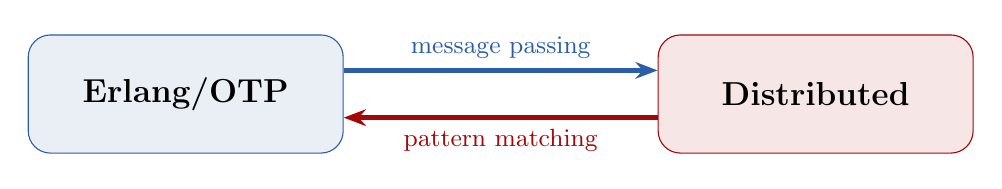
\begin{tikzpicture}
    \node[draw=erlblue, fill=erlblue!10, rounded corners=8pt, minimum width=4cm, minimum height=1.5cm, font=\large\bfseries] (erl) at (0,0) {Erlang/OTP};
    \node[draw=erlred, fill=erlred!10, rounded corners=8pt, minimum width=4cm, minimum height=1.5cm, font=\large\bfseries] (dist) at (8,0) {Distributed};

    \draw[-{Stealth[length=8pt]}, line width=2pt, erlblue]
        ([yshift=3mm]erl.east) -- node[above, font=\small] {message passing} ([yshift=3mm]dist.west);
    \draw[-{Stealth[length=8pt]}, line width=2pt, erlred]
        ([yshift=-3mm]dist.west) -- node[below, font=\small] {pattern matching} ([yshift=-3mm]erl.east);
\end{tikzpicture}

\vspace{3cm}

{\large\color{darkgray} Erlang/OTP Programming Knowledge Collection}

\vspace{1cm}

{\normalsize\color{gray} Concurrent Programming $\cdot$ Distributed Systems $\cdot$ Fault Tolerance}

\vfill
{\small\today}
\end{titlepage}

% ---- Table of Contents ----
\newpage
\tableofcontents
\newpage

% ============================================================
% Section 1: Basics
% ============================================================
\section{基础语法}

\subsection{数据类型转换}

\begin{itemize}[leftmargin=1.5em]
    \item \lstinline|list_to_integer/1| --- 列表转整数
    \item \lstinline|byte_size/1| --- 获取字节大小
\end{itemize}

\subsection{Erlang 的循环}

Erlang 没有传统的循环语句，通过递归和列表操作实现循环逻辑。

\subsubsection{生成一个数组}

\begin{lstlisting}
[X || X <- lists:seq(1,100), X rem 2 == 0].
\end{lstlisting}

\subsubsection{遍历数组}

\begin{lstlisting}
lists:foldl(fun(X, Sum) -> X + Sum end, 0,
    [X || X <- lists:seq(1,100)]).
\end{lstlisting}

\subsubsection{调用 N 次某函数}

\begin{lstlisting}
lists:foldl(fun(X, Sum) ->
    database_logic:storeDB(node(), X) end, 0,
    [X || X <- lists:seq(1,100)]).
\end{lstlisting}

\subsection{模式匹配}

模式匹配（Pattern Matching）在 Erlang 中有三大用途：
\begin{itemize}[leftmargin=1.5em]
    \item 选择控制流分支
    \item 执行变量赋值（绑定）
    \item 分解数据结构（选取和提取部分）
\end{itemize}

\begin{figure}[H]
\centering
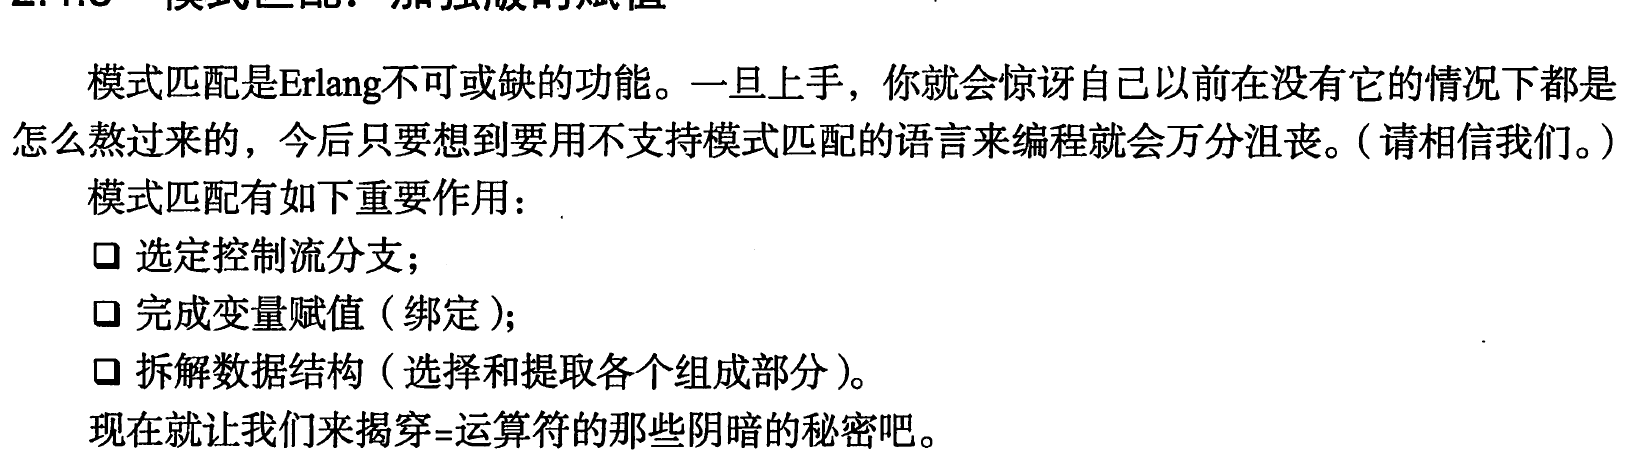
\includegraphics[width=0.85\textwidth]{image56}
\caption{模式匹配}
\end{figure}

\subsubsection{函数参数中的模式匹配}

\begin{figure}[H]
\centering
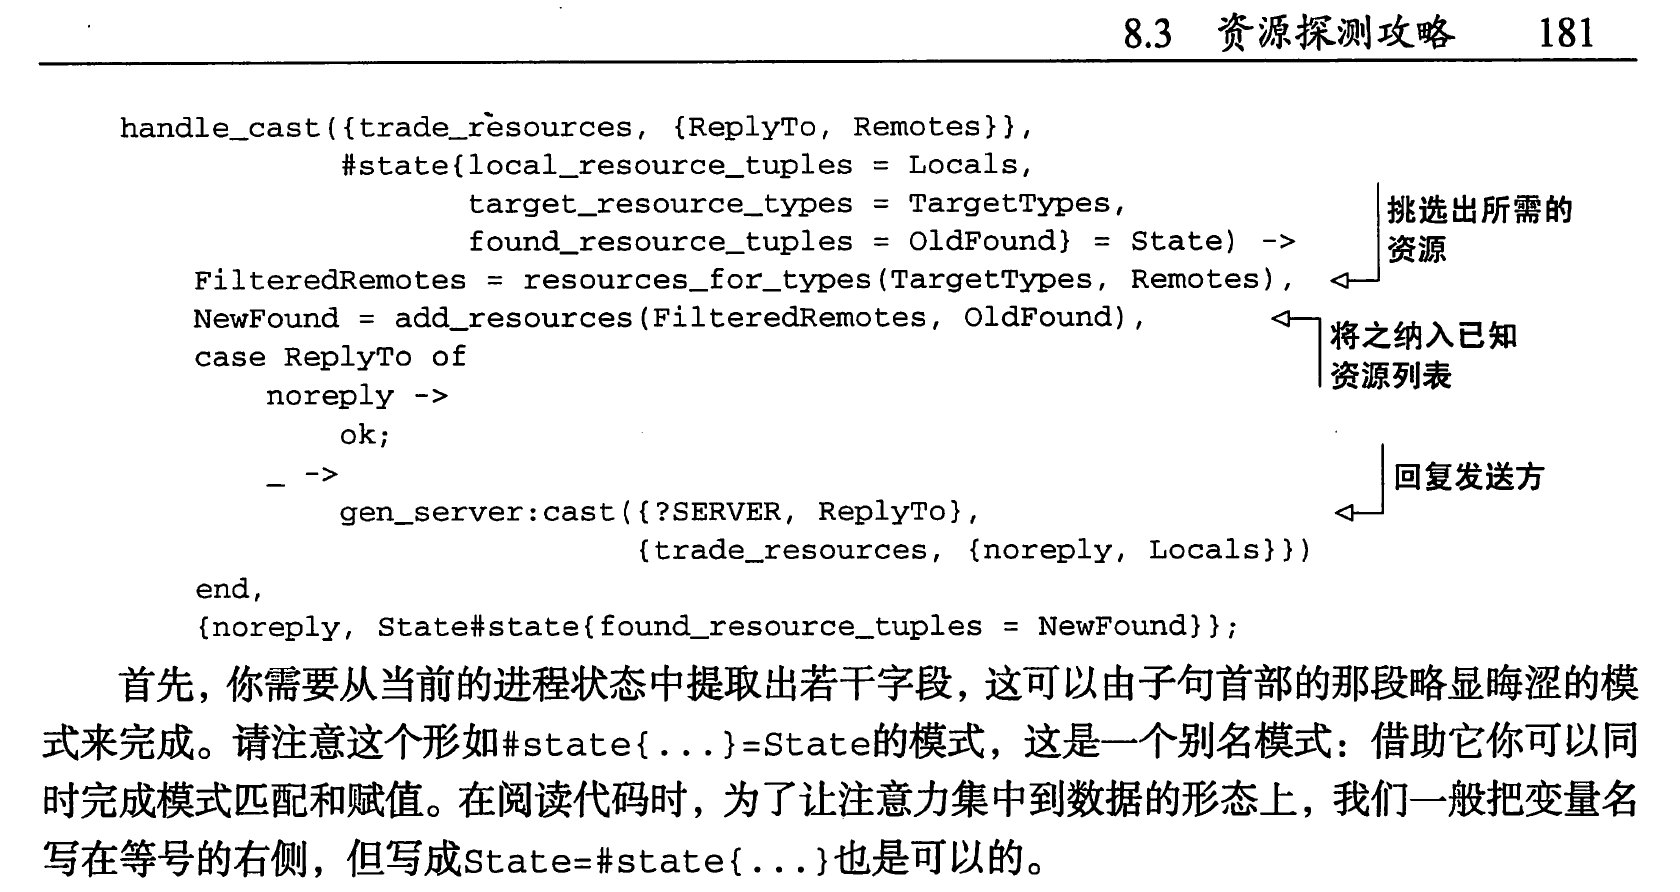
\includegraphics[width=0.85\textwidth]{image57}
\caption{函数参数中的模式匹配}
\end{figure}

\begin{notebox}[Alias Pattern]
The pattern has the shape \lstinline|#state{...}=State|, which means it's an alias pattern: it both matches and assigns a name at the same time.
\end{notebox}

\subsection{短路求值}

\begin{lstlisting}
Expr1 orelse Expr2
Expr1 andalso Expr2
\end{lstlisting}

详见：\href{https://www.erlang.org/doc/reference_manual/expressions.html}{Erlang -- Expressions}

\subsection{begin...end}

\lstinline|begin...end| 用于将多个表达式组合为一个表达式，常见于 \lstinline|if|、\lstinline|case| 等需要单表达式的地方。

\begin{figure}[H]
\centering
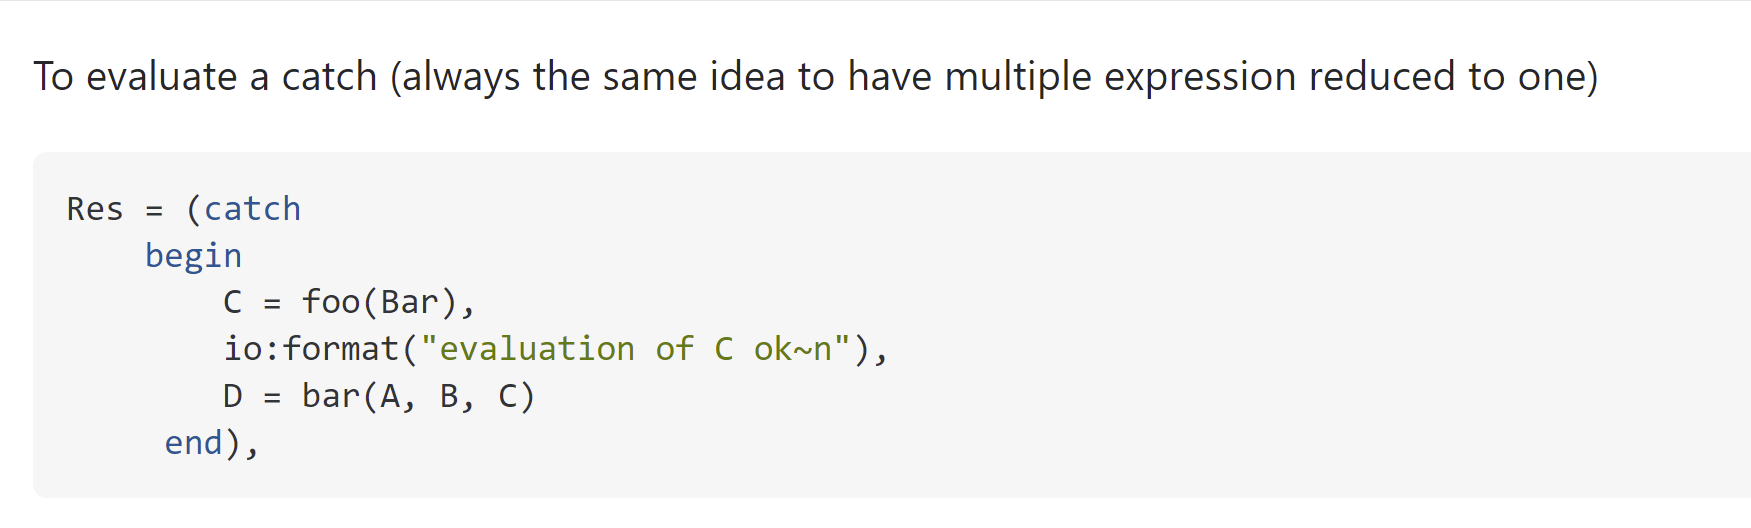
\includegraphics[width=0.85\textwidth]{image41}
\caption{begin...end 用法}
\end{figure}

\begin{figure}[H]
\centering
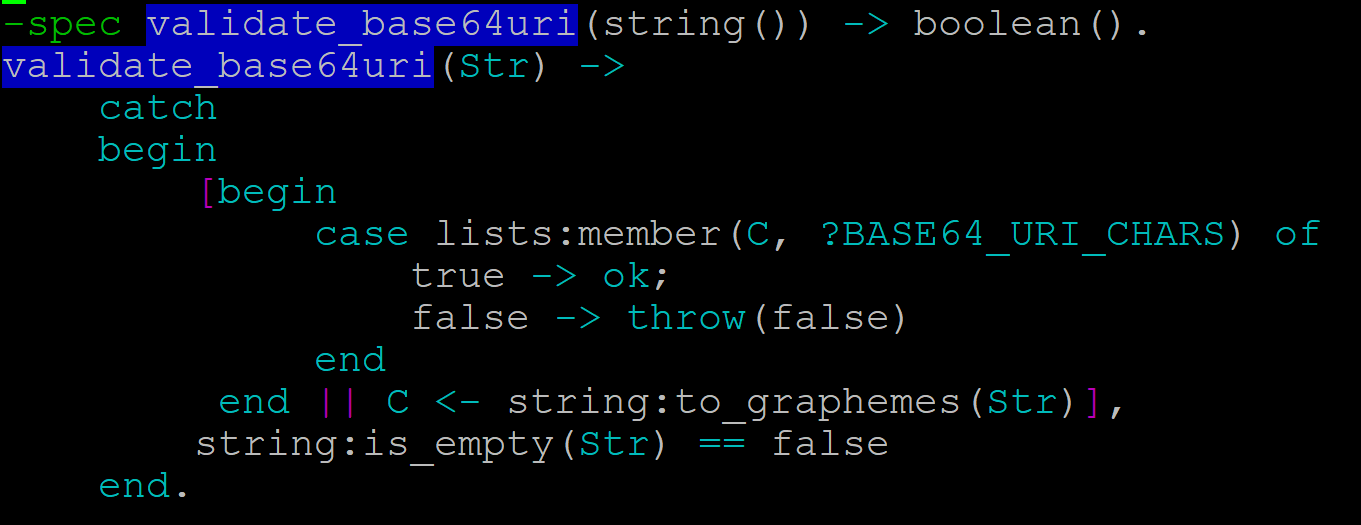
\includegraphics[width=0.85\textwidth]{image42}
\caption{begin...end 示例}
\end{figure}

\begin{figure}[H]
\centering
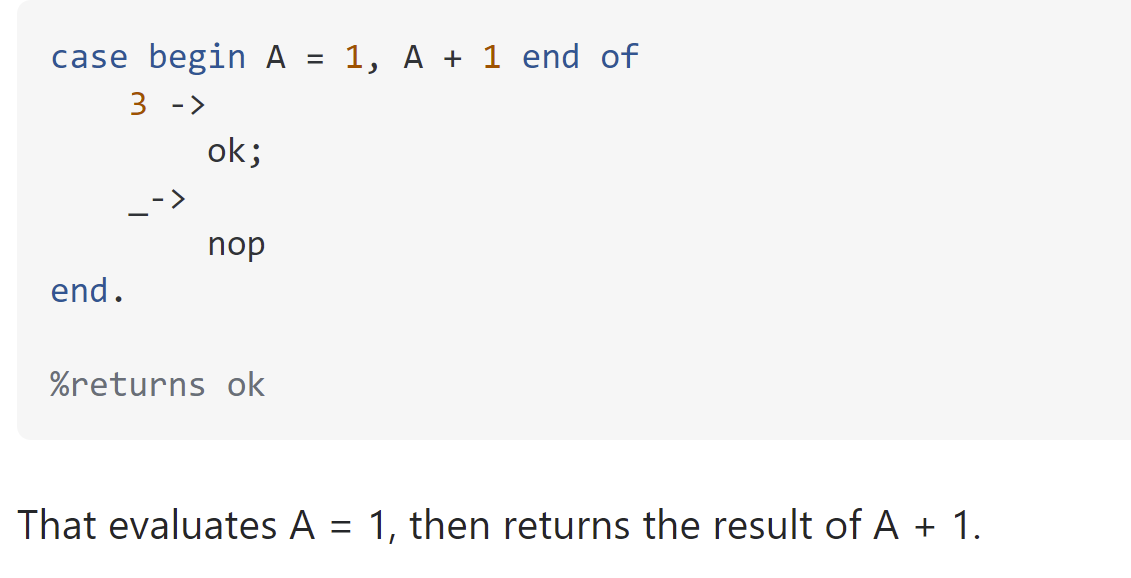
\includegraphics[width=0.7\textwidth]{image43}
\caption{begin...end 代码块}
\end{figure}

\begin{figure}[H]
\centering
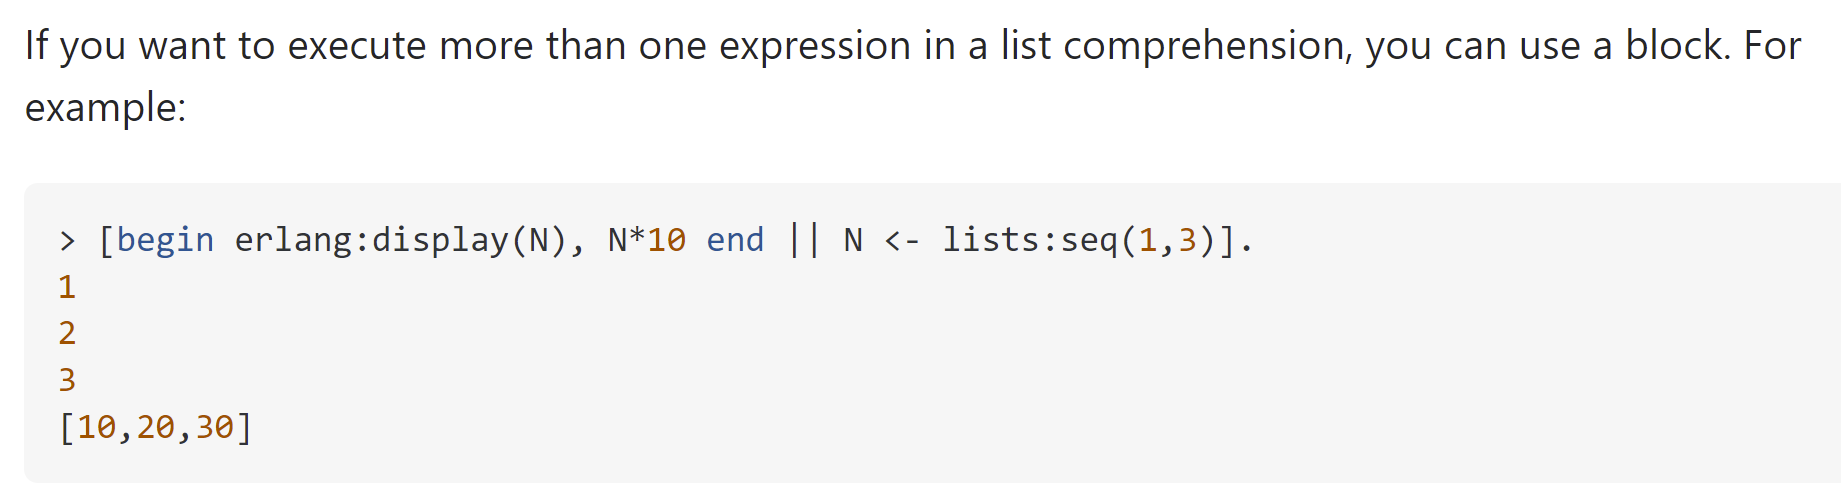
\includegraphics[width=0.85\textwidth]{image44}
\caption{begin...end 执行结果}
\end{figure}

\subsection{list comprehension}

列表推导式（List Comprehension）是 Erlang 中强大的语法特性。

\begin{itemize}[leftmargin=1.5em]
    \item 结合 \lstinline|lists:delete/2| 使用
    \item 调试时临时函数名的解读：参见 \href{https://stackoverflow.com/questions/6019447/how-to-read-decode-temporary-function-names-of-list-comprehension-in-erlang-when}{Stack Overflow}
\end{itemize}

\subsection{\$ Dollar Sign}

\begin{figure}[H]
\centering
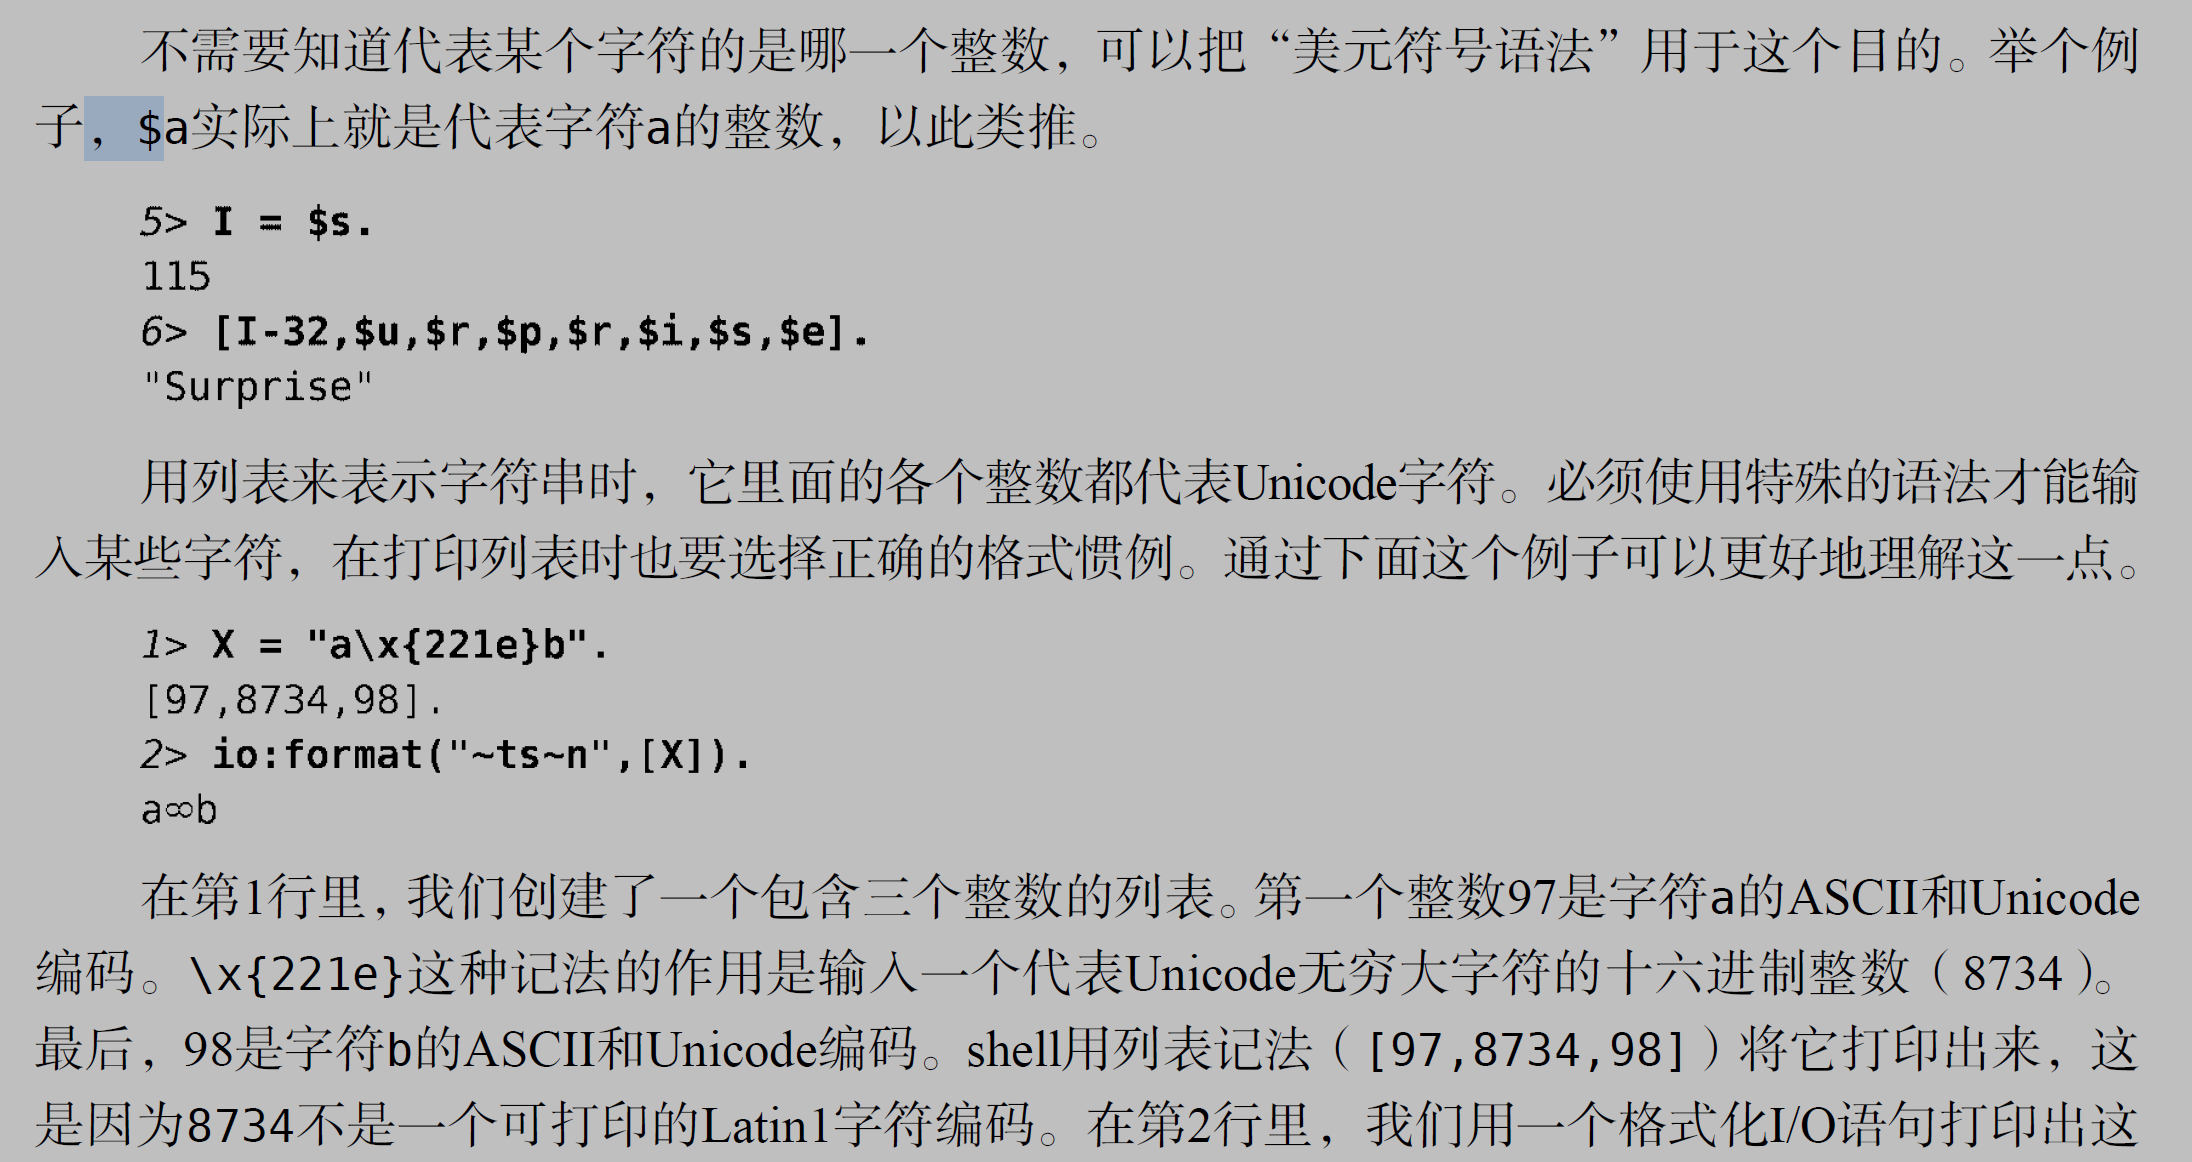
\includegraphics[width=0.85\textwidth]{image45}
\caption{\$ 符号用法}
\end{figure}

\subsection{lists:takewhile}

\begin{figure}[H]
\centering
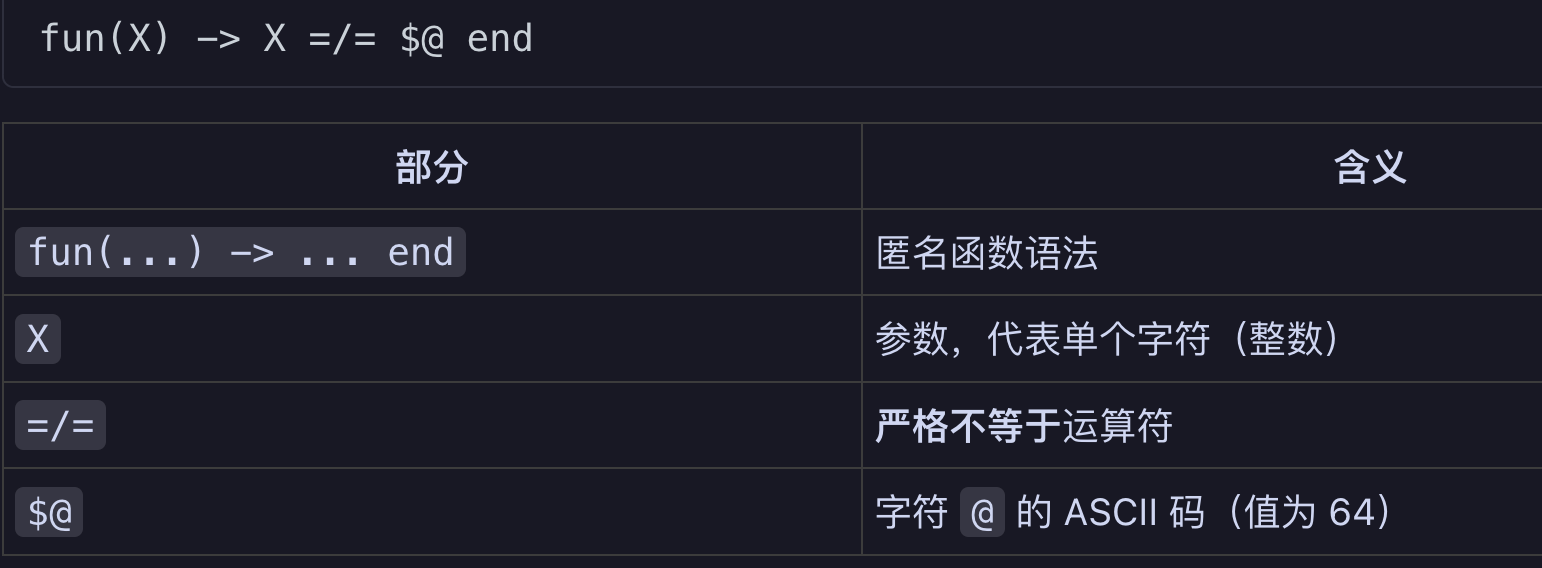
\includegraphics[width=0.8\textwidth]{image46}
\caption{lists:takewhile 示例}
\end{figure}

\subsection{Erlang 没有 continue 关键字}

It's not a keyword, it is simply an atom returned as result of the fun.

\subsection{Closures in Erlang}

Erlang 支持闭包（Closures），函数可以捕获其定义环境中的变量。

参考：\href{https://navidmostafiz.medium.com/closures-in-erlang-made-easy-708936749608}{Closures in Erlang Made Easy}

% ============================================================
% Section 2: Module Attributes
% ============================================================
\section{模块属性（Module Attributes）}

\subsection{基本属性}

\begin{figure}[H]
\centering
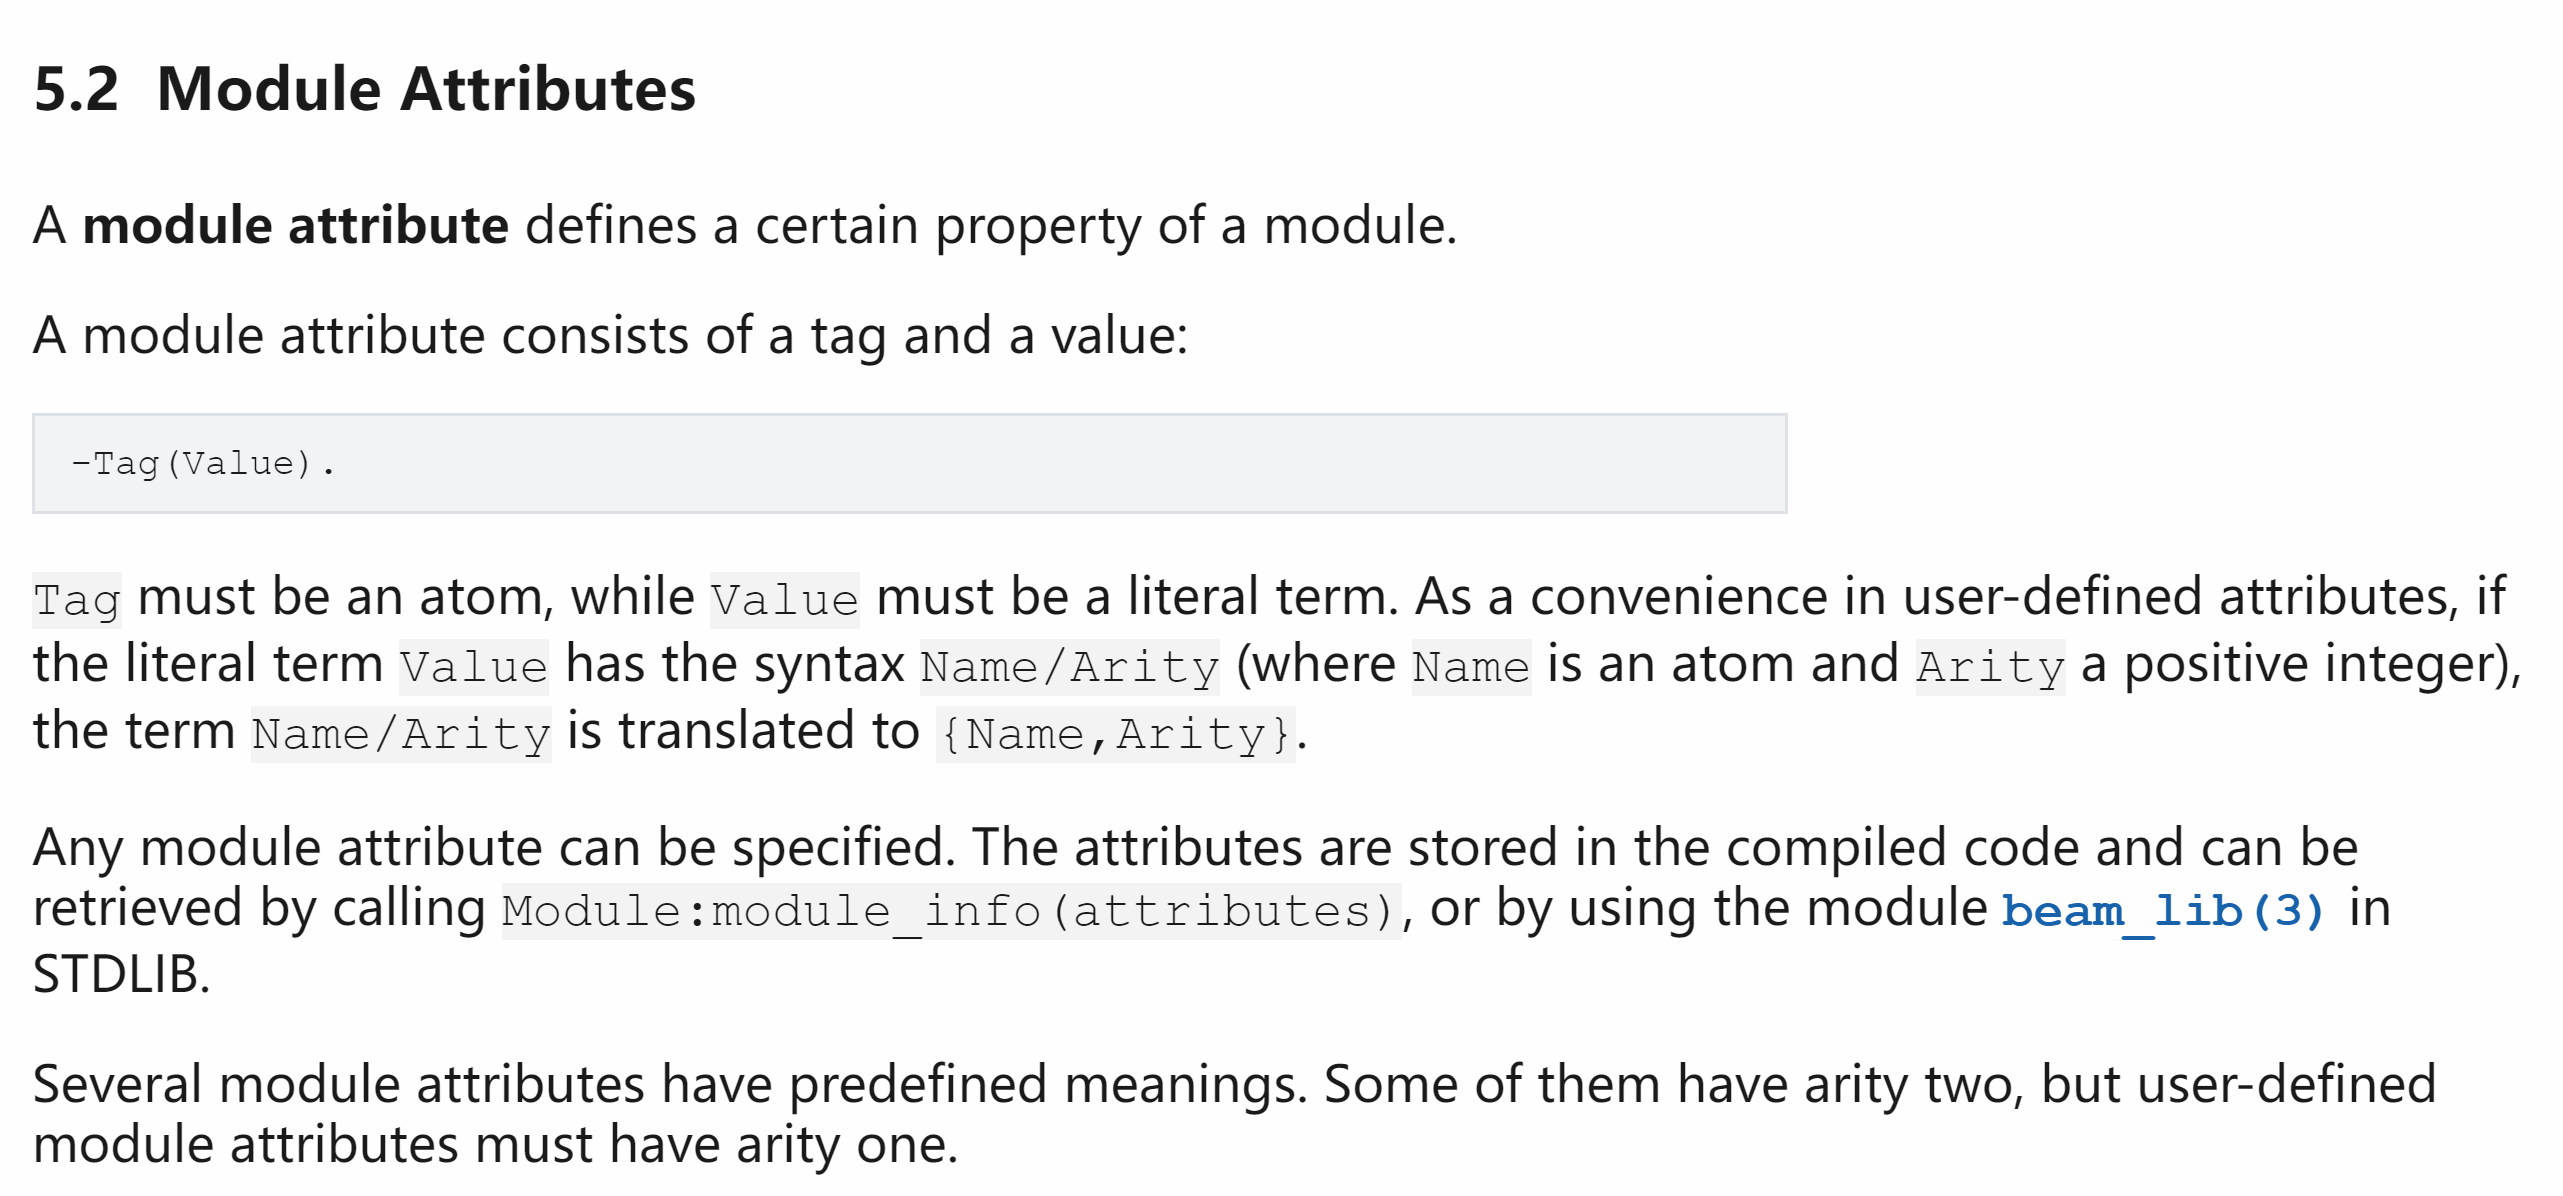
\includegraphics[width=0.85\textwidth]{image3}
\caption{Module Attributes 概览}
\end{figure}

\begin{figure}[H]
\centering
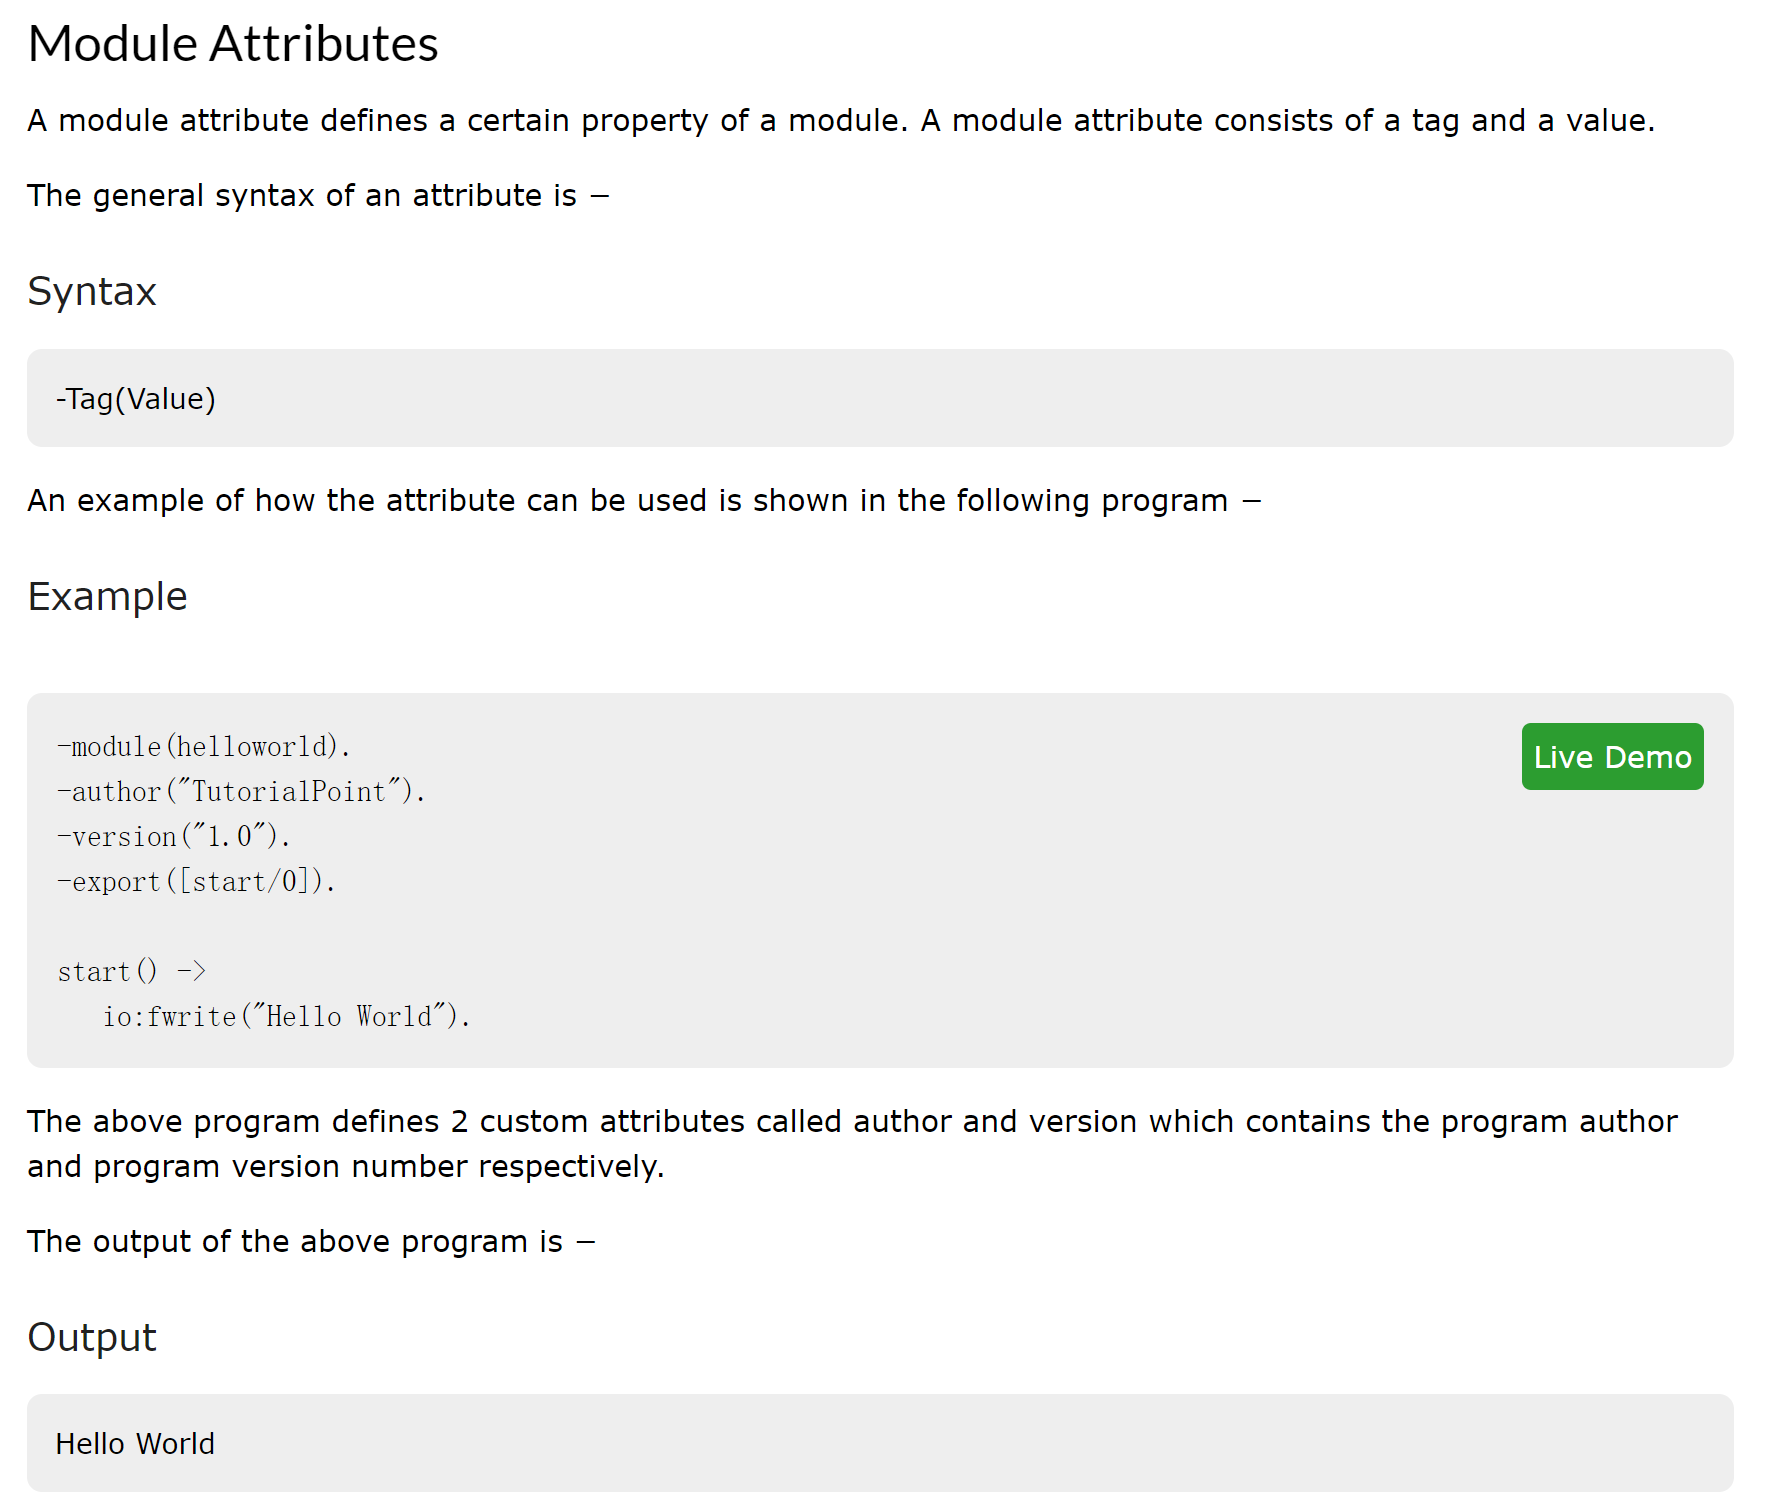
\includegraphics[width=0.85\textwidth]{image4}
\caption{Module Attributes 详解}
\end{figure}

参考：
\begin{itemize}[leftmargin=1.5em]
    \item \href{https://www.erlang.org/doc/reference_manual/modules}{Erlang -- Modules}
    \item \href{https://www.tutorialspoint.com/erlang/erlang_modules.htm}{Erlang - Modules (TutorialsPoint)}
\end{itemize}

\subsection{Tuple 形式的模块属性}

Tuple 形式的属性与普通属性没有任何差别，例如：

\begin{lstlisting}
-module(rabbit).
-author("TutorialPoint").
-version("1.0").
-module_description("This is an example module.").

-rabbit_boot_step({pre_boot,
    [{description, "rabbit boot start"}]}).

-rabbit_boot_step({codec_correctness_check,
    [{description, "codec correctness check"},
     {mfa, {rabbit_binary_generator,
            check_empty_frame_size, []}},
     {requires, pre_boot},
     {enables, external_infrastructure}]}).

-export([start/0]).
-export([start1/0]).

start() ->
    io:fwrite("Hello World\n"),
    ModuleInfo = rabbit:module_info(),
    Attributes = rabbit:module_info(attributes),
    io:format("~p~n", [Attributes]),
    finish.
\end{lstlisting}

\begin{notebox}[要点]
Any module attribute can be specified. The attributes are stored in the compiled code and can be retrieved by calling \lstinline|Module:module_info(attributes)|, or by using the module \lstinline|beam_lib(3)| in STDLIB.
Tuple 形式的属性值是叠加的。
\end{notebox}

% ============================================================
% Section 3: Distributed Programming
% ============================================================
\section{分布式编程}

\subsection{从配置中启动 MQ}

\begin{enumerate}[leftmargin=1.5em]
    \item \lstinline|.erlang.cookie| 文件必须一致
    \item 必须一次性成功，把节点全部启动起来
\end{enumerate}

\subsection{Hidden Node}

\begin{figure}[H]
\centering
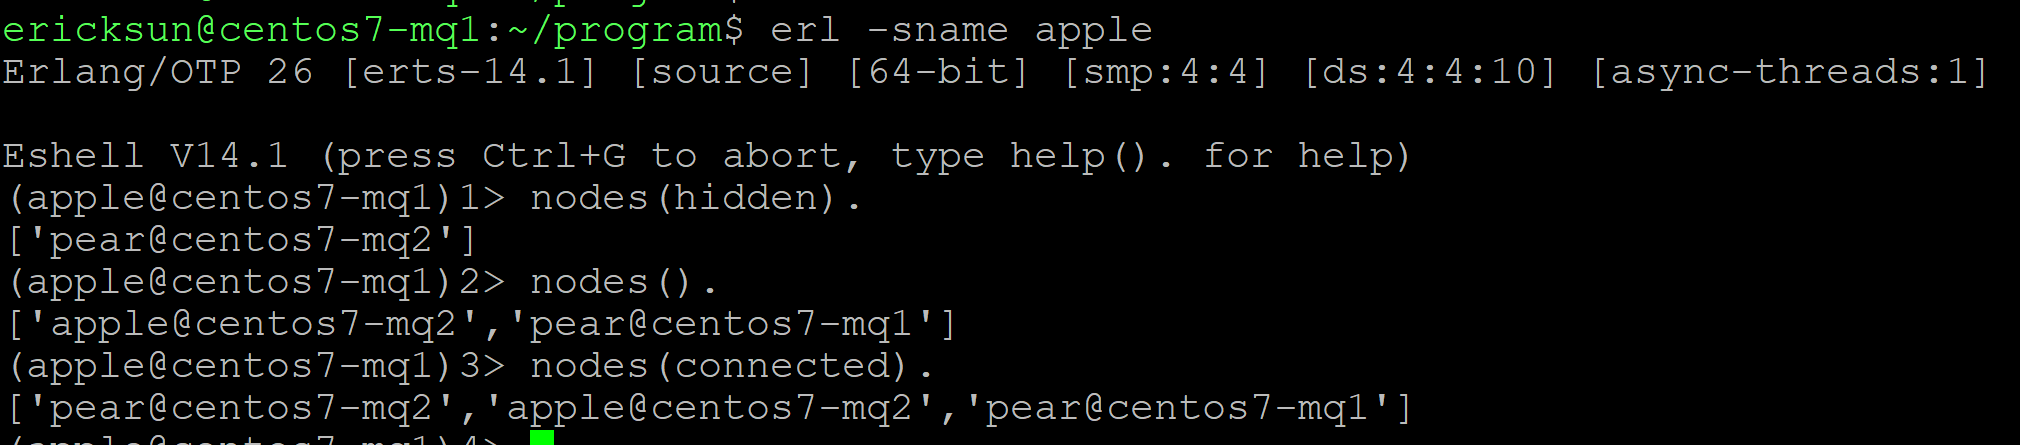
\includegraphics[width=0.85\textwidth]{image1}
\caption{Hidden Node}
\end{figure}

参考：\href{https://www.erlang.org/doc/reference_manual/distributed.html}{Erlang -- Distributed Erlang}

\subsection{远程连接 Erlang 节点}

\subsubsection{使用 remsh}

远程连接的最简方式。

\subsubsection{使用 net\_kernel:connect\_node}

\begin{lstlisting}[style=shellstyle]
[root@kvm_10_21_1_163 sbin]# erl -sname apple
(apple@kvm_10_21_1_163)1> net_kernel:connect_node('rabbit@kvm_10_20_1_60').
true
\end{lstlisting}

\begin{warnbox}[注意]
\lstinline|net_kernel:connect_node/1| 的返回值可能被忽略，参见 \href{https://blog.differentpla.net/blog/2013/11/07/net-kernel-connect-node-1-returns-ignored/}{net\_kernel:connect\_node/1 returns ignored}
\end{warnbox}

需要给节点起个名字（\lstinline|-sname|）才能连接。

\subsubsection{使用 net\_adm:ping}

注意是 \lstinline|-sname| 生效，不用 \lstinline|-name|，能够在远程节点生效。

\begin{figure}[H]
\centering
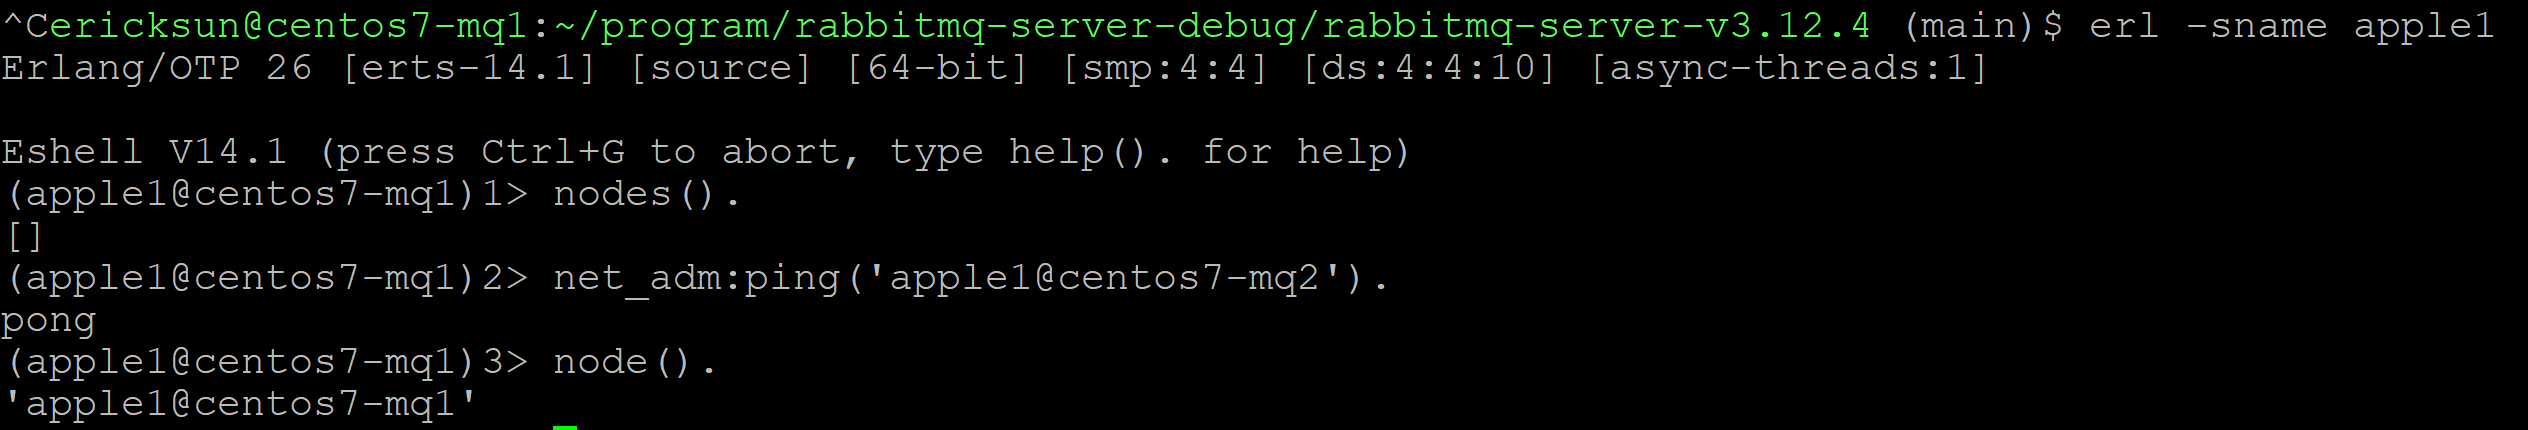
\includegraphics[width=0.85\textwidth]{image5}
\caption{net\_adm:ping 远程连接}
\end{figure}

\subsubsection{使用 rpc:call}

\begin{figure}[H]
\centering
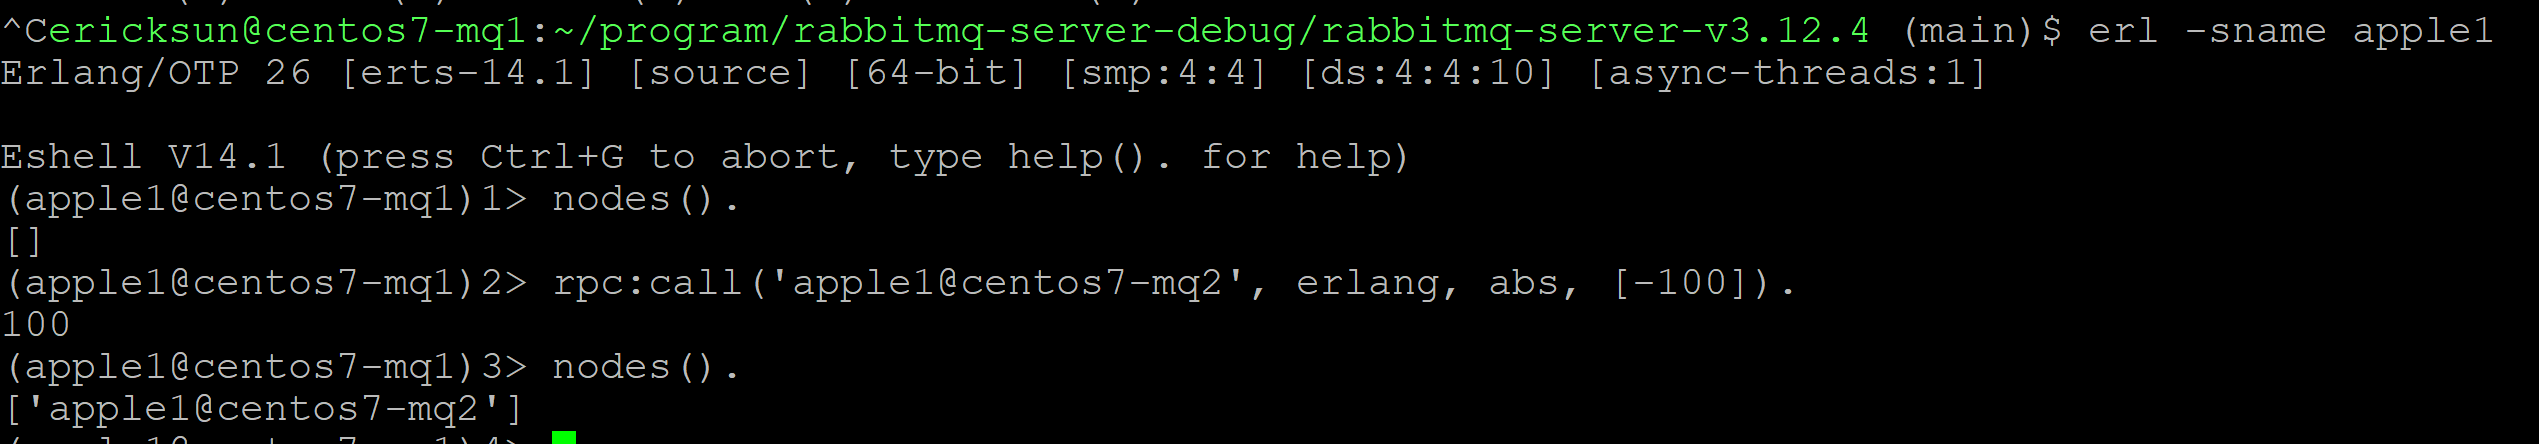
\includegraphics[width=0.85\textwidth]{image6}
\caption{rpc:call 远程调用}
\end{figure}

\subsubsection{使用消息发送 !}

\begin{figure}[H]
\centering
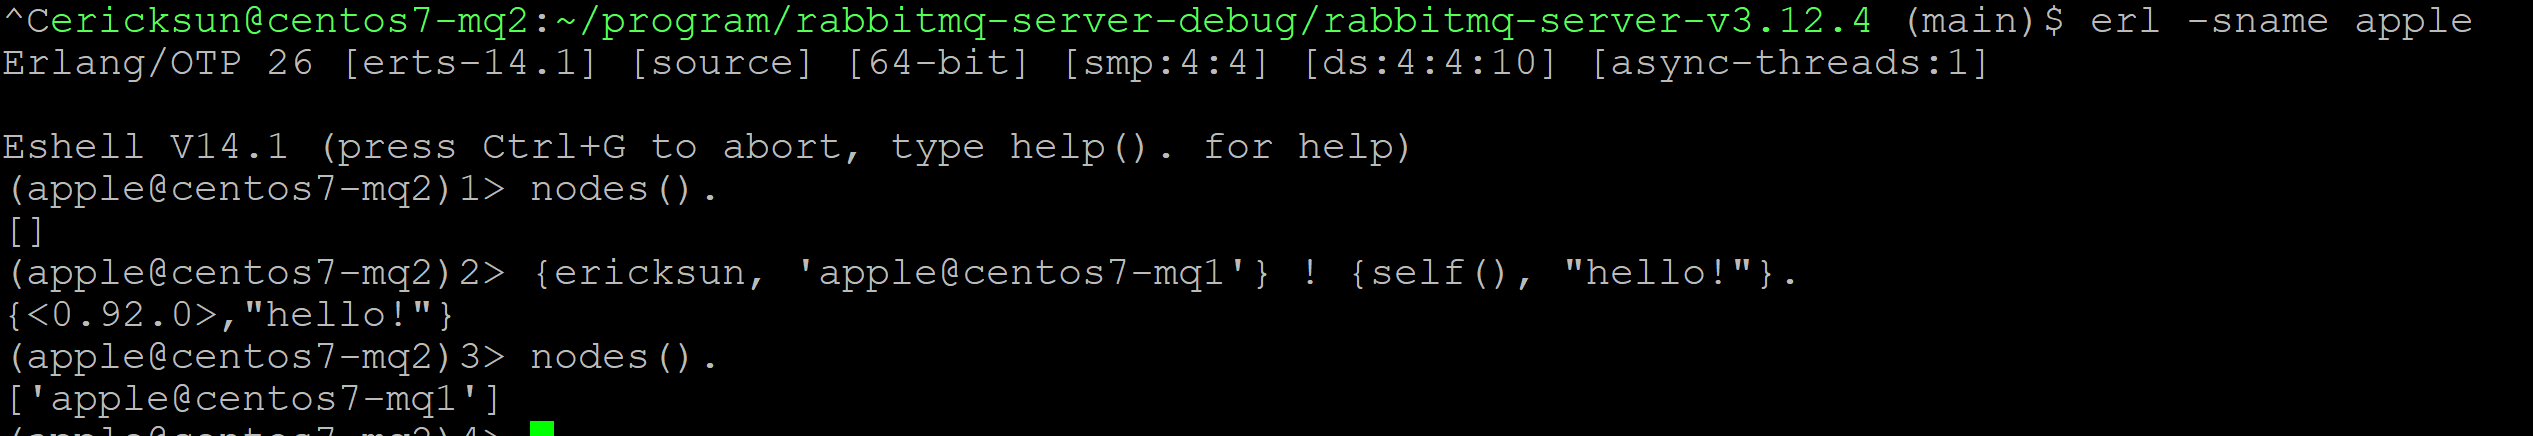
\includegraphics[width=0.85\textwidth]{image7}
\caption{消息发送 ! 远程通信}
\end{figure}

\begin{figure}[H]
\centering
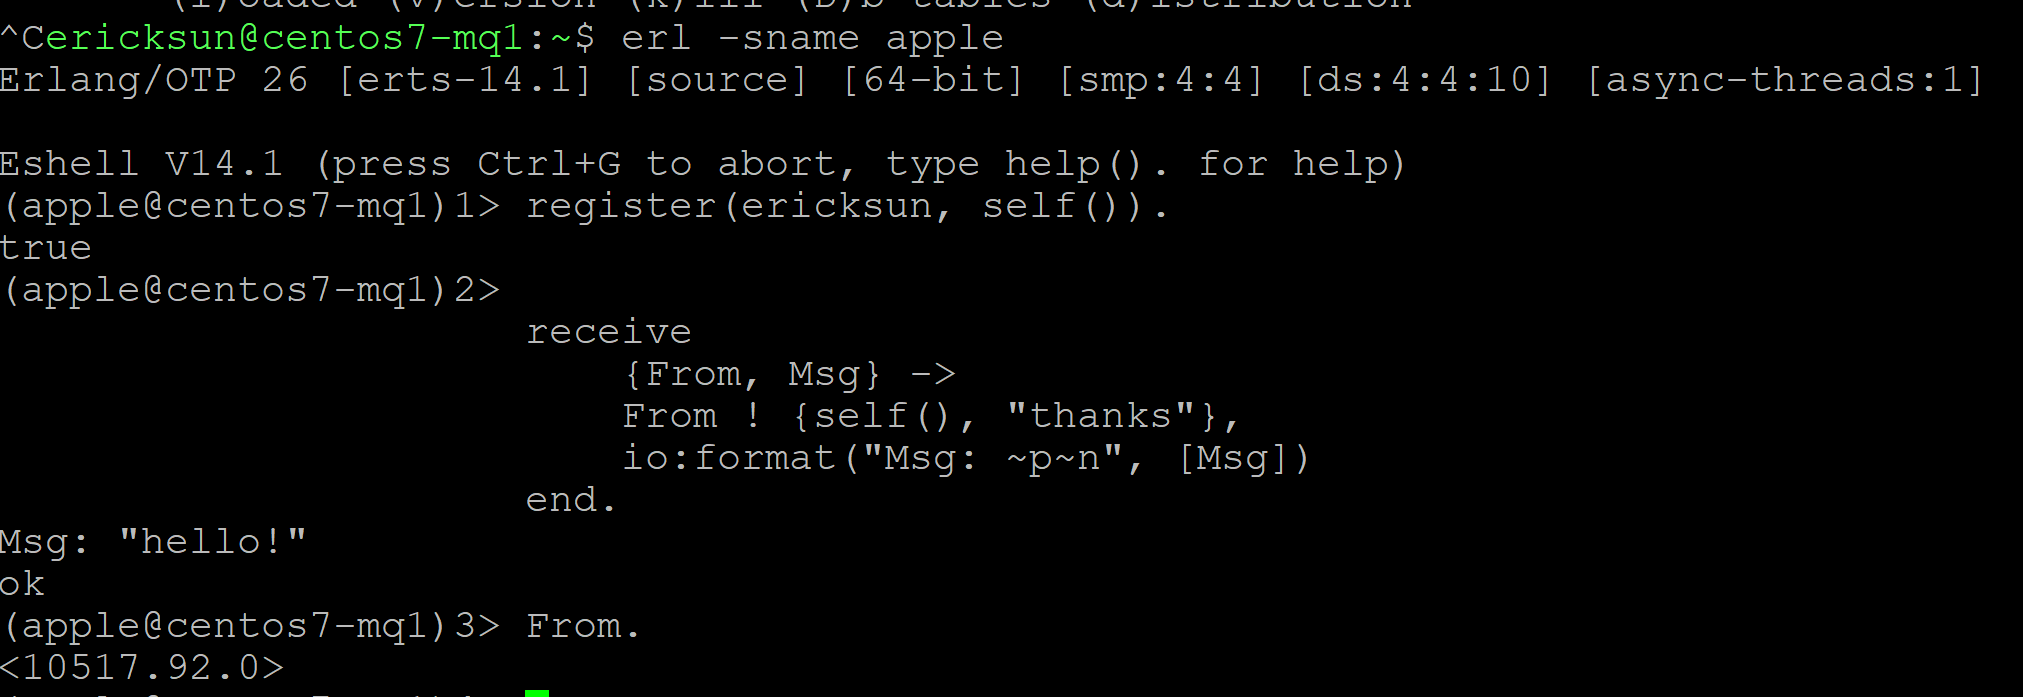
\includegraphics[width=0.85\textwidth]{image8}
\caption{消息发送示例}
\end{figure}

\subsubsection{使用 monitor}

\begin{figure}[H]
\centering
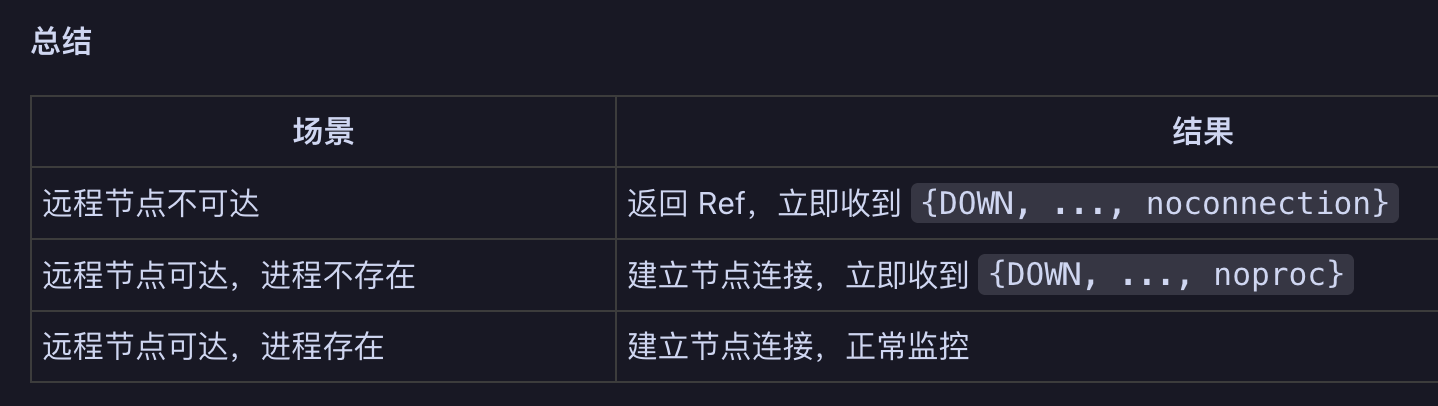
\includegraphics[width=0.8\textwidth]{image9}
\caption{monitor 用法 (1)}
\end{figure}

\begin{figure}[H]
\centering
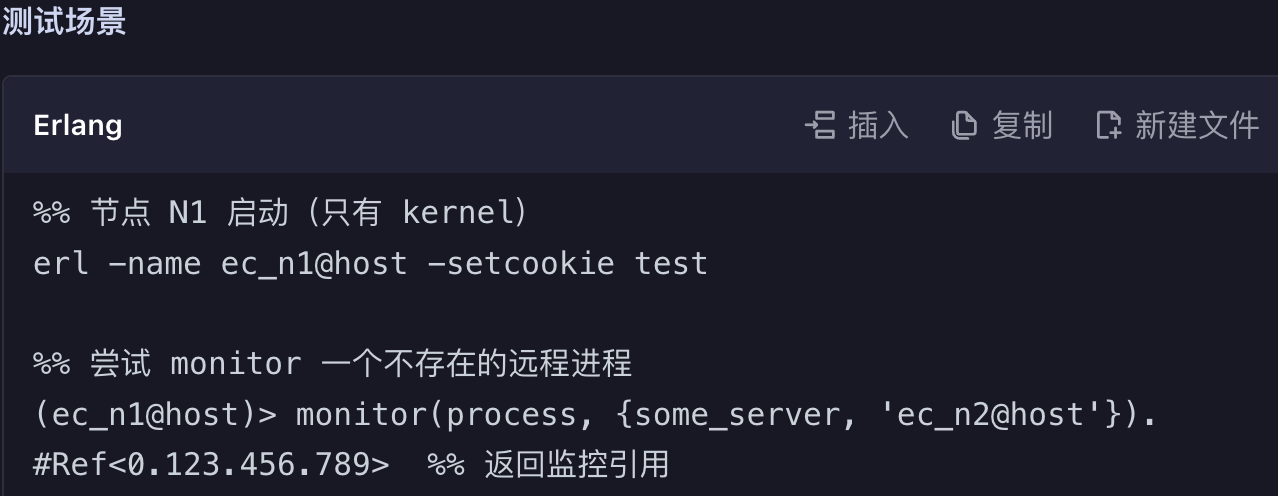
\includegraphics[width=0.6\textwidth]{image10}
\caption{monitor 用法 (2)}
\end{figure}

\begin{figure}[H]
\centering
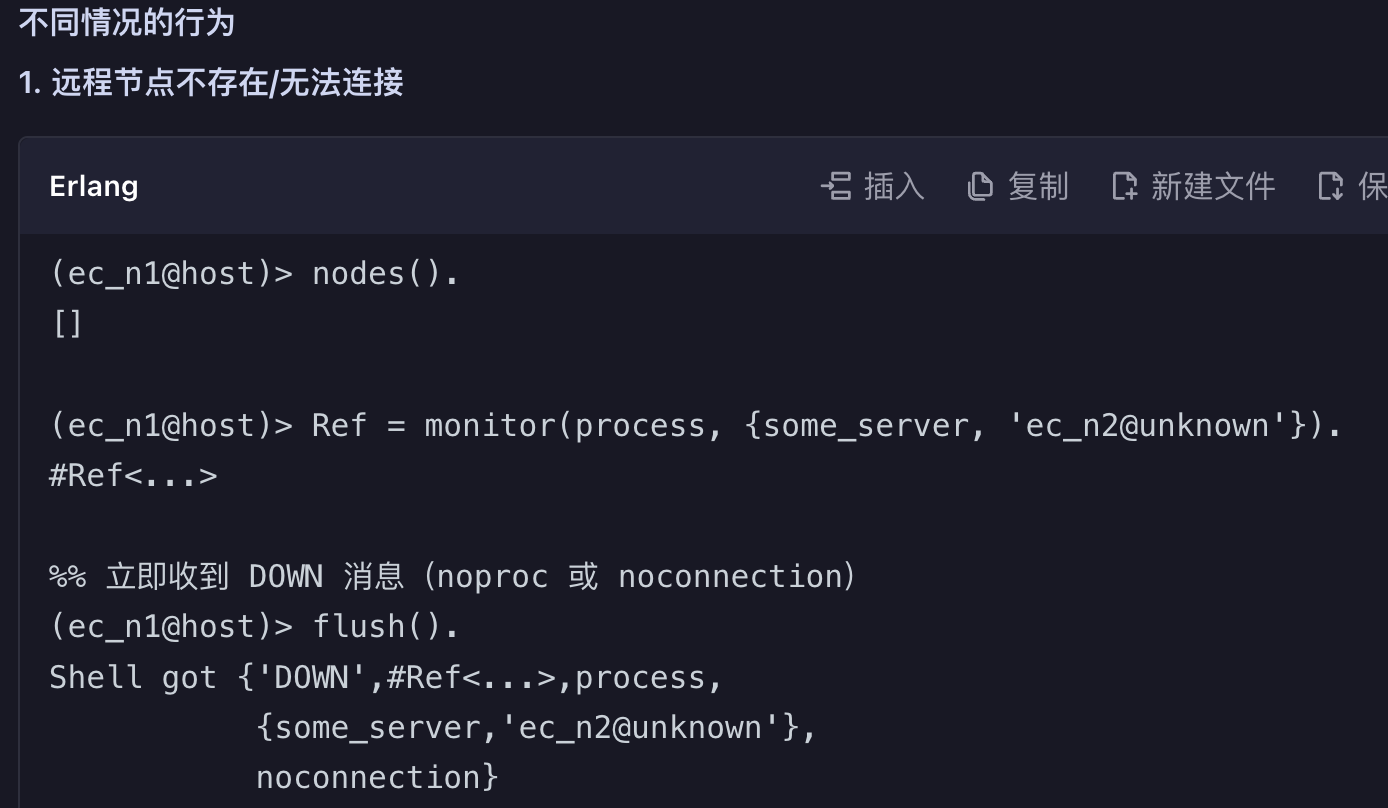
\includegraphics[width=0.7\textwidth]{image11}
\caption{monitor 用法 (3)}
\end{figure}

\begin{figure}[H]
\centering
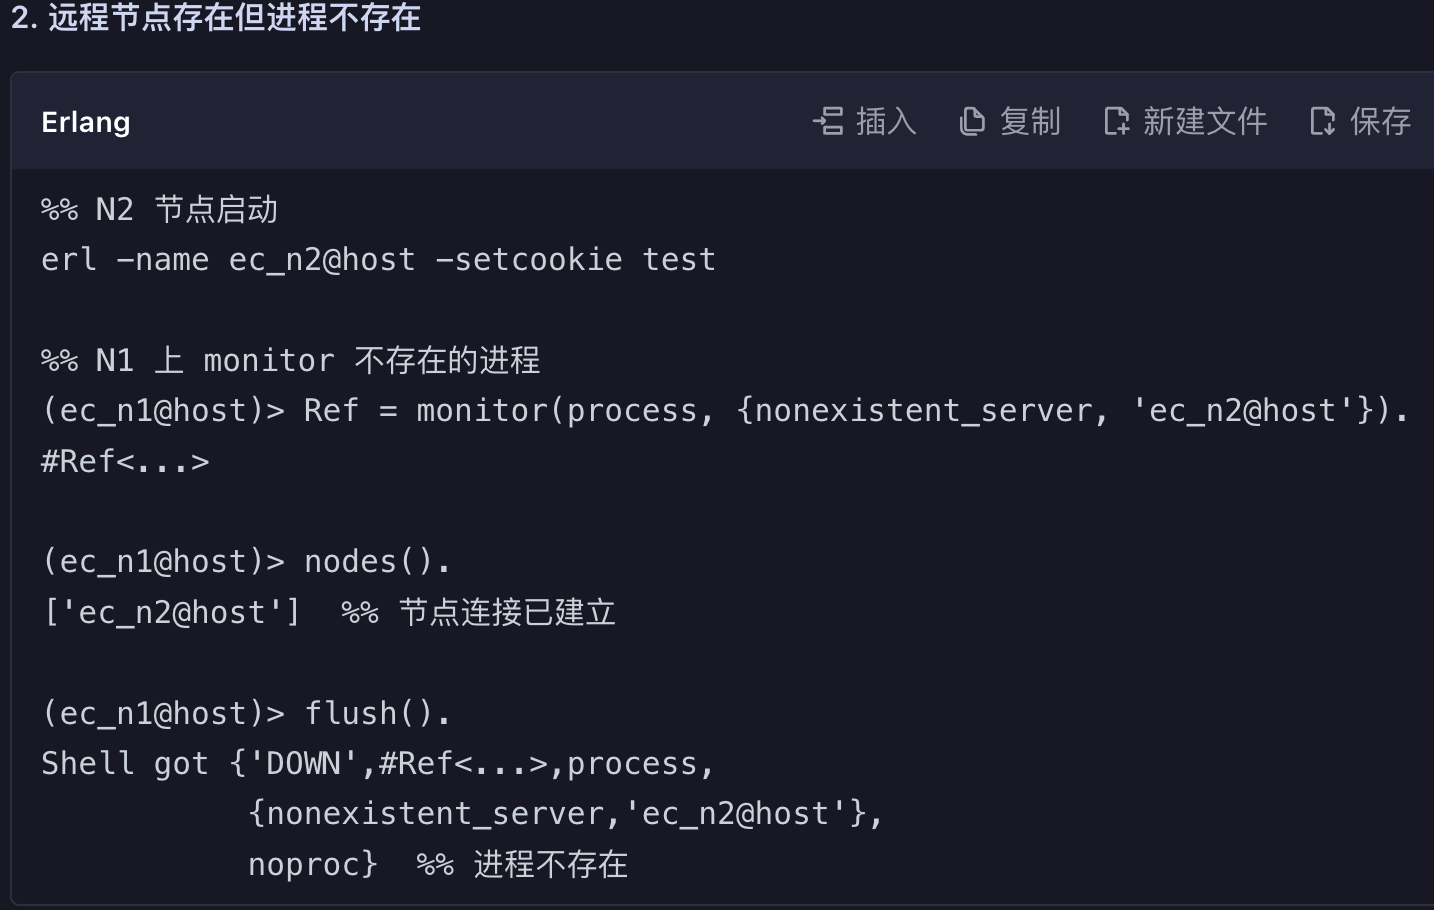
\includegraphics[width=0.65\textwidth]{image12}
\caption{monitor 用法 (4)}
\end{figure}

\begin{figure}[H]
\centering
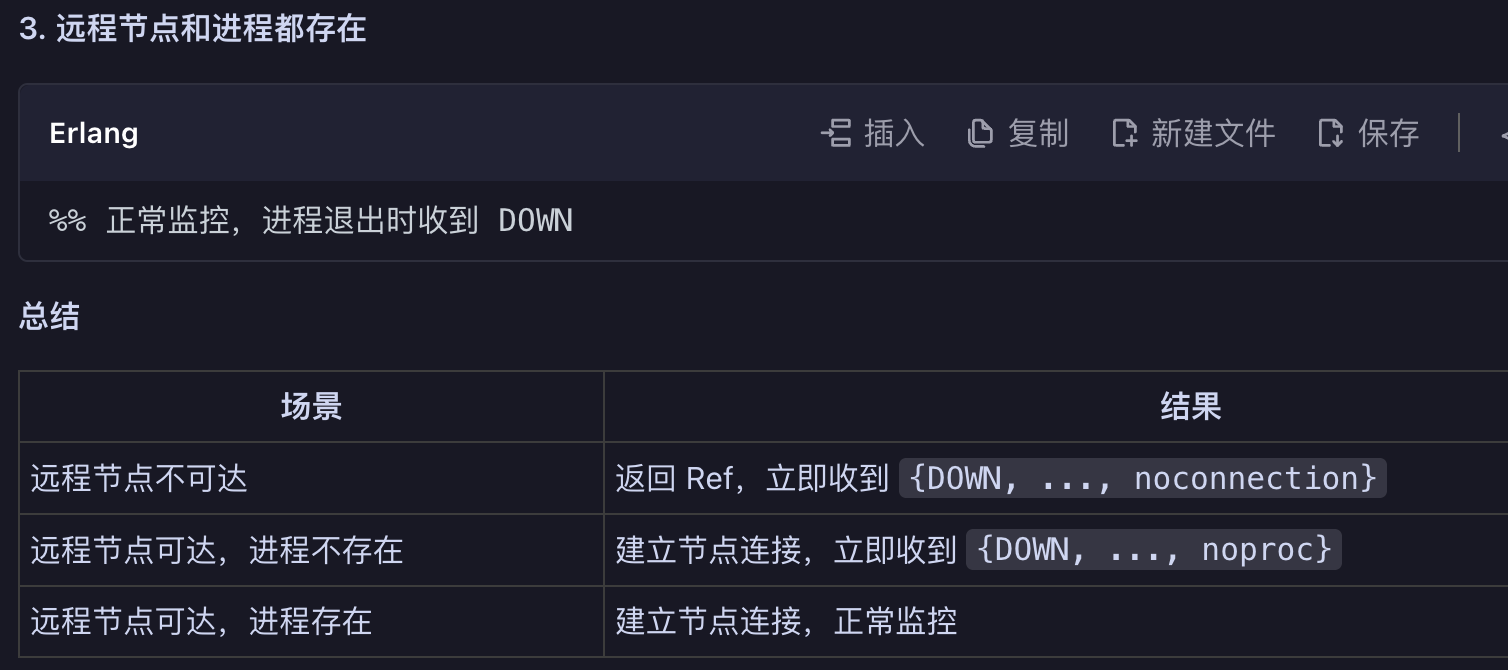
\includegraphics[width=0.65\textwidth]{image13}
\caption{monitor 用法 (5)}
\end{figure}

三种情况：
\begin{enumerate}[leftmargin=1.5em]
    \item Case 1: 节点不存在
    \item Case 2: 节点存在，服务不存在，建立连接
    \item Case 3: 远程节点和进程都存在
\end{enumerate}

\subsubsection{使用 Ctrl+G}

通过 Ctrl+G 可以连接到远程节点。

\subsubsection{使用 Observer 观察远程节点}

注意在本地先启动 observer，然后在 Nodes 中切换。

\textbf{步骤：}

\begin{enumerate}[leftmargin=1.5em]
    \item 新起一个节点
\end{enumerate}

\begin{figure}[H]
\centering
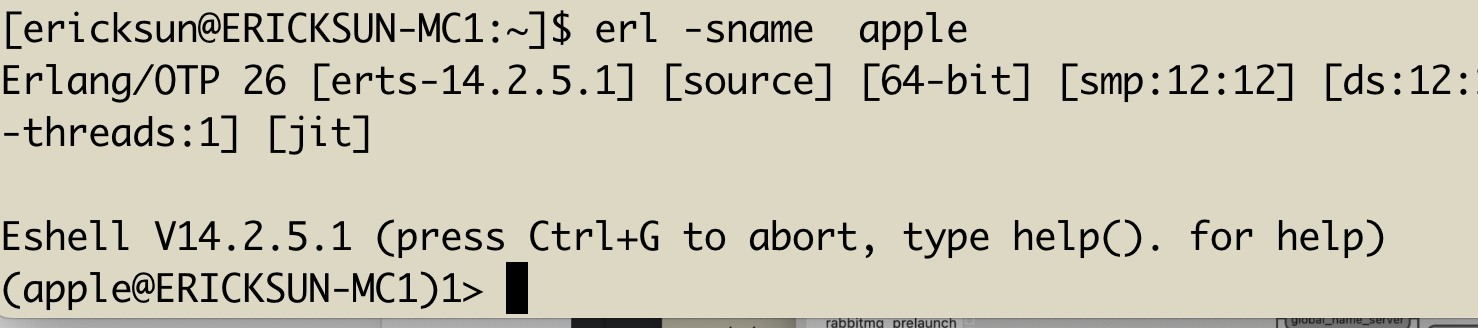
\includegraphics[width=0.85\textwidth]{image14}
\caption{新起节点}
\end{figure}

\begin{enumerate}[leftmargin=1.5em]
    \setcounter{enumi}{1}
    \item 启动 observer
\end{enumerate}

\begin{figure}[H]
\centering
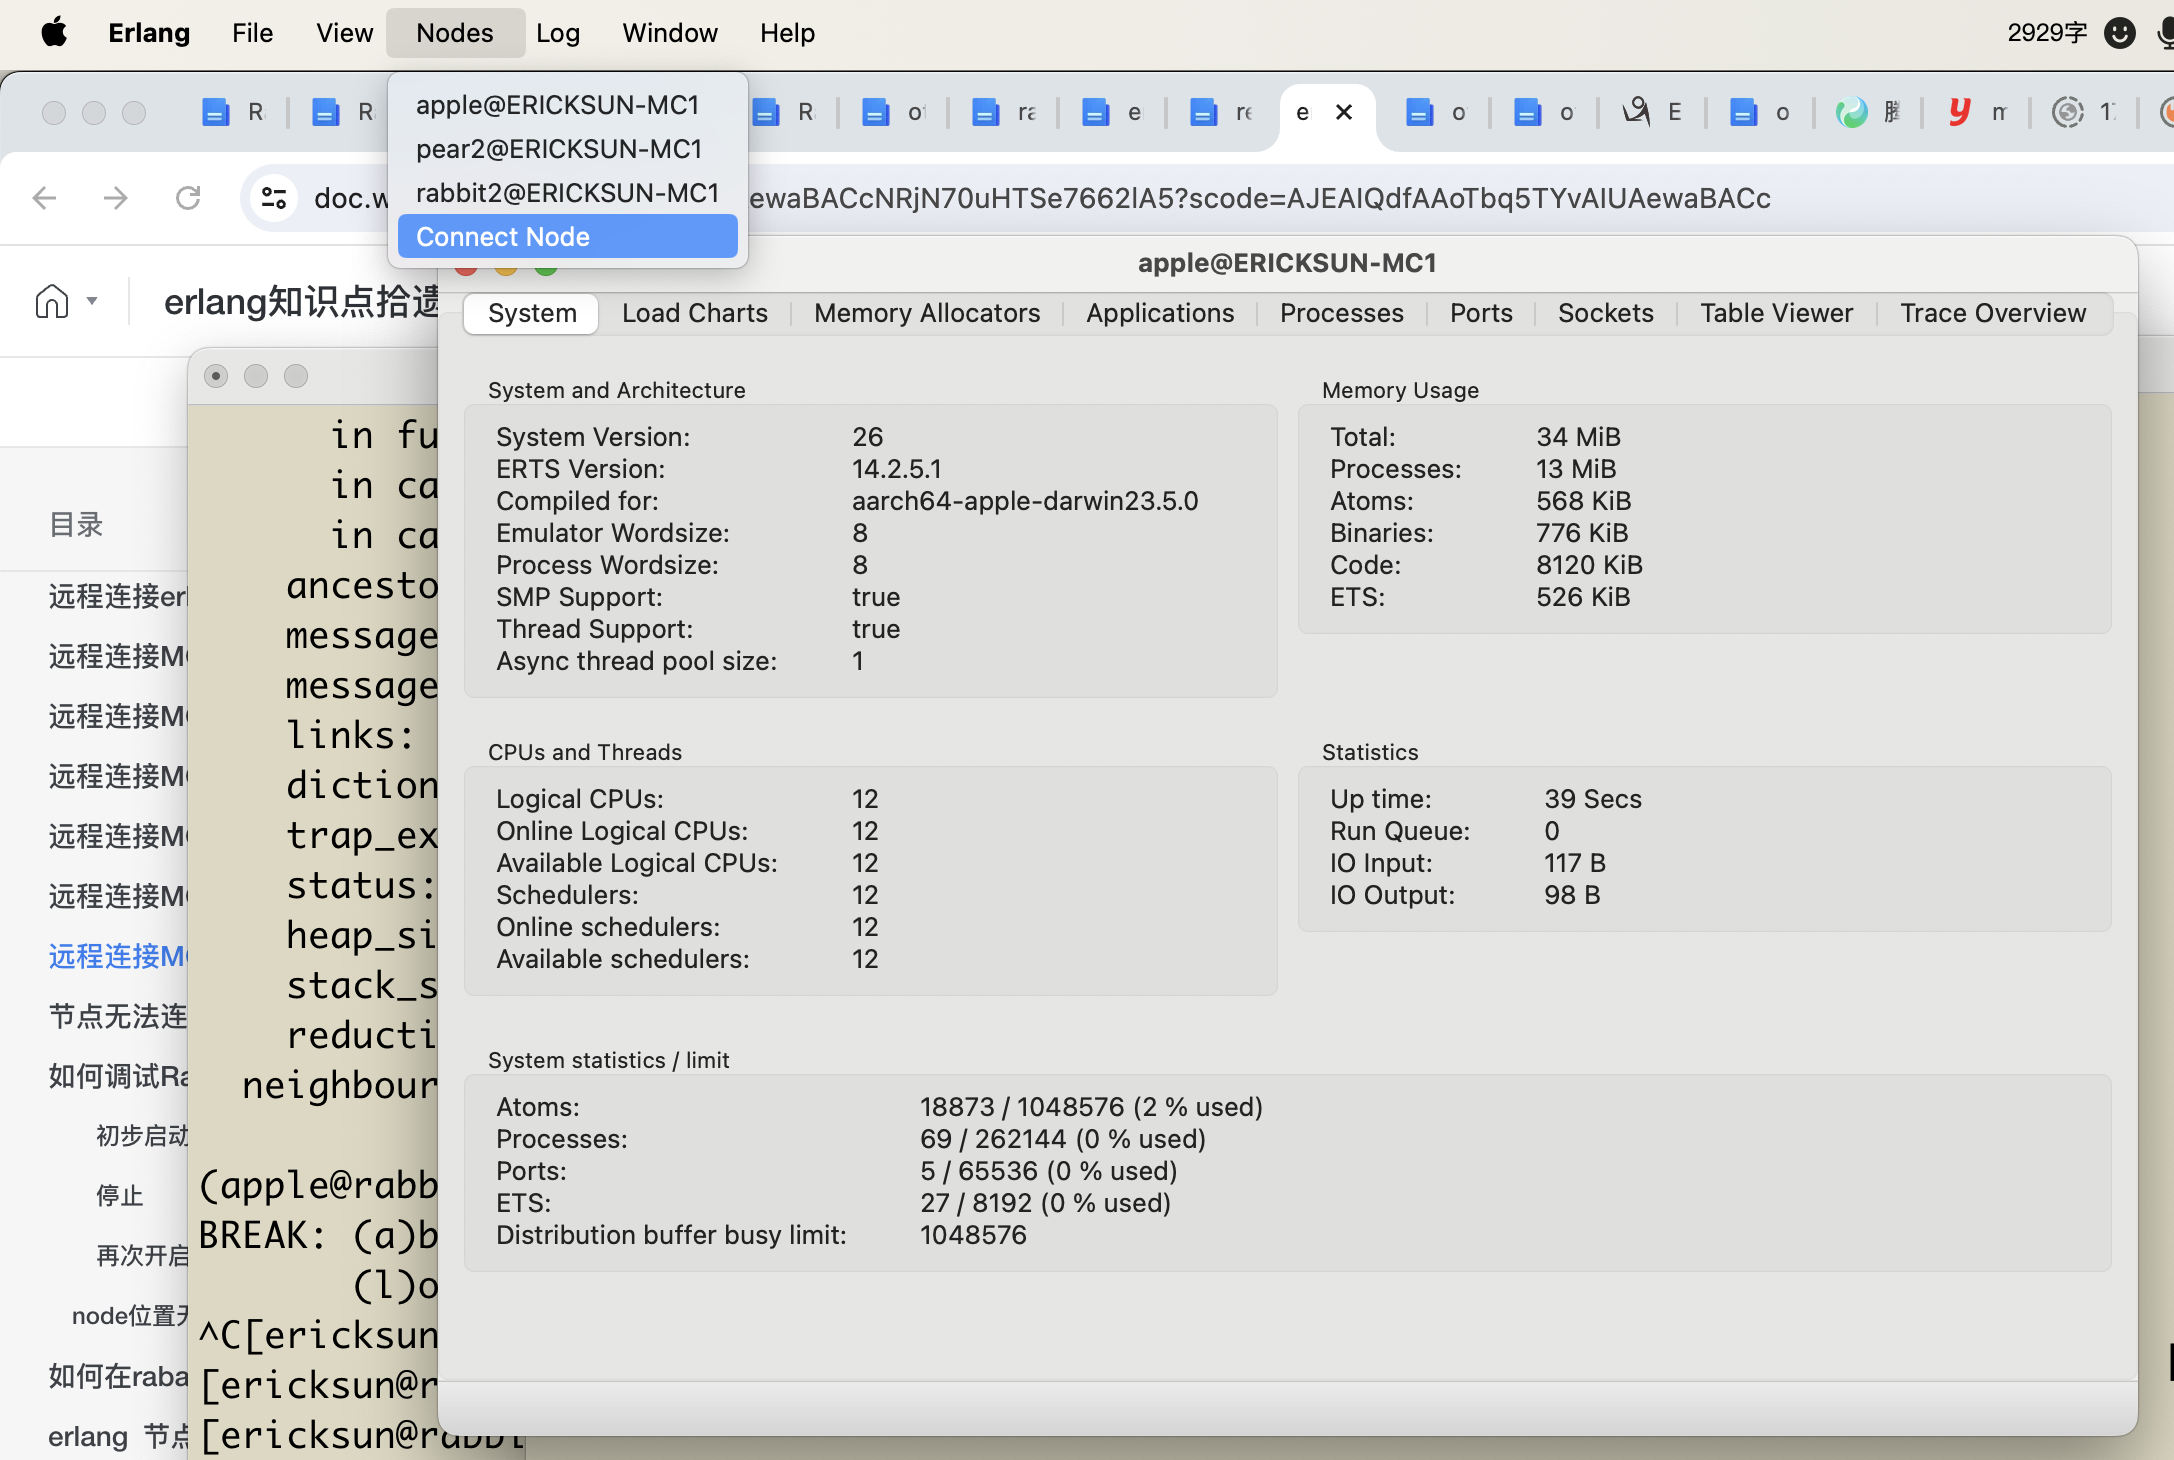
\includegraphics[width=0.85\textwidth]{image15}
\caption{启动 observer}
\end{figure}

\begin{enumerate}[leftmargin=1.5em]
    \setcounter{enumi}{2}
    \item 连接其他 node
\end{enumerate}

\begin{tipbox}[提示]
在本机上即使不连接，能看到其他节点的时候也可以直接切换。在远程，必须先连接上，然后再切换。
\end{tipbox}

\begin{figure}[H]
\centering
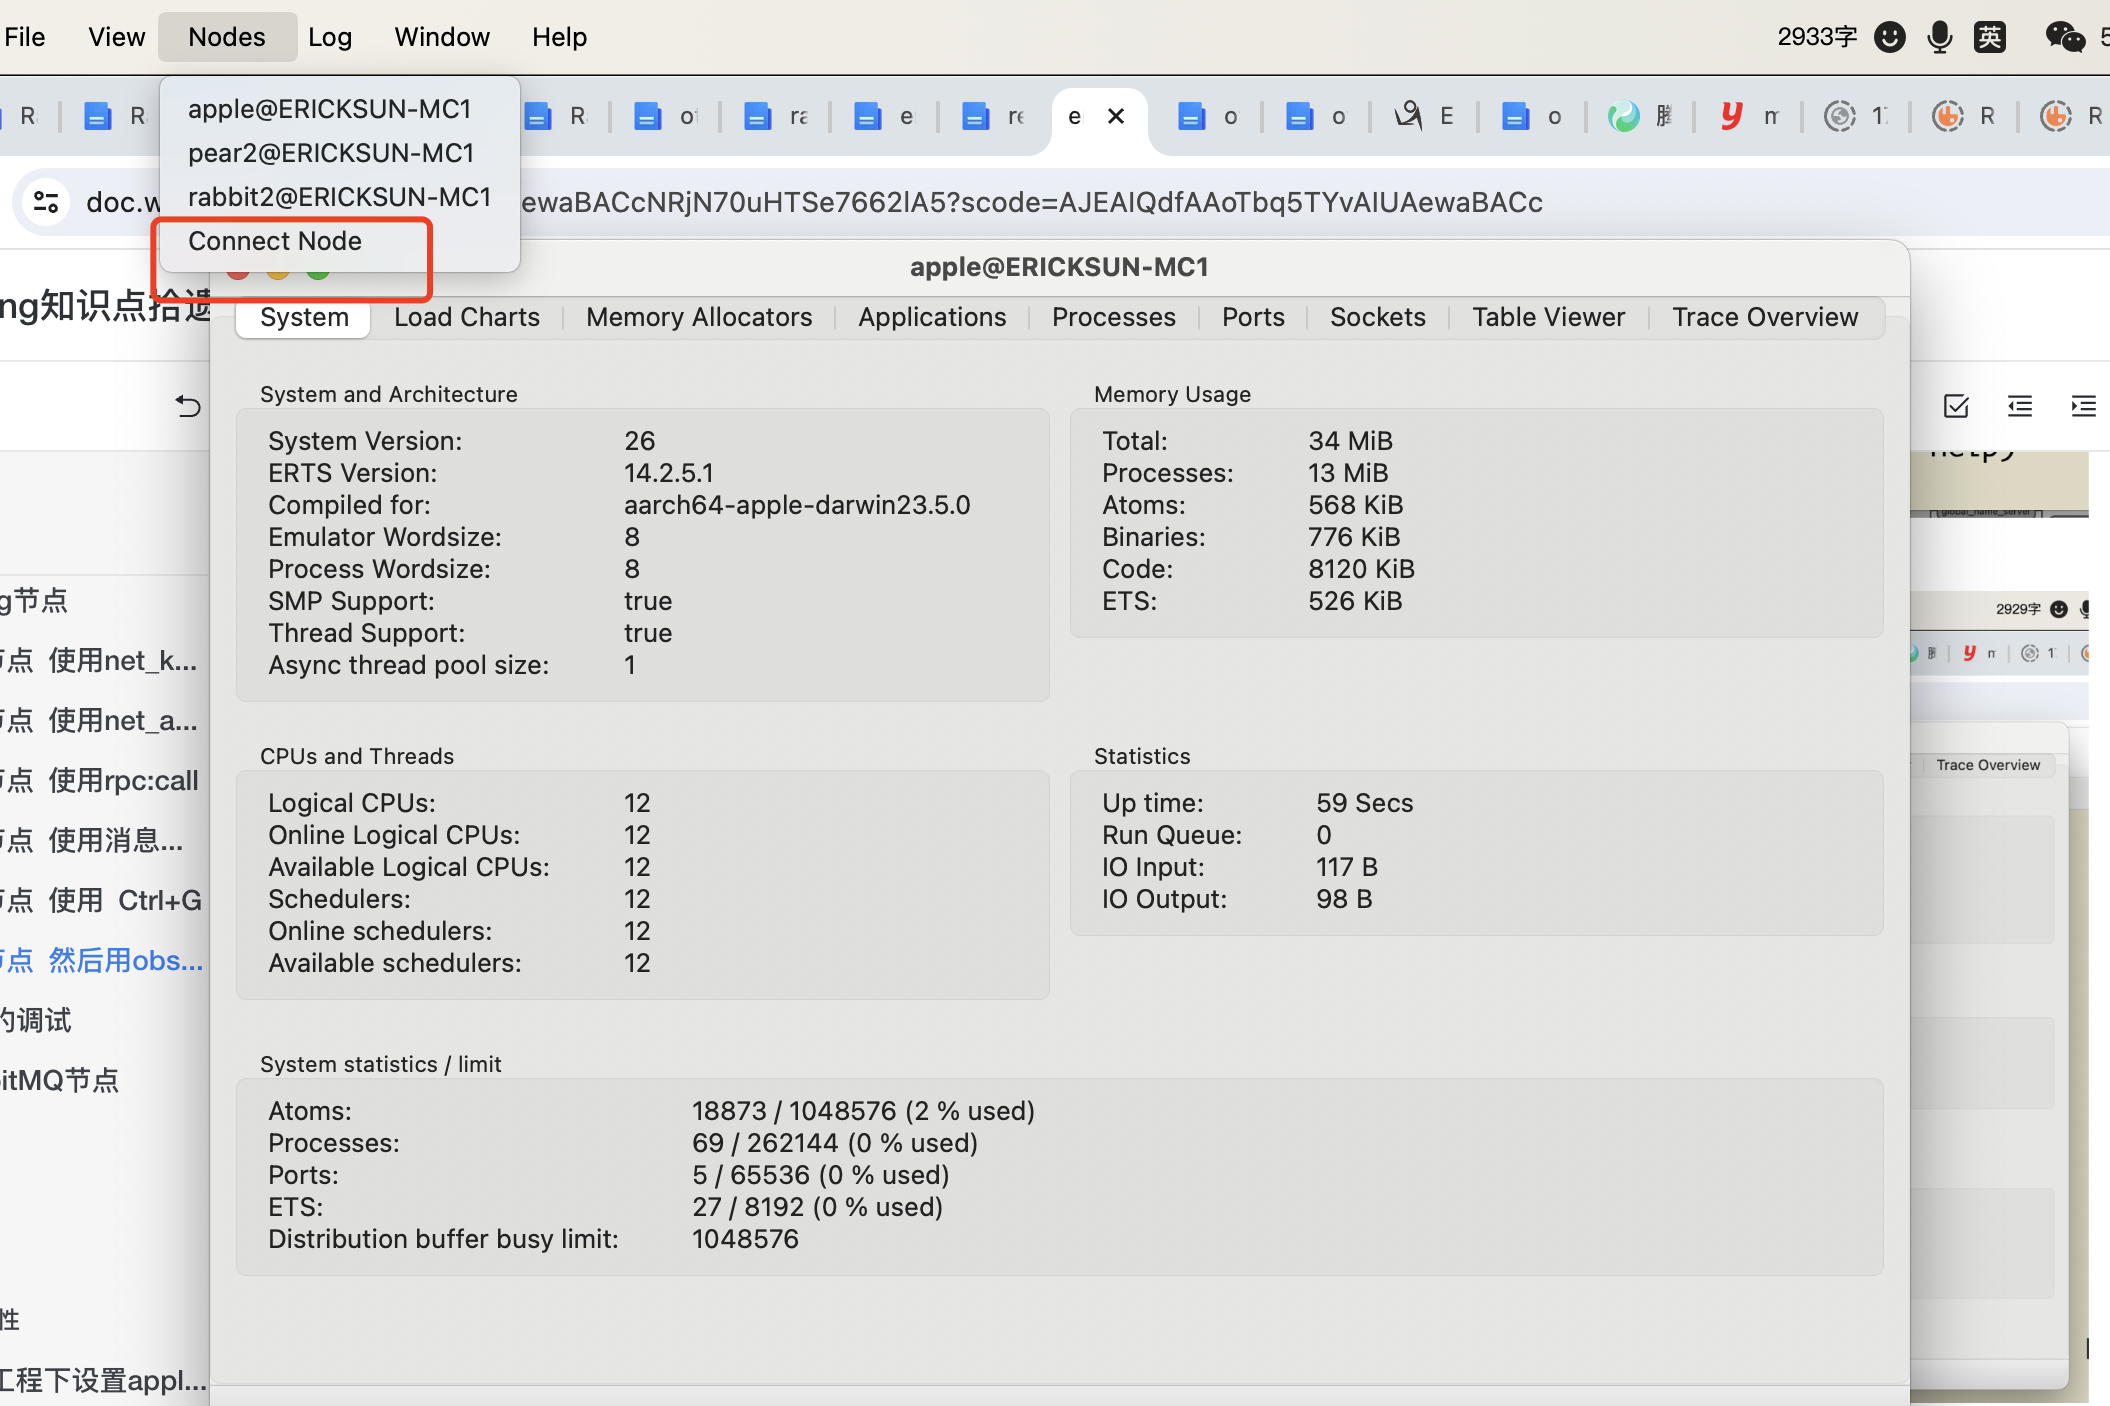
\includegraphics[width=0.85\textwidth]{image16}
\caption{连接其他节点}
\end{figure}

或者用命令行：

\begin{figure}[H]
\centering
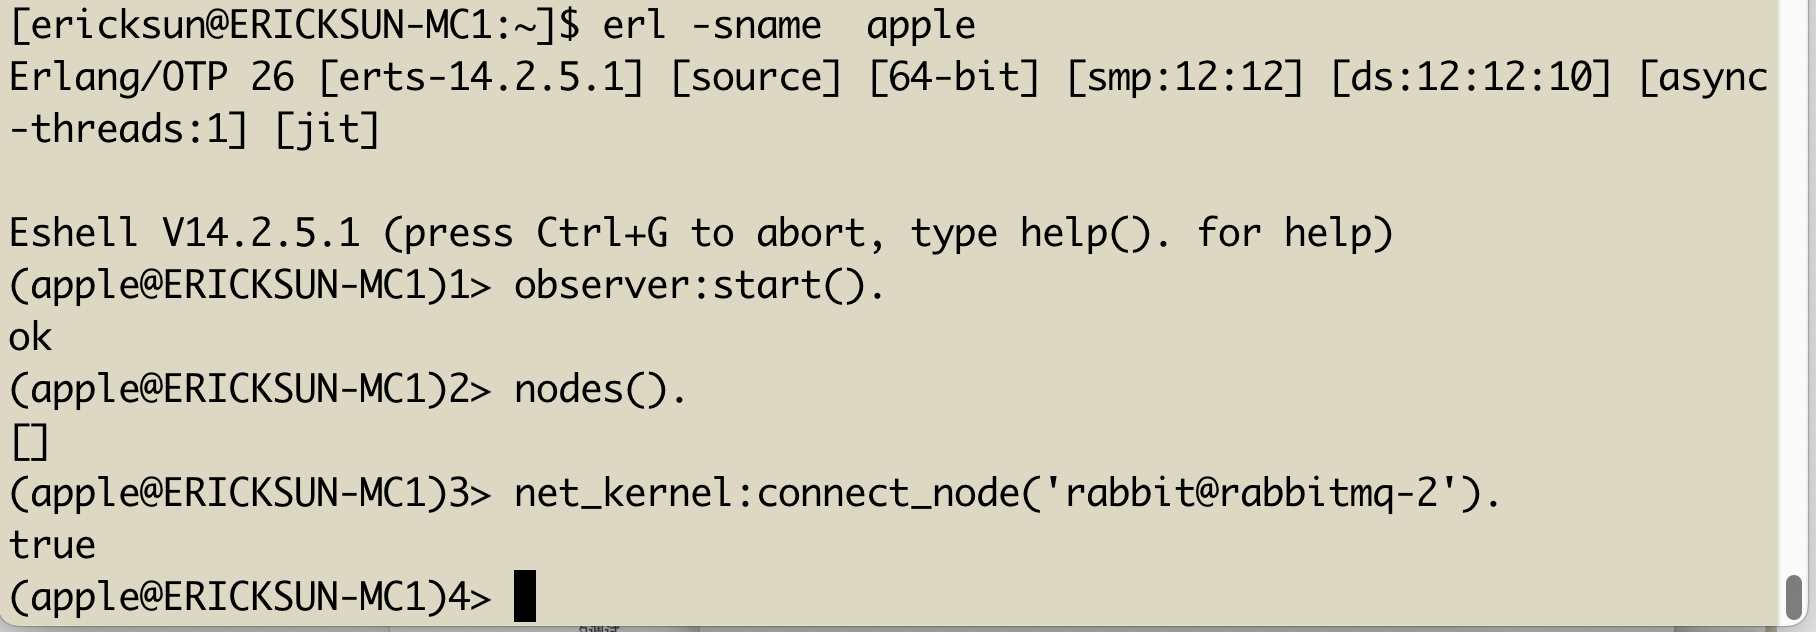
\includegraphics[width=0.85\textwidth]{image17}
\caption{命令行连接}
\end{figure}

\begin{enumerate}[leftmargin=1.5em]
    \setcounter{enumi}{3}
    \item 切换到其他节点
\end{enumerate}

\begin{figure}[H]
\centering
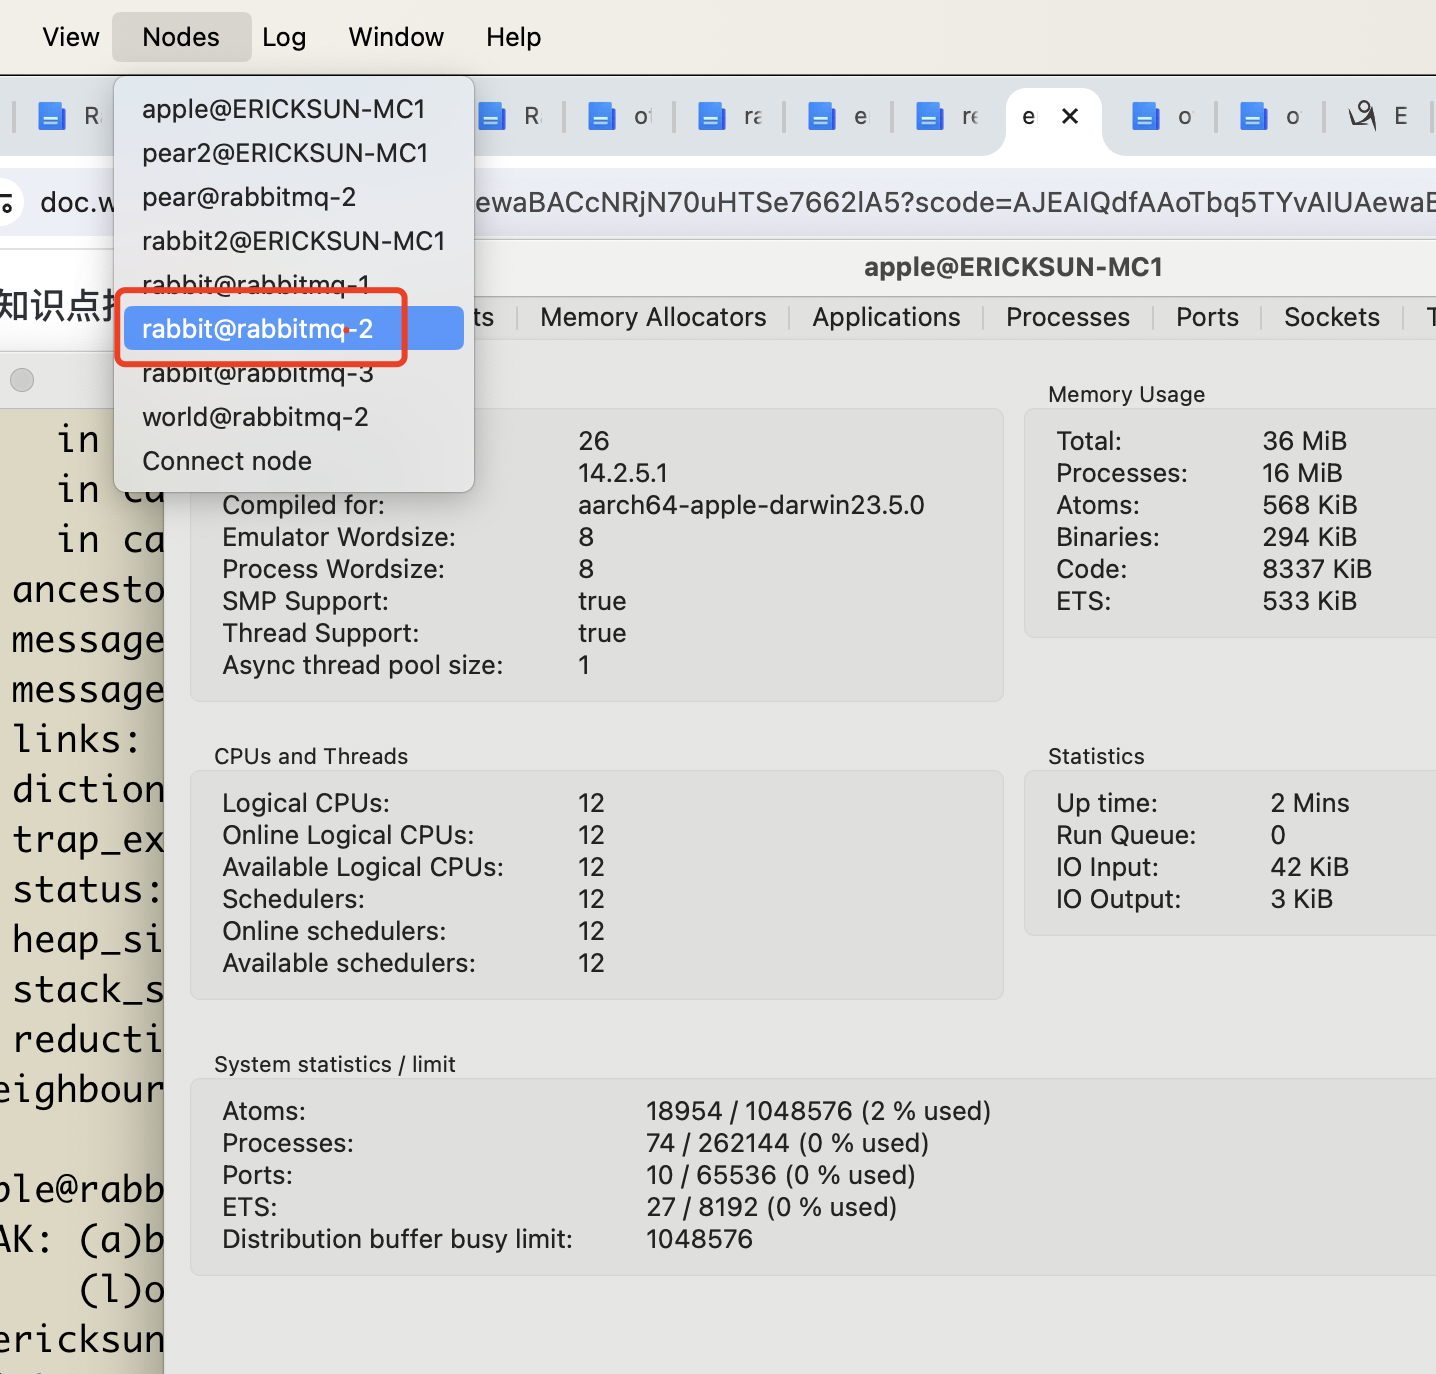
\includegraphics[width=0.85\textwidth]{image18}
\caption{切换到其他节点}
\end{figure}

\begin{enumerate}[leftmargin=1.5em]
    \setcounter{enumi}{4}
    \item 查看节点信息
\end{enumerate}

\begin{figure}[H]
\centering
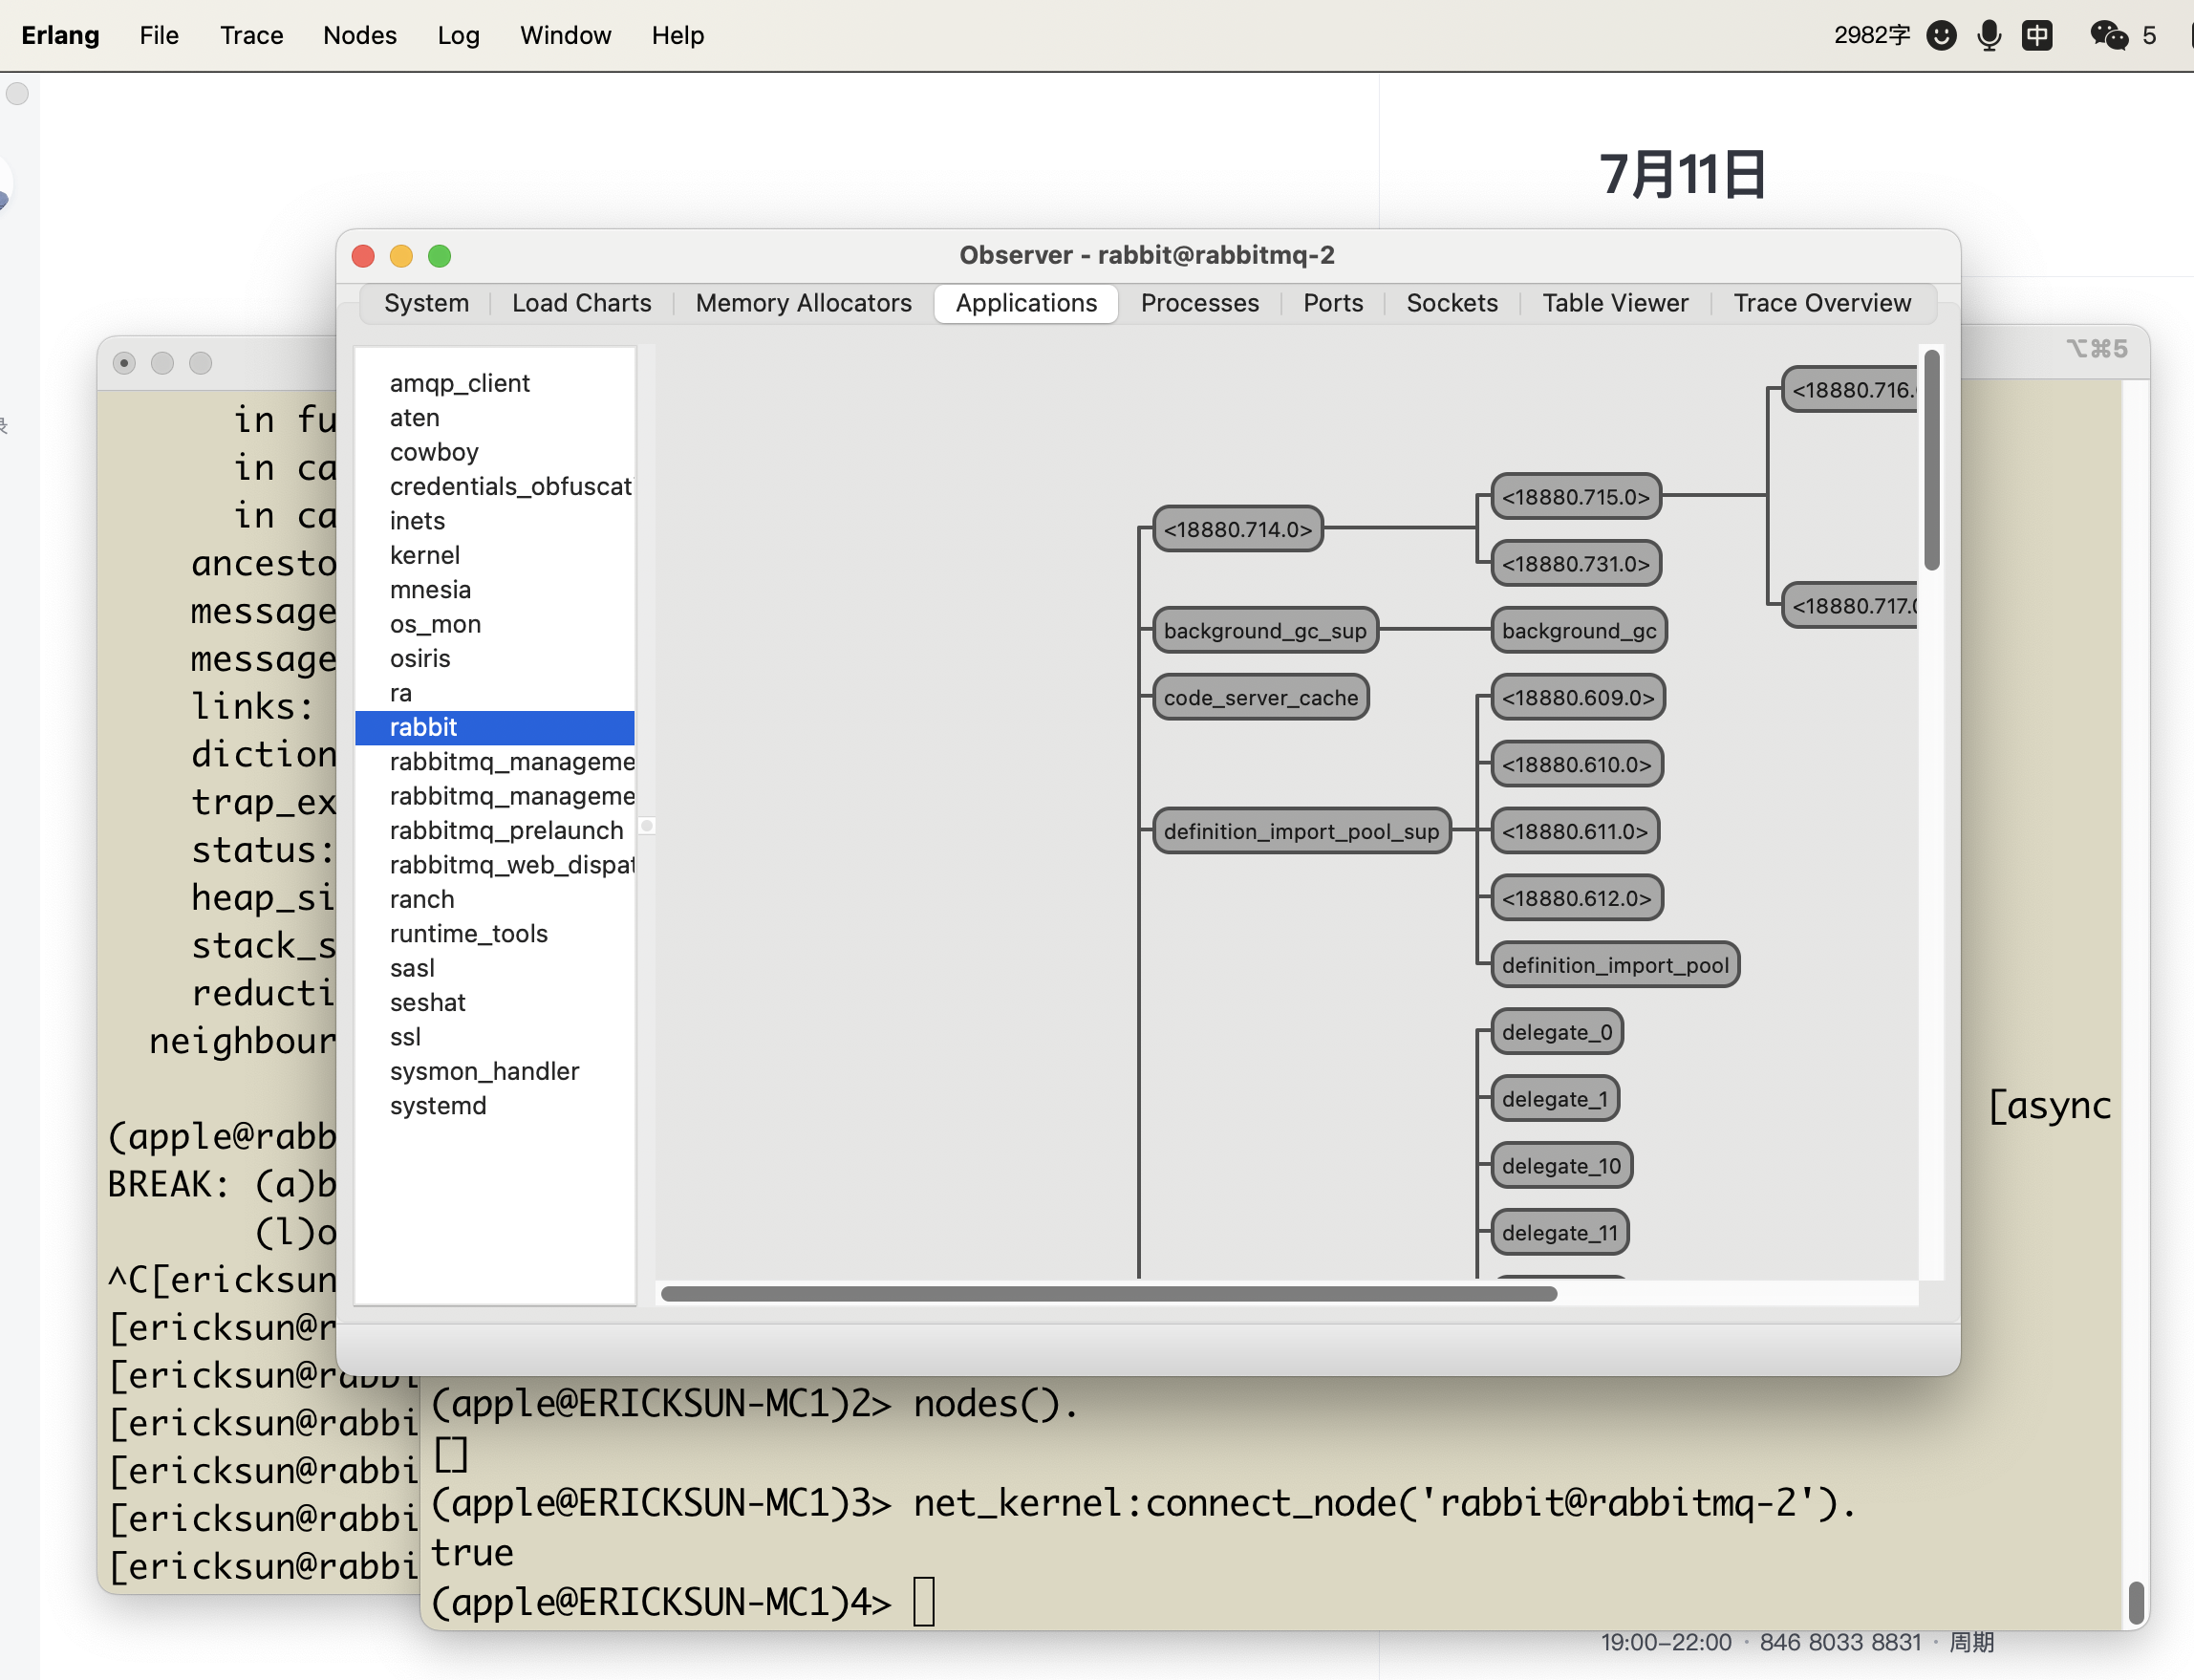
\includegraphics[width=0.85\textwidth]{image19}
\caption{节点信息}
\end{figure}

\subsection{节点无法连接的调试}

\begin{itemize}[leftmargin=1.5em]
    \item 查看防火墙，如果有，需要关闭
    \item 检查 \lstinline|.erlang.cookie| 是否一致
    \item 检查 hosts 配置
\end{itemize}

\begin{figure}[H]
\centering
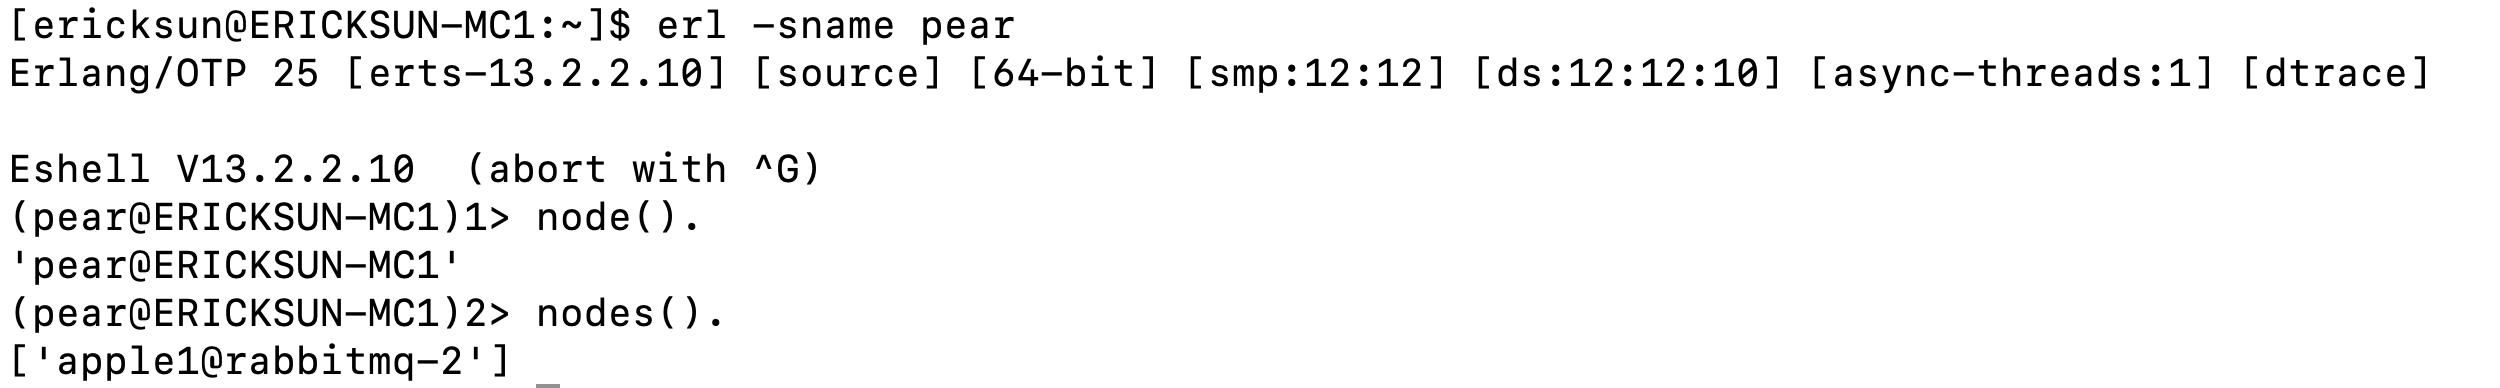
\includegraphics[width=0.85\textwidth]{image20}
\caption{节点连接调试 (1)}
\end{figure}

\begin{figure}[H]
\centering
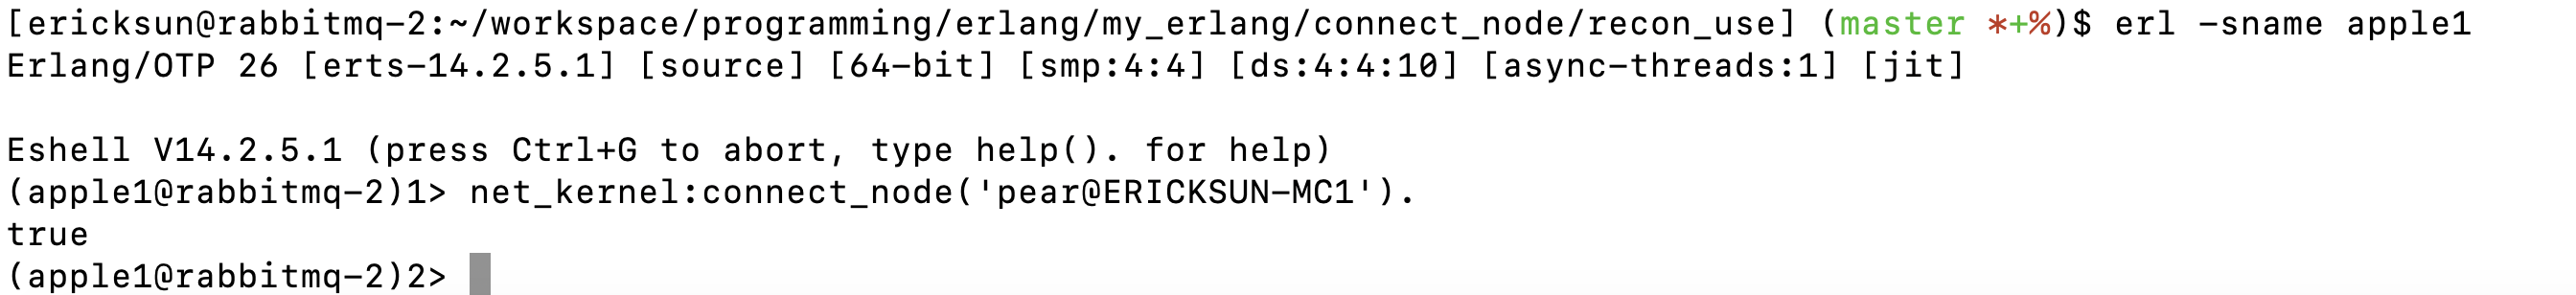
\includegraphics[width=0.85\textwidth]{image21}
\caption{节点连接调试 (2)}
\end{figure}

\begin{figure}[H]
\centering
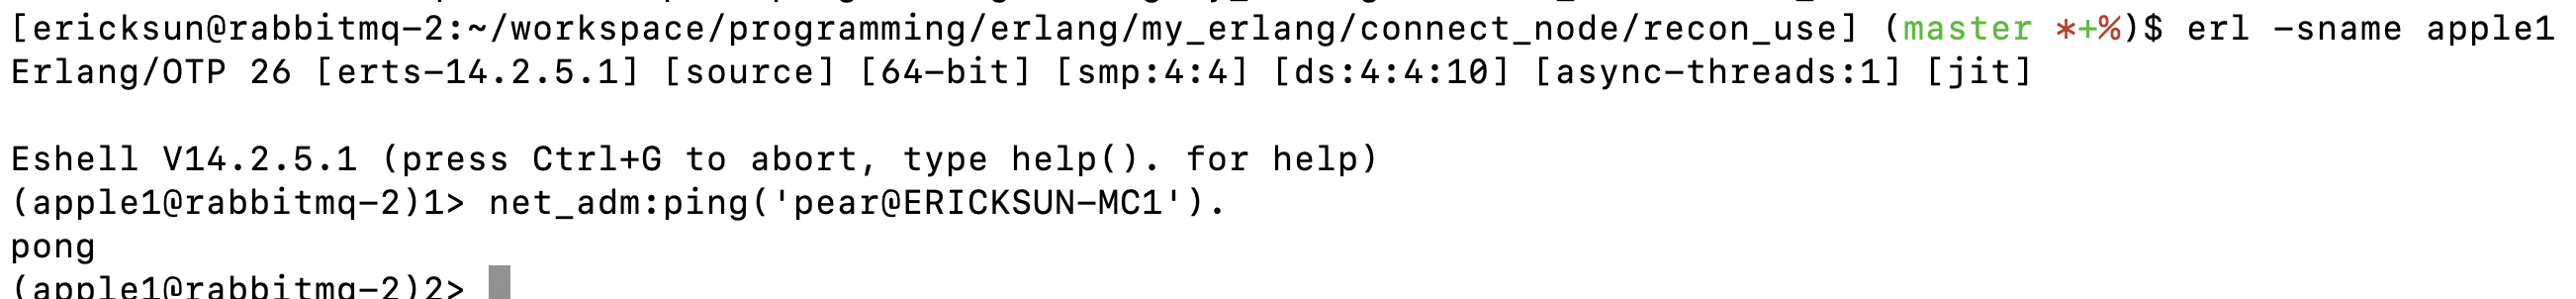
\includegraphics[width=0.85\textwidth]{image22}
\caption{节点连接调试 (3)}
\end{figure}

\subsection{把一个节点变成分布式节点}

为节点起名字即可：

\begin{lstlisting}
net_kernel:start([foo, shortnames]).
\end{lstlisting}

启动之前：

\begin{figure}[H]
\centering
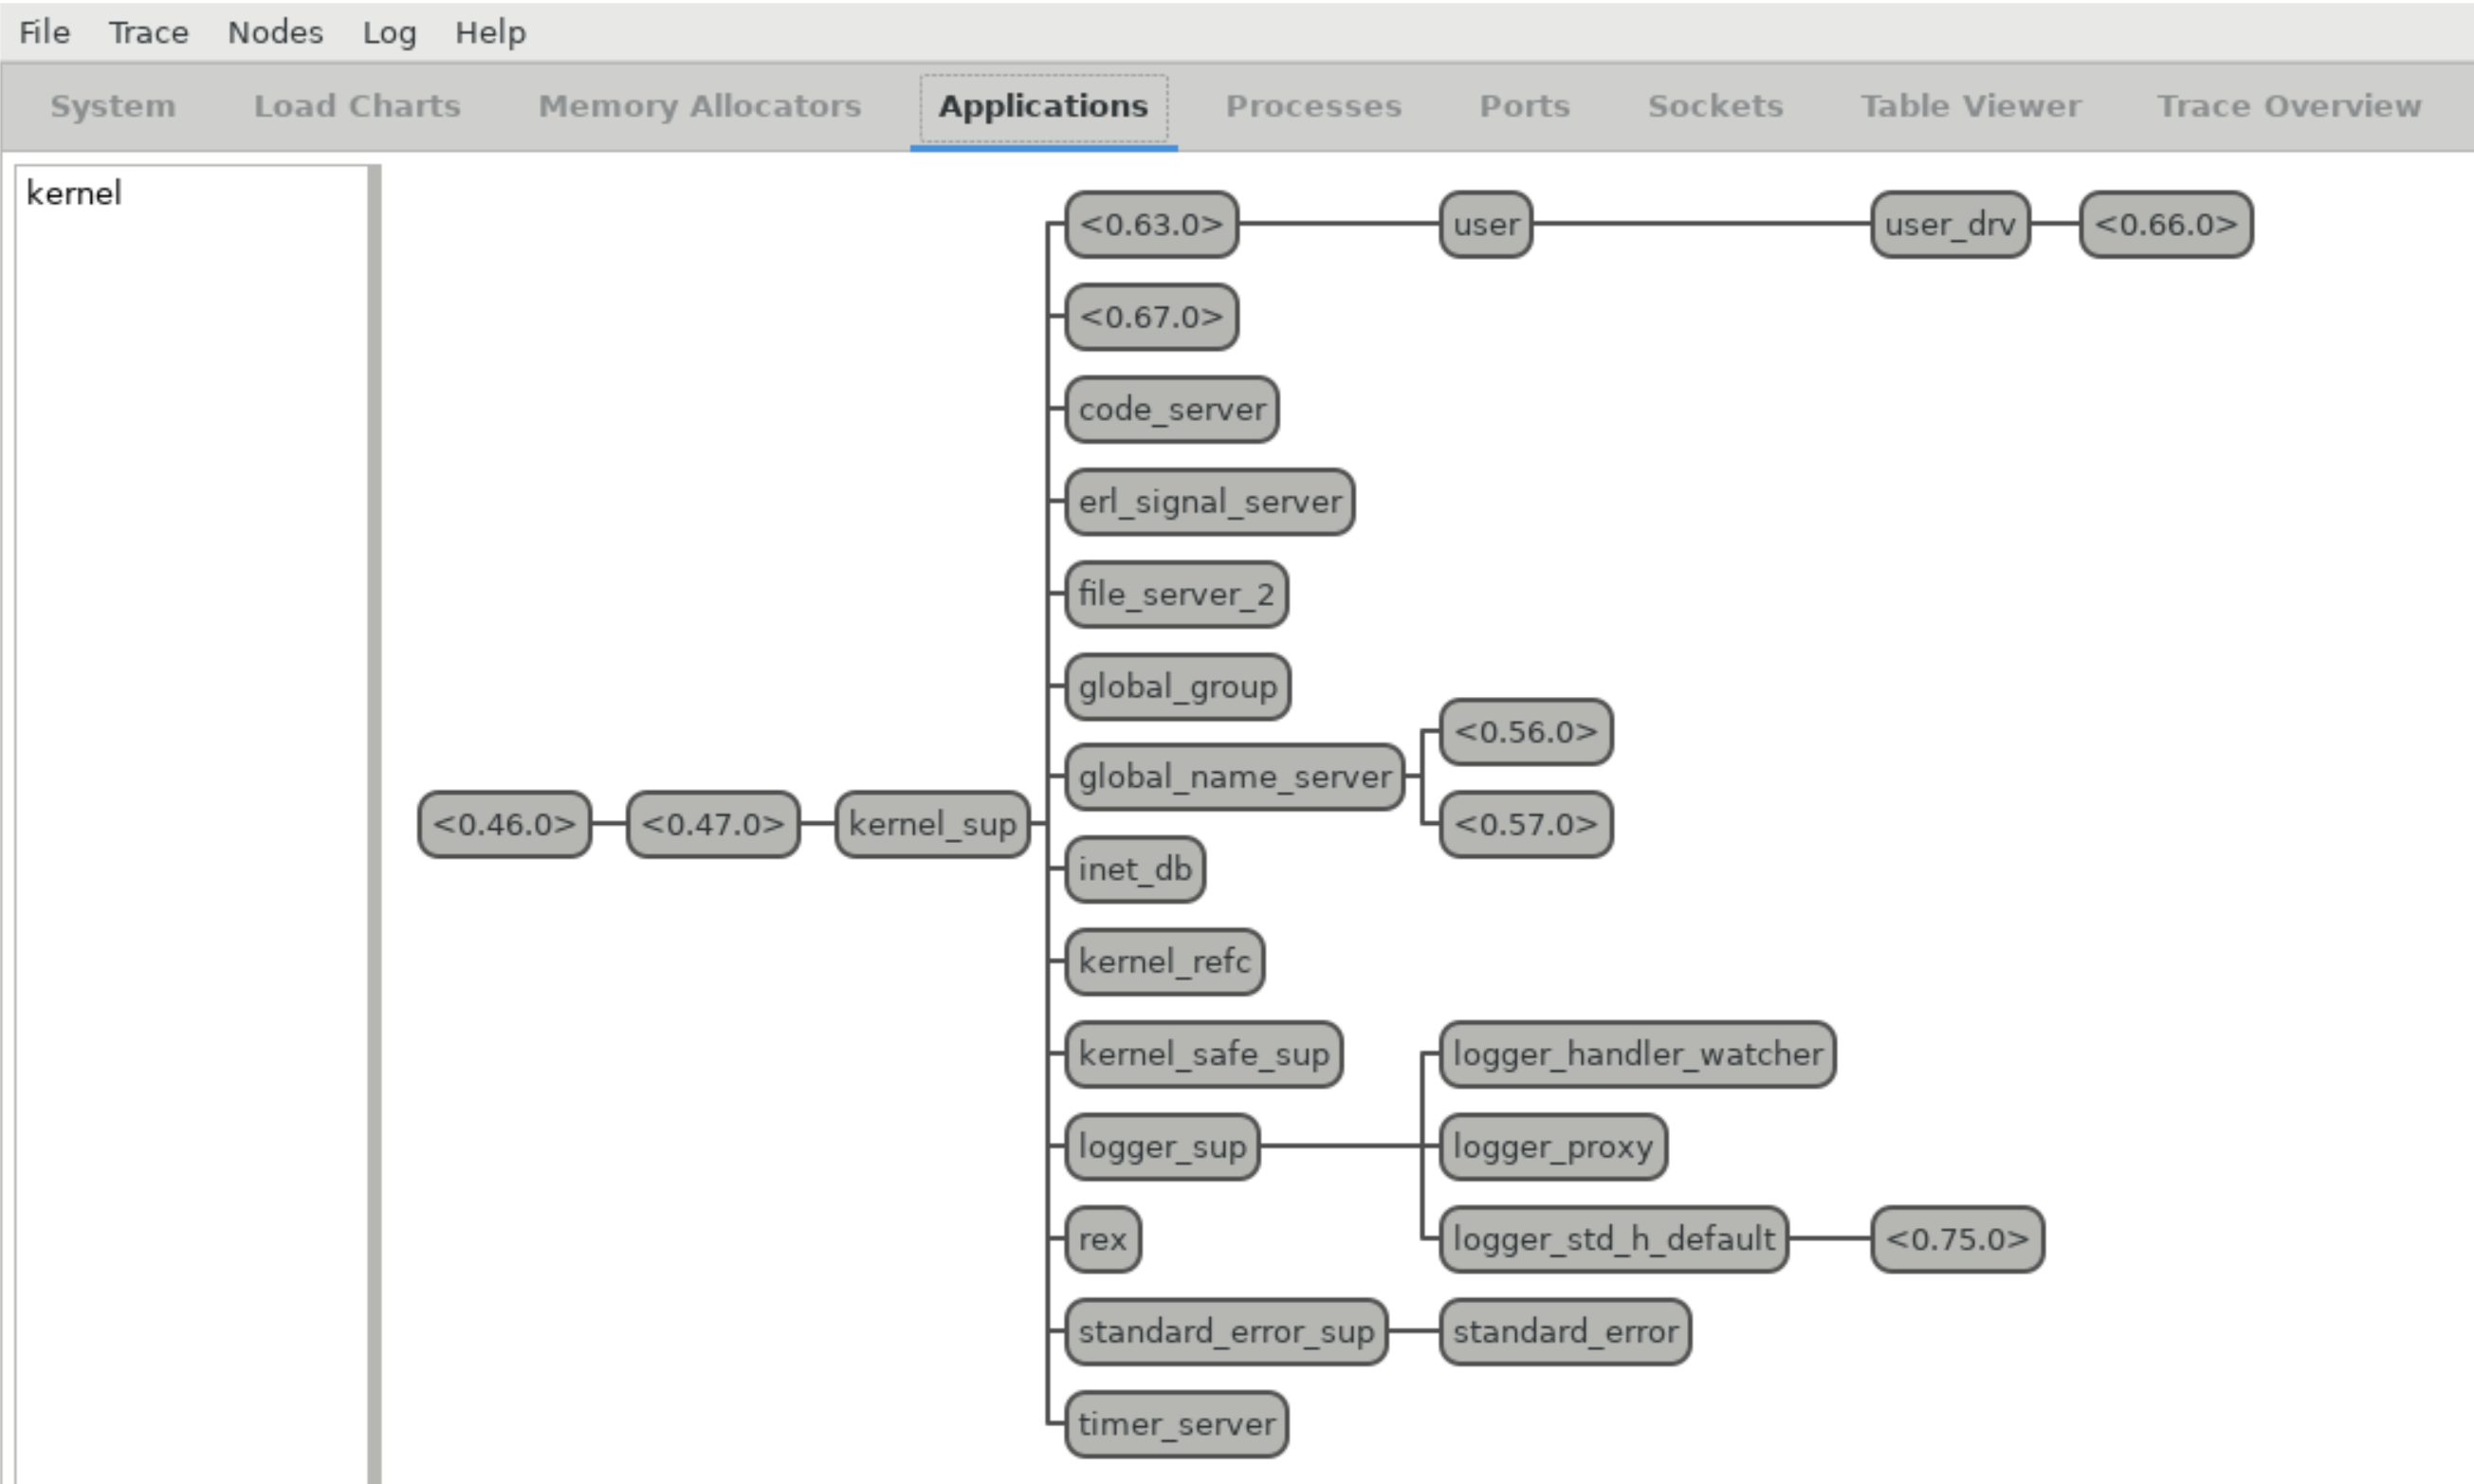
\includegraphics[width=0.6\textwidth]{image30}
\caption{启动分布式之前}
\end{figure}

启动之后：

\begin{figure}[H]
\centering
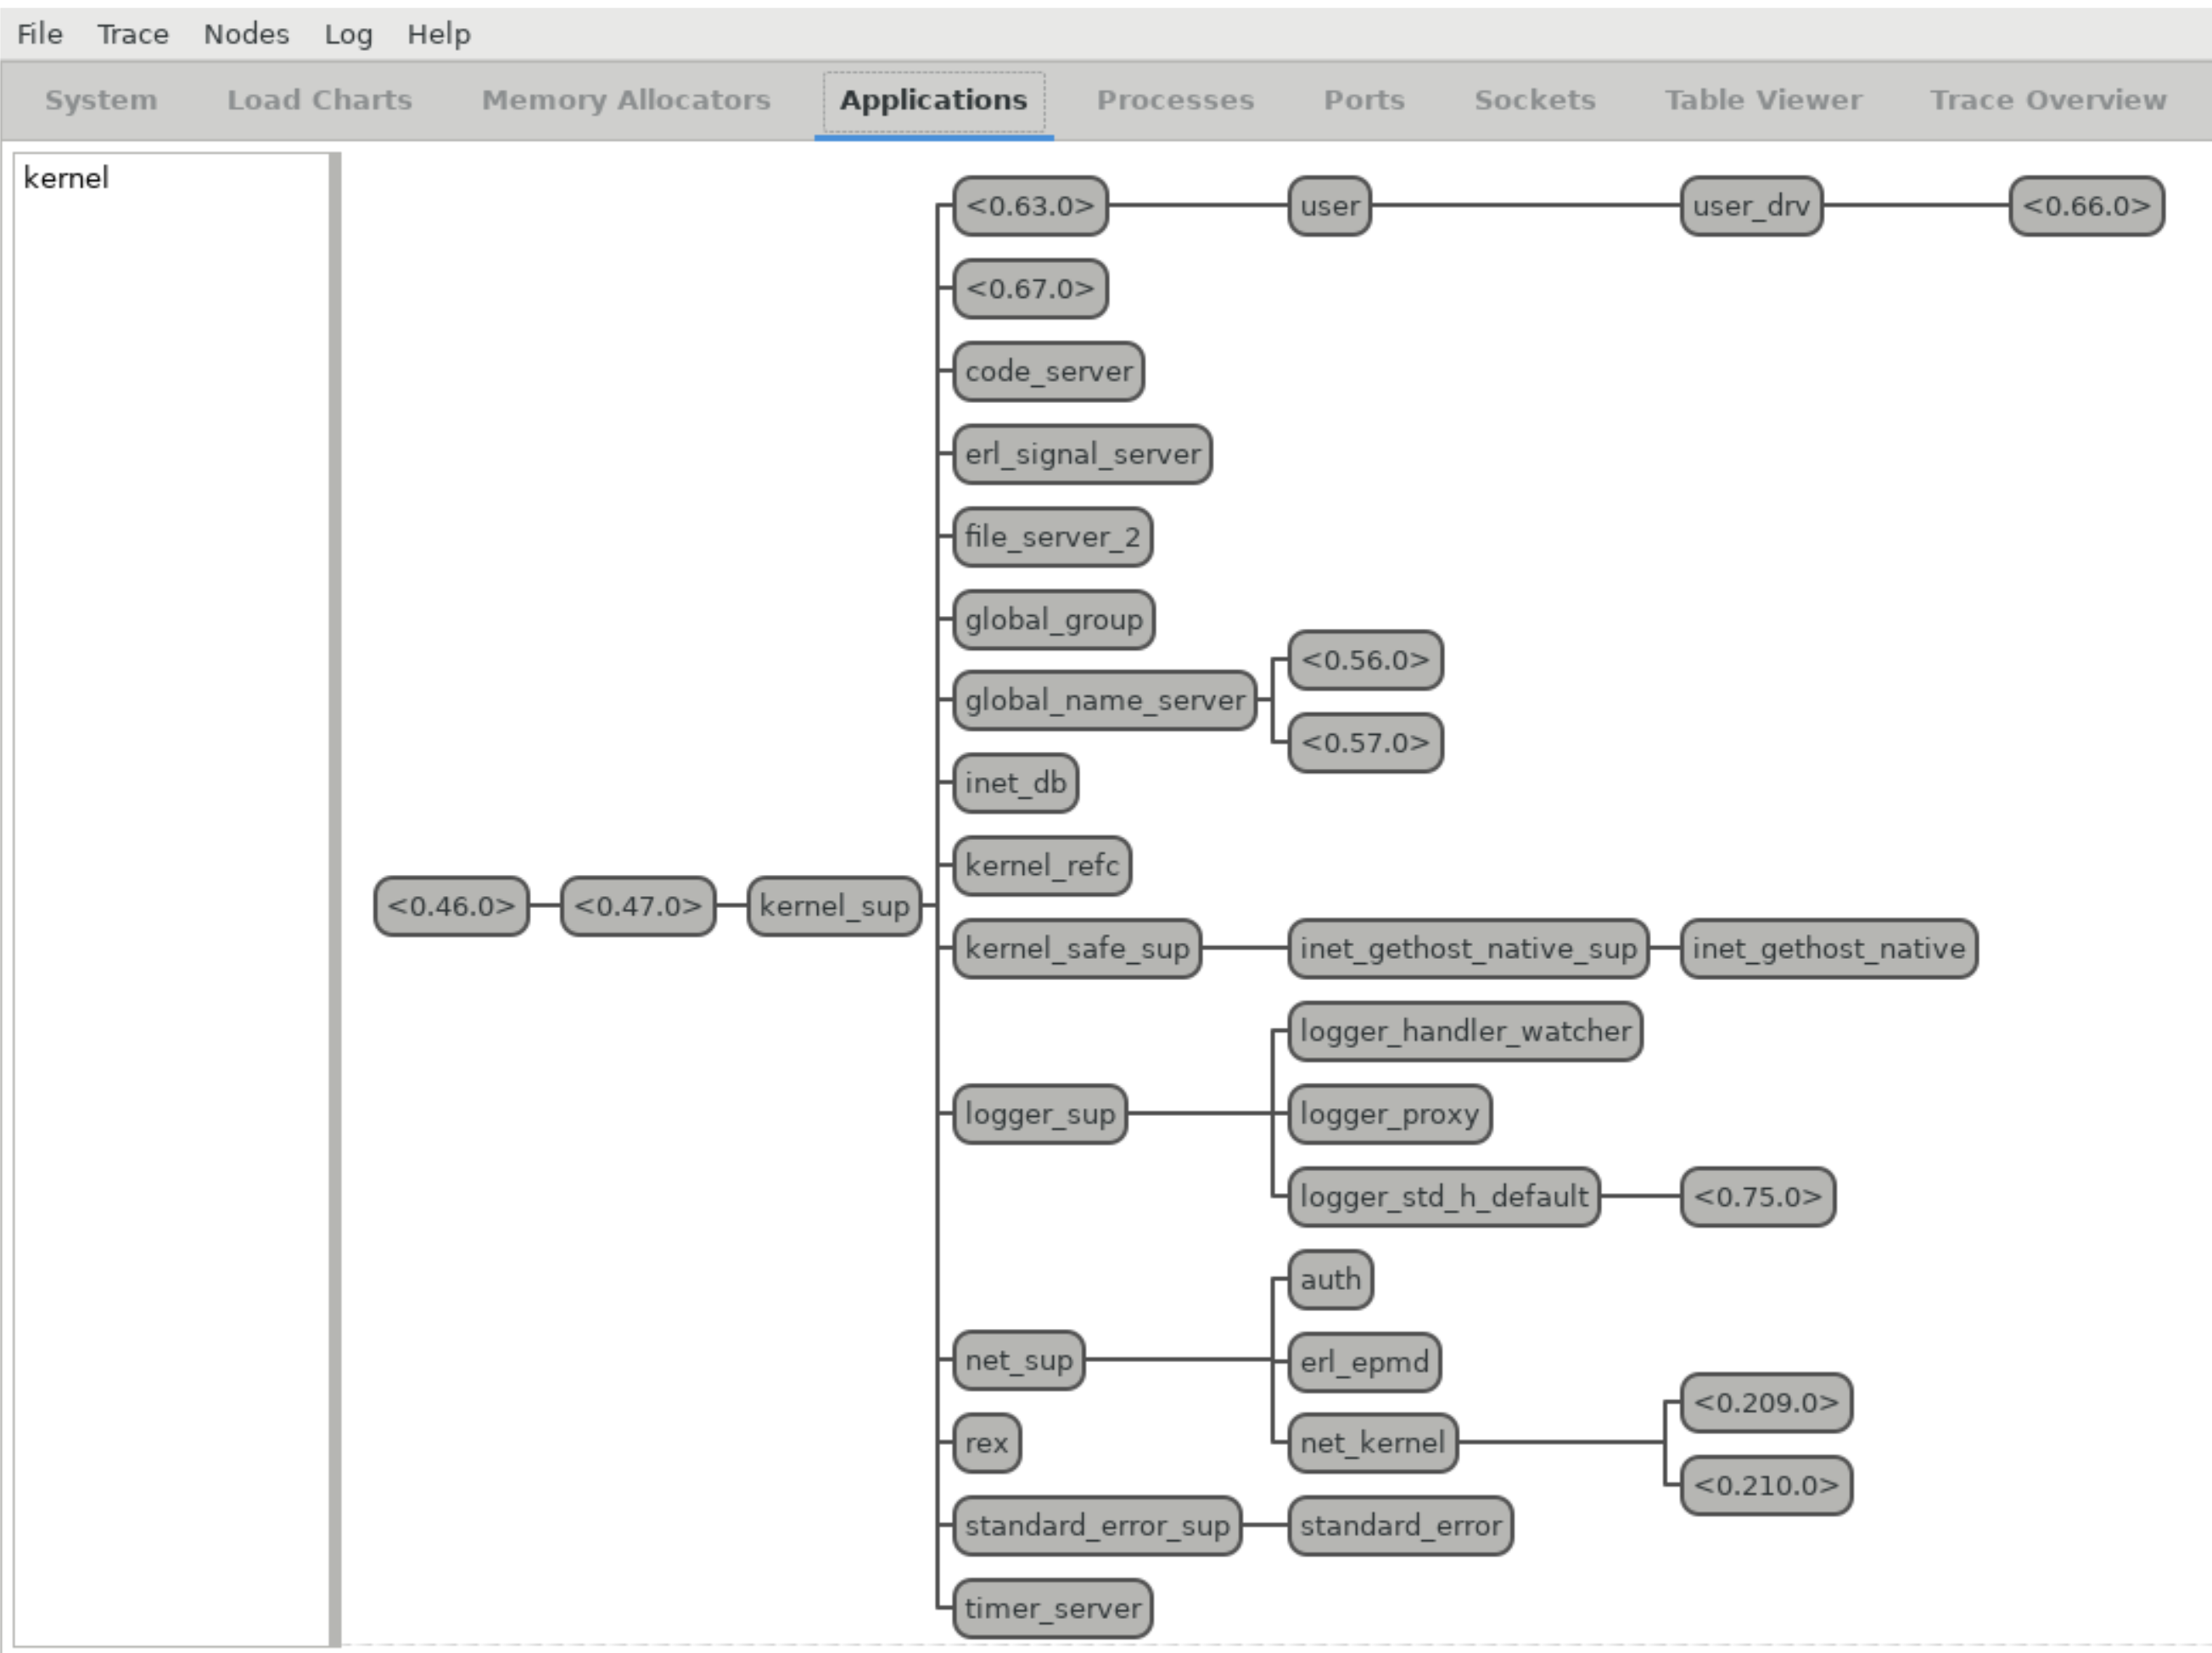
\includegraphics[width=0.6\textwidth]{image31}
\caption{启动分布式之后}
\end{figure}

\begin{figure}[H]
\centering
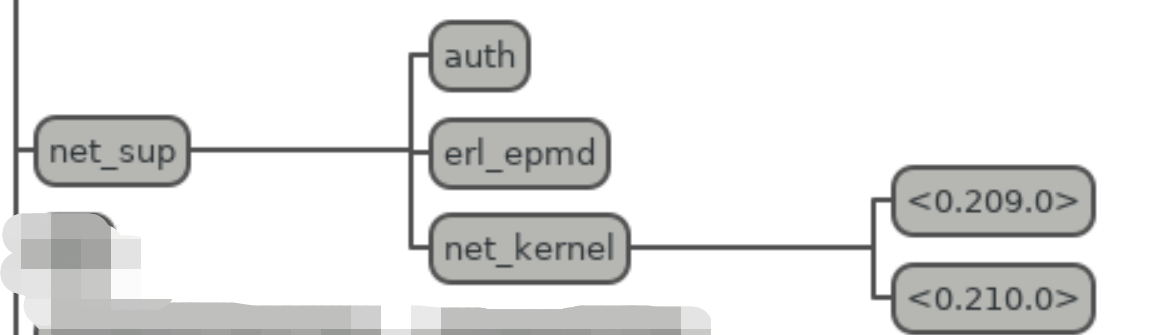
\includegraphics[width=0.85\textwidth]{image32}
\caption{net\_kernel:start 结果}
\end{figure}

这是多出来的一部分：

\begin{figure}[H]
\centering
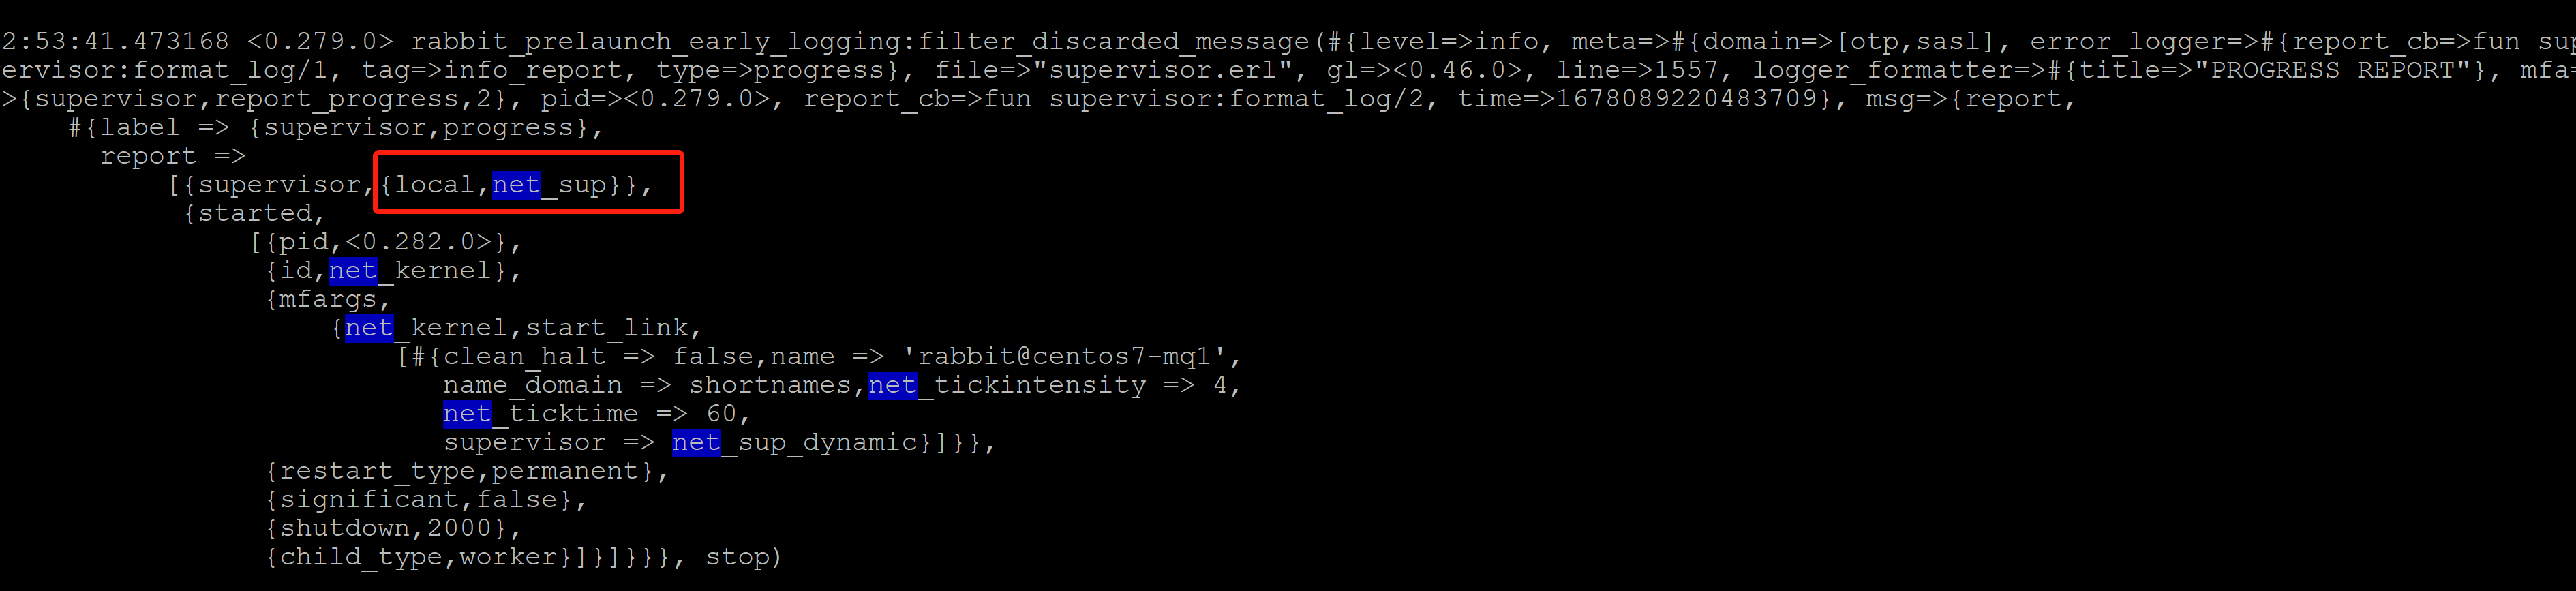
\includegraphics[width=0.85\textwidth]{image33}
\caption{新增部分 (1)}
\end{figure}

\begin{figure}[H]
\centering
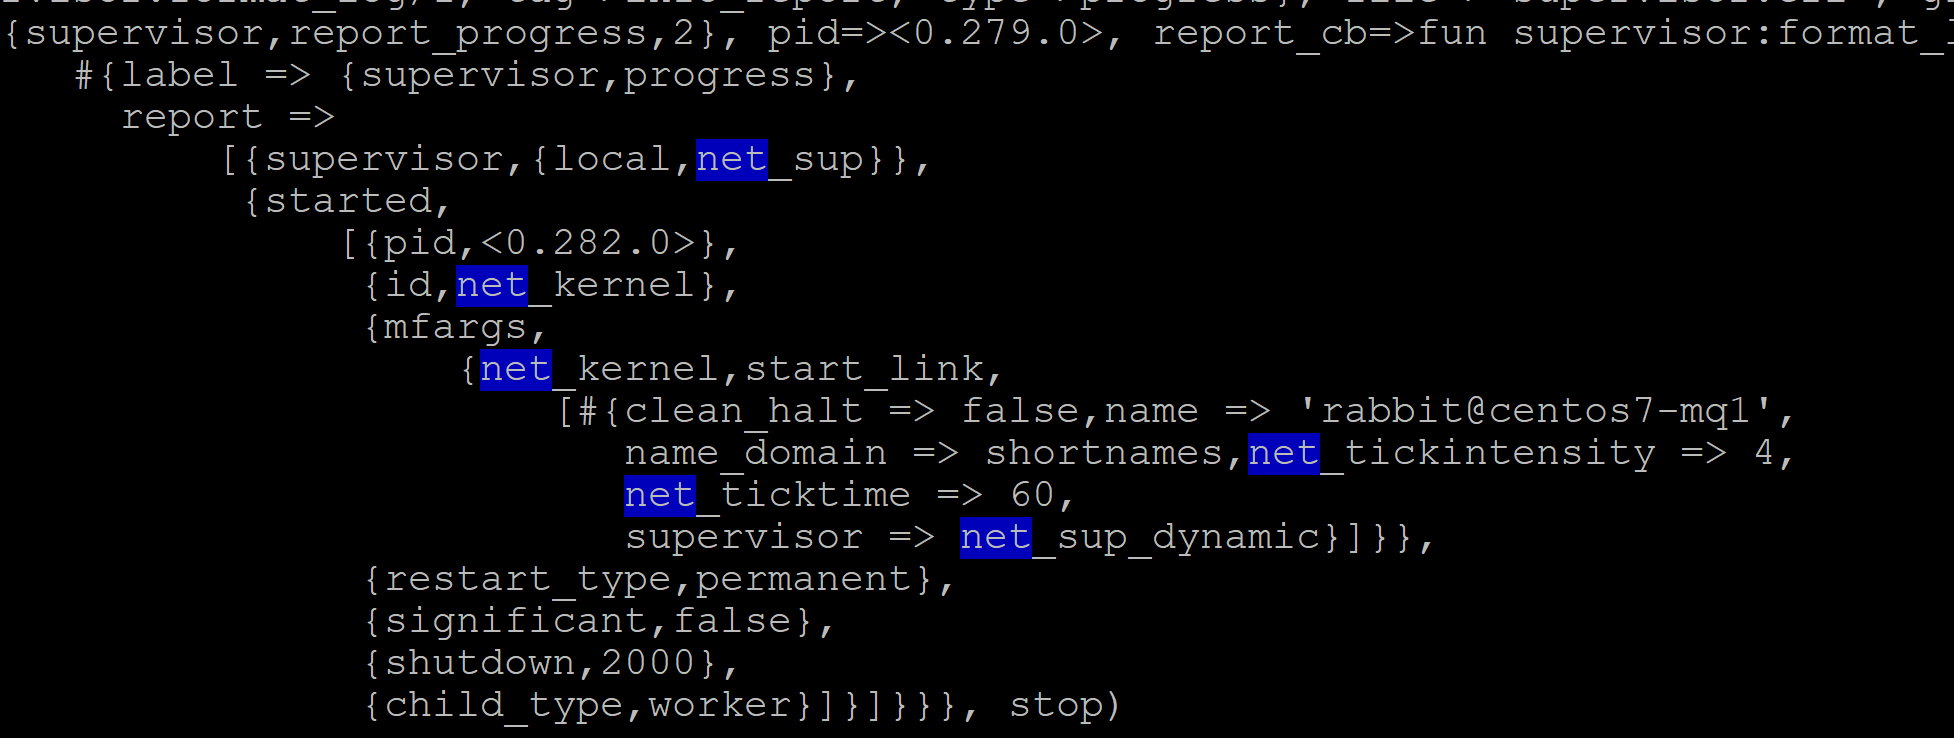
\includegraphics[width=0.85\textwidth]{image34}
\caption{新增部分 (2)}
\end{figure}

源码位置：\lstinline|kernel-8.4.2/src/erl_distribution.erl|

\begin{figure}[H]
\centering
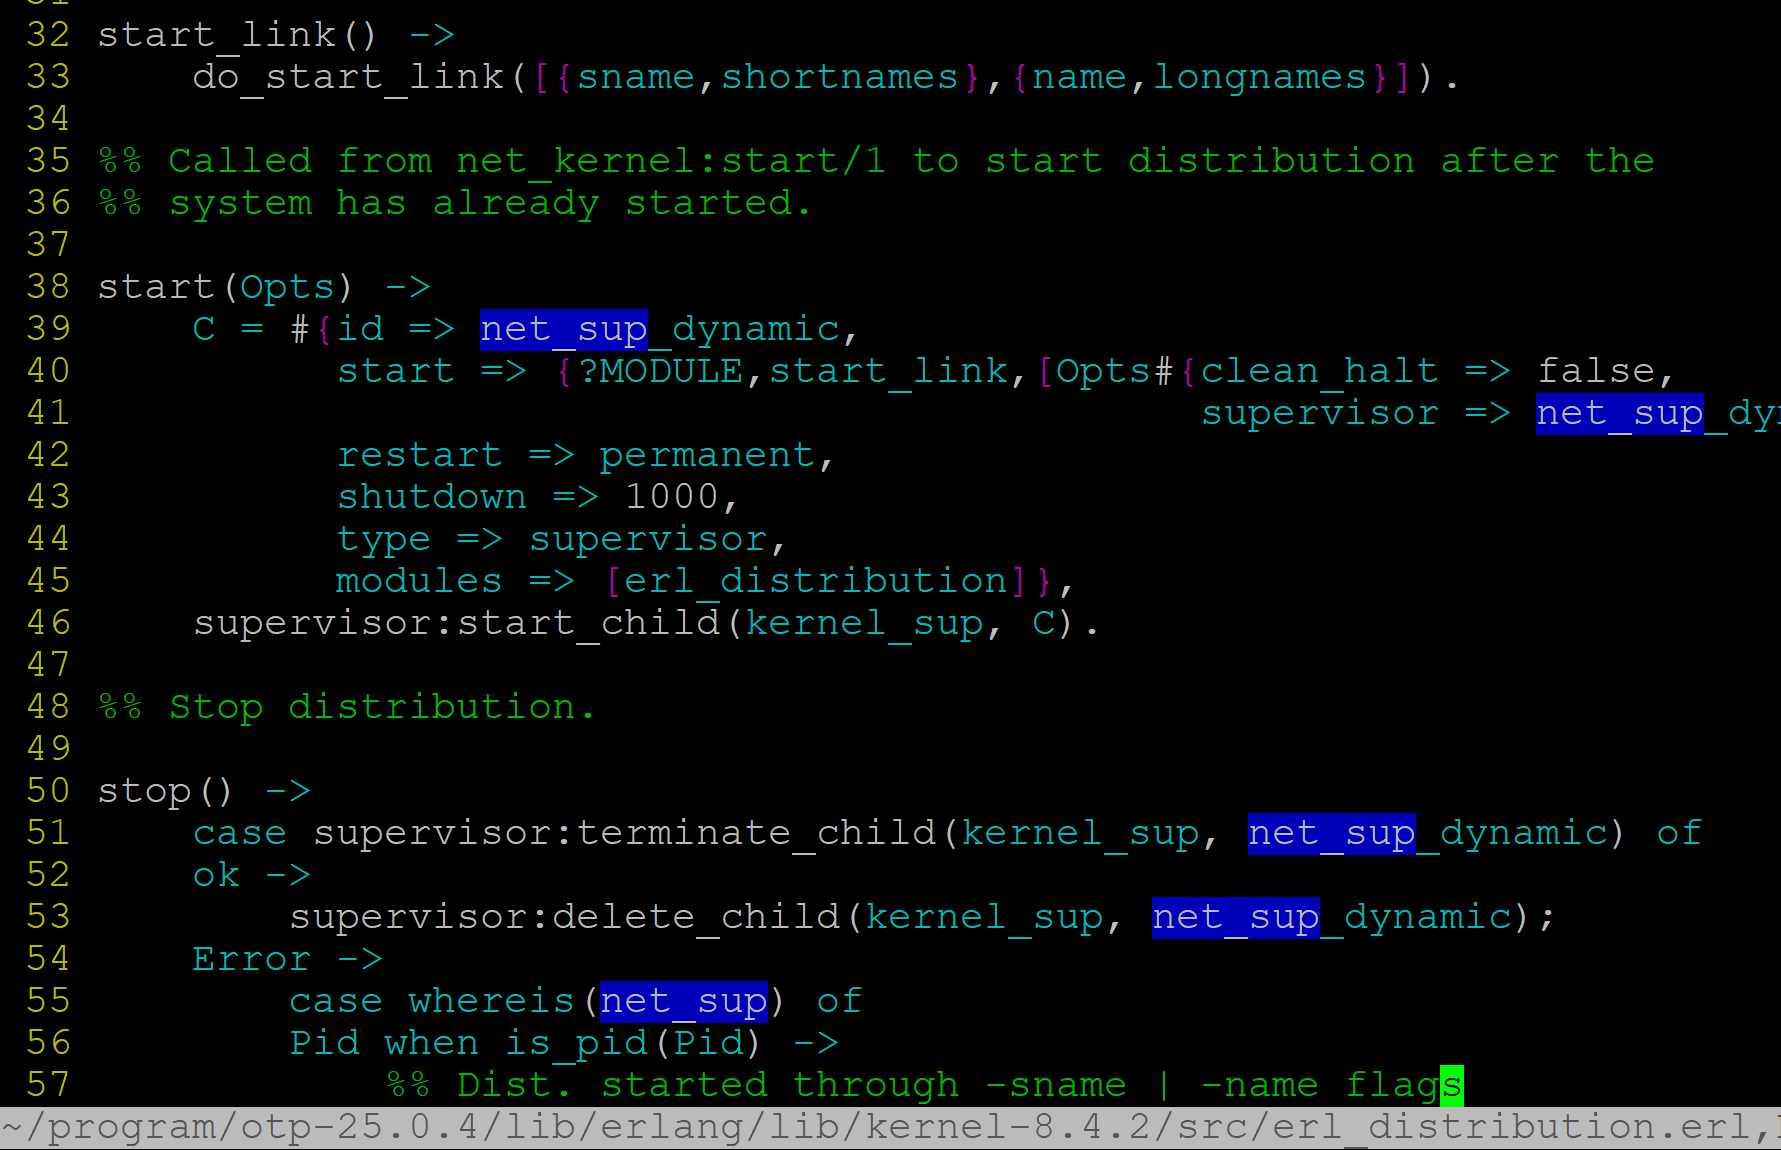
\includegraphics[width=0.85\textwidth]{image35}
\caption{erl\_distribution 源码 (1)}
\end{figure}

\begin{figure}[H]
\centering
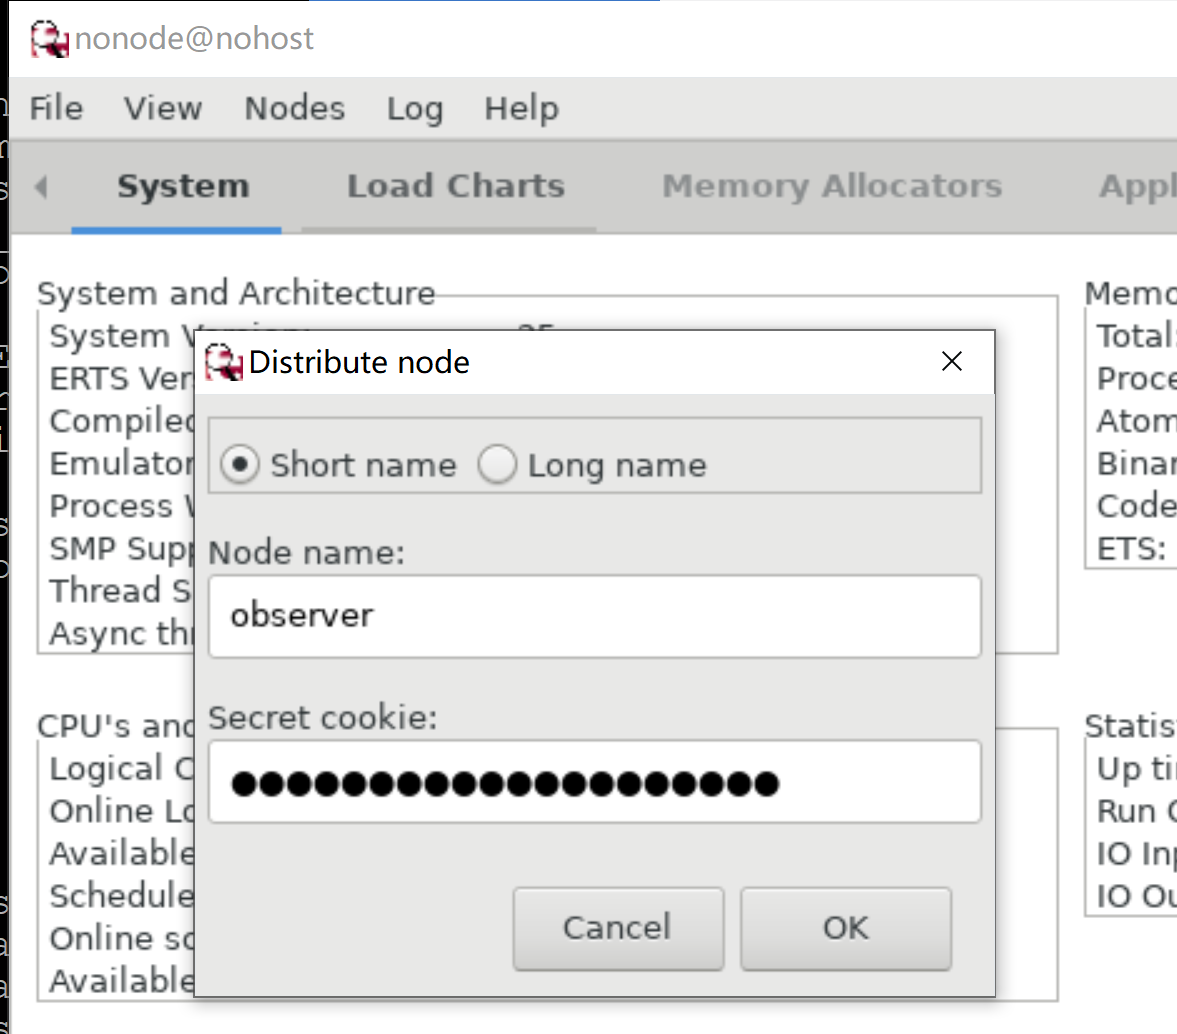
\includegraphics[width=0.85\textwidth]{image36}
\caption{erl\_distribution 源码 (2)}
\end{figure}

\subsection{Erlang 节点间通信}

参见：\href{https://doc.weixin.qq.com/doc/w3_AIUAewaBACcKvp9d0QlSbafbqP8YO?scode=AJEAIQdfAAo4VWNB0wAIUAewaBACc}{erlang 节点间通信 -- Net Tick Time}

\subsection{找到 pid/reference/port 所在的 node}

参考：\href{https://www.erlang.org/doc/man/erlang.html#node-1}{Erlang -- erlang:node/1}

% ============================================================
% Section 4: Debugging and Monitoring
% ============================================================
\section{调试与监控}

\subsection{调试 RabbitMQ 节点}

\subsubsection{初步启动}

\begin{figure}[H]
\centering
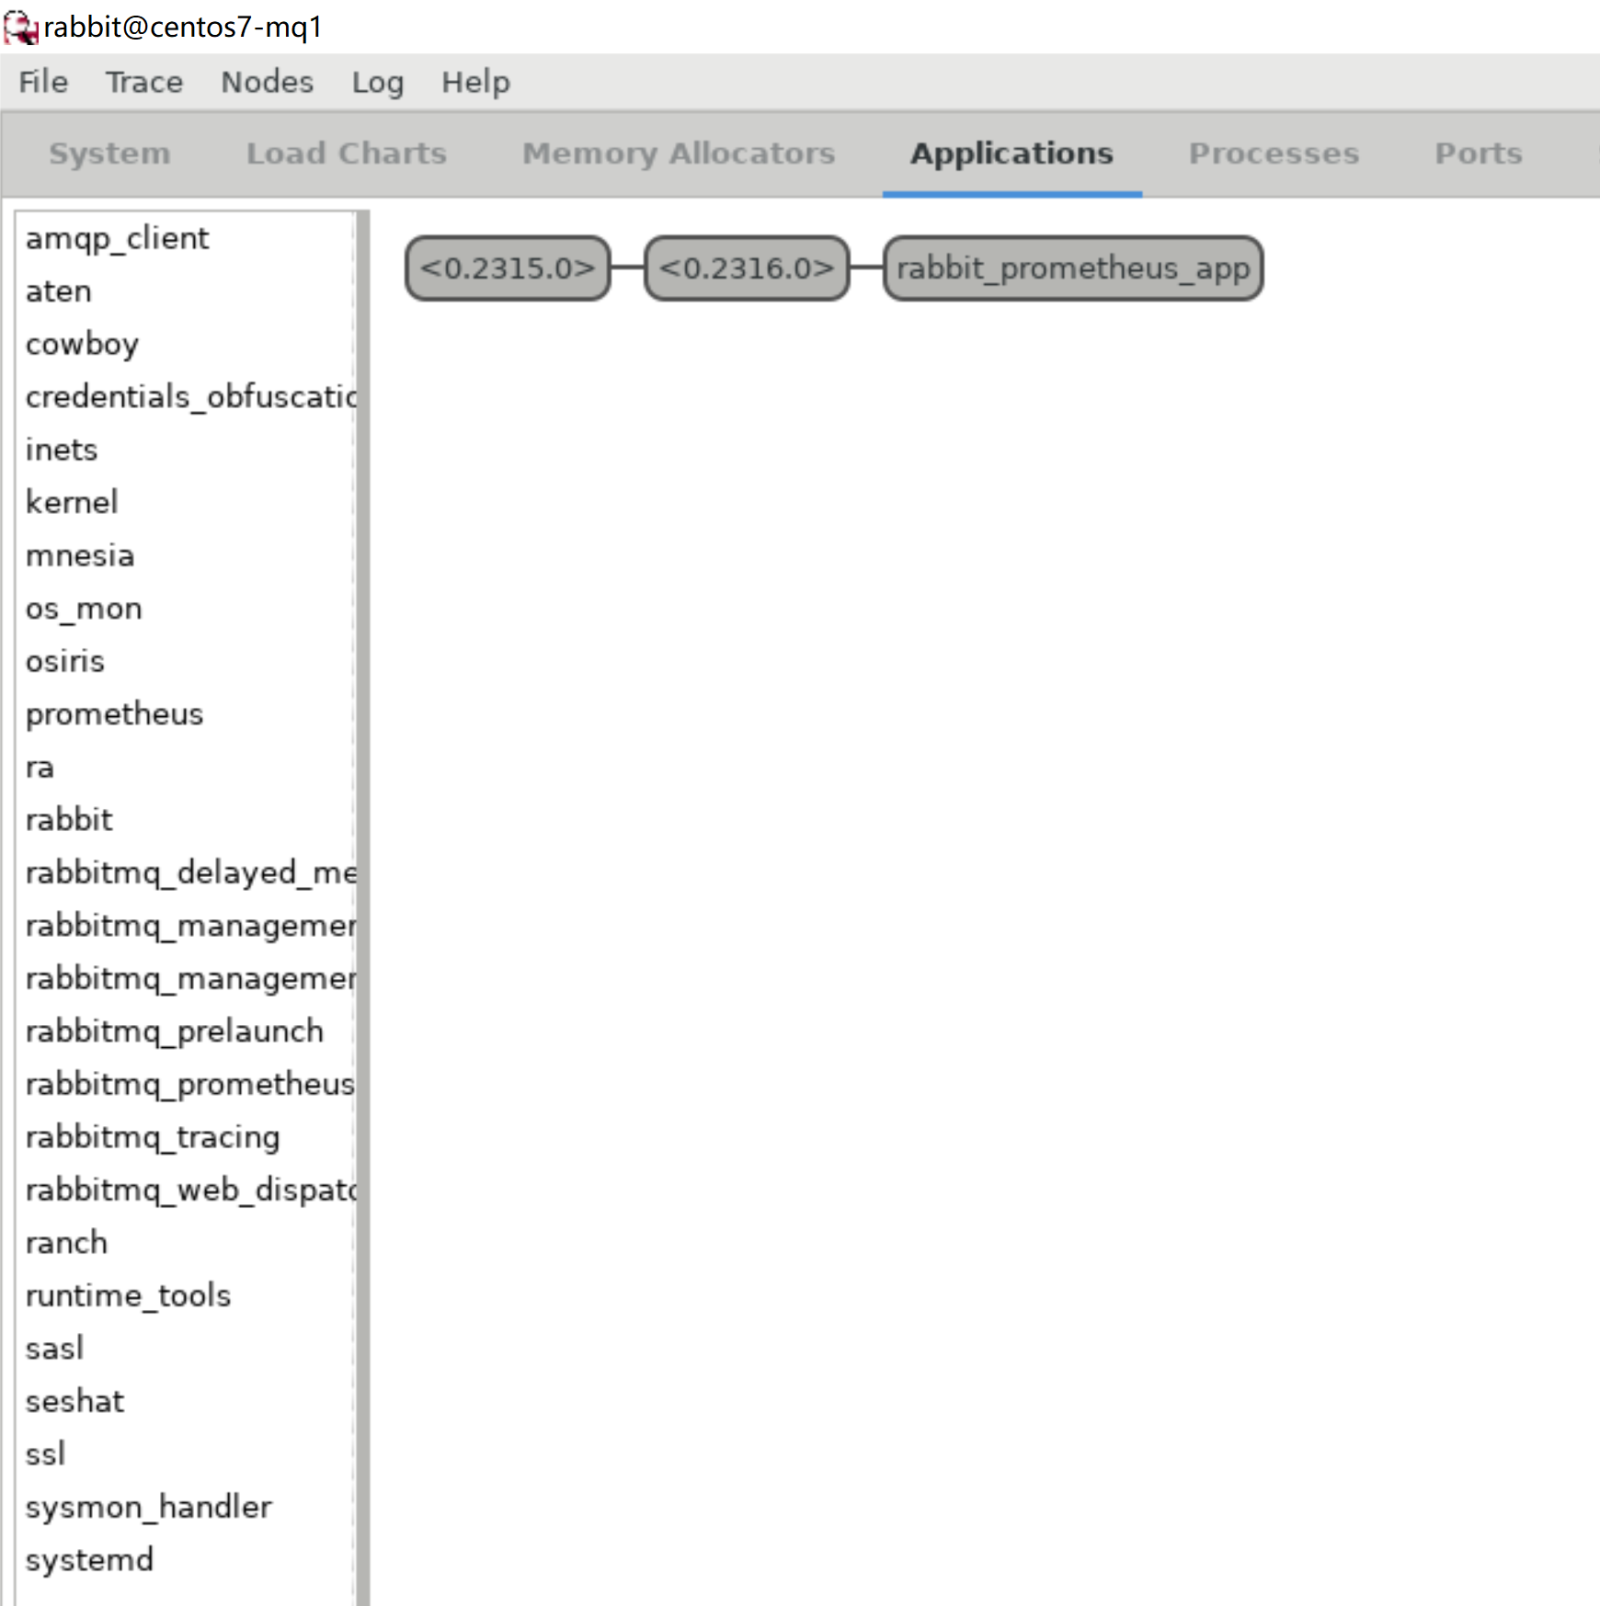
\includegraphics[width=0.35\textwidth]{image23}
\caption{RabbitMQ 初步启动}
\end{figure}

\subsubsection{停止}

\begin{lstlisting}
(rabbit@centos7-mq1)2> rabbit:stop().
ok
\end{lstlisting}

\begin{figure}[H]
\centering
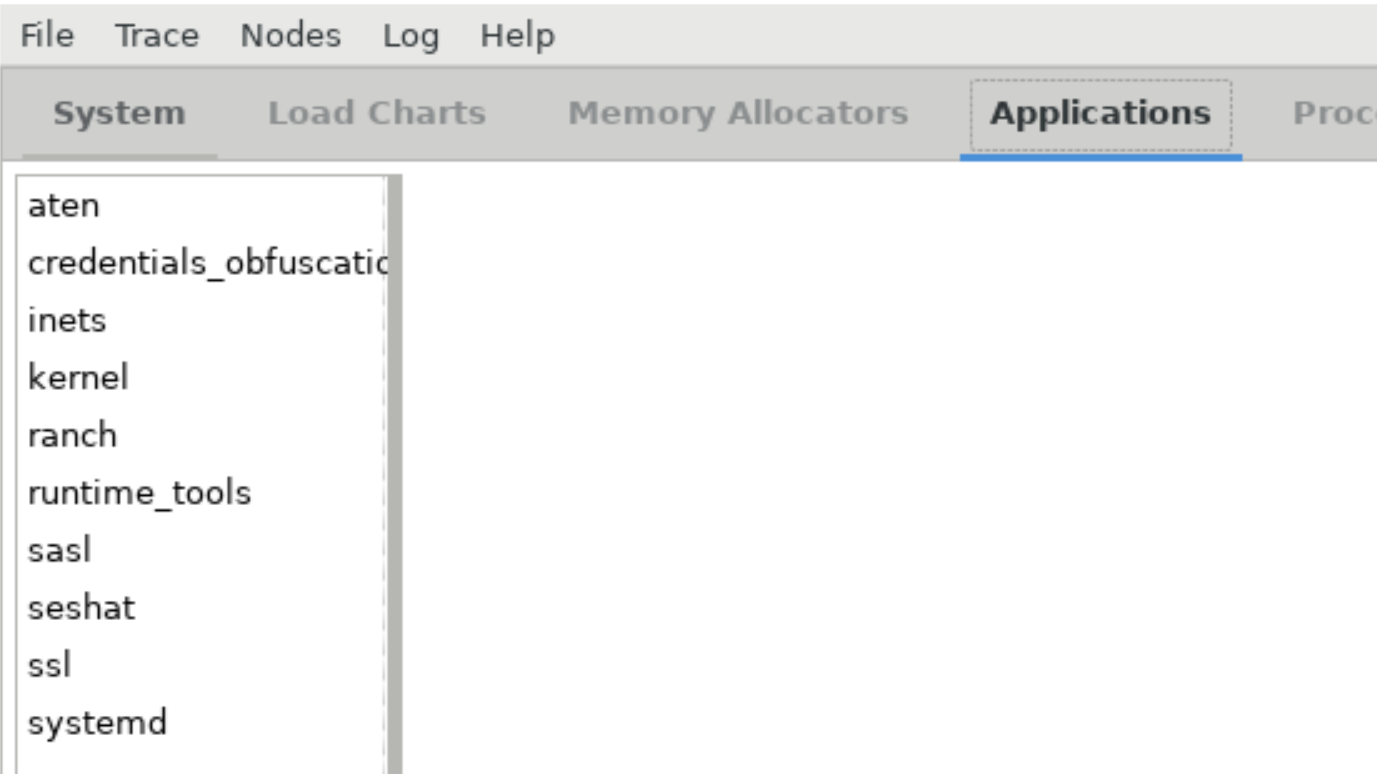
\includegraphics[width=0.85\textwidth]{image24}
\caption{RabbitMQ 停止}
\end{figure}

\subsubsection{再次开启}

\begin{lstlisting}
(rabbit@centos7-mq1)4> rabbit:start().
ok
\end{lstlisting}

\subsection{节点位置无关性}

\begin{figure}[H]
\centering
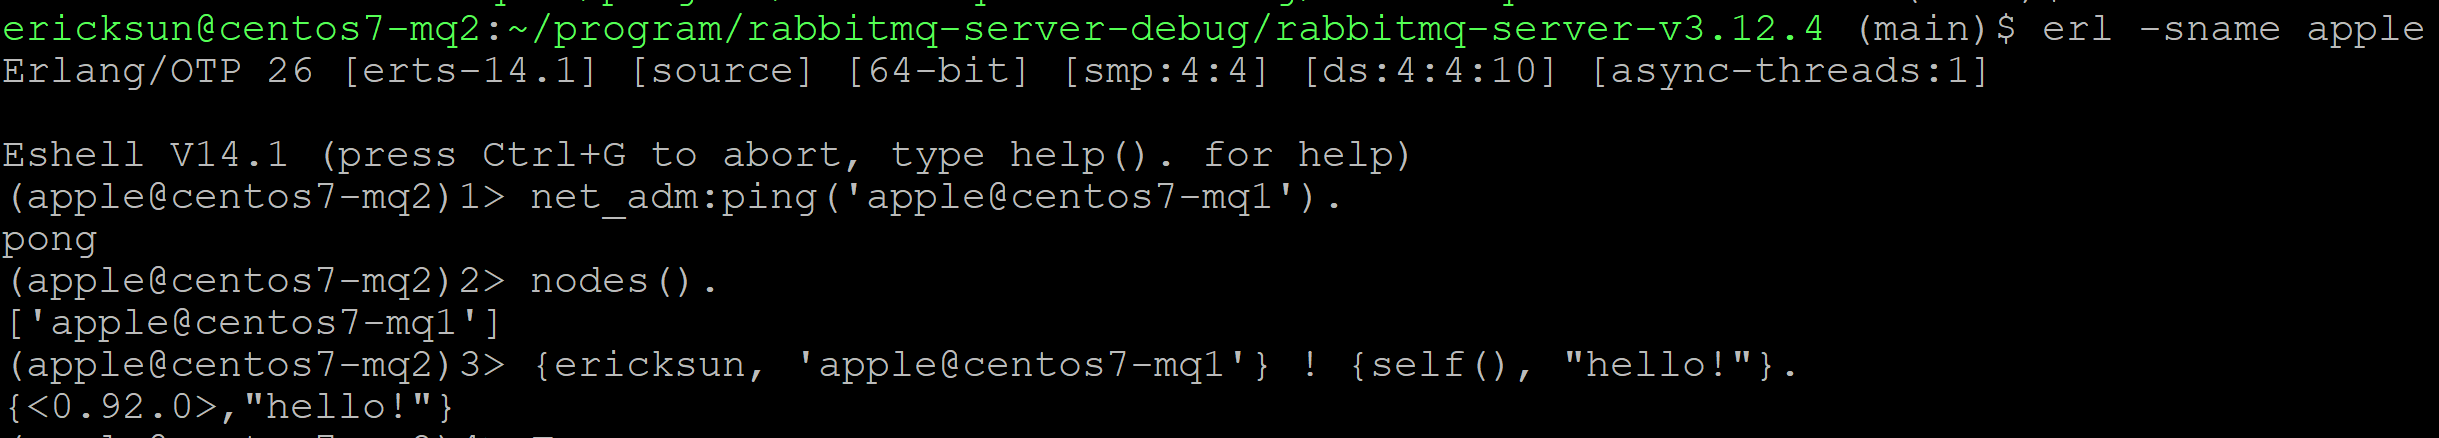
\includegraphics[width=0.85\textwidth]{image25}
\caption{节点位置无关性 (1)}
\end{figure}

\begin{figure}[H]
\centering
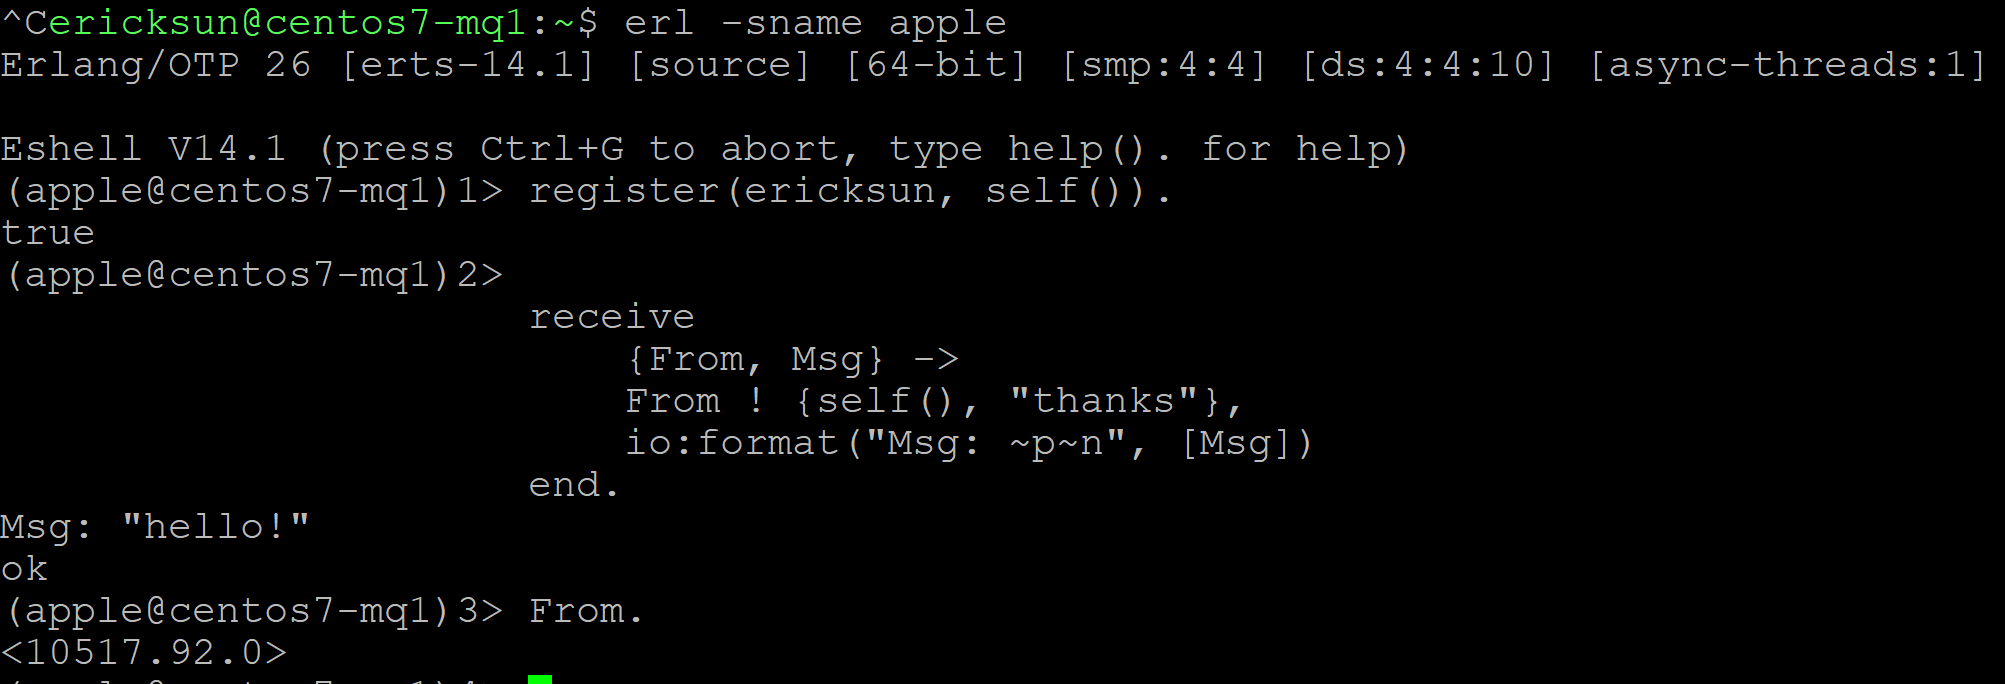
\includegraphics[width=0.85\textwidth]{image26}
\caption{节点位置无关性 (2)}
\end{figure}

\subsection{调试加载系统库和当前目录}

\subsection{列出已加载的库（符号表）}

\begin{lstlisting}
code:all_loaded().
rp(code:all_loaded()).
\end{lstlisting}

\begin{figure}[H]
\centering
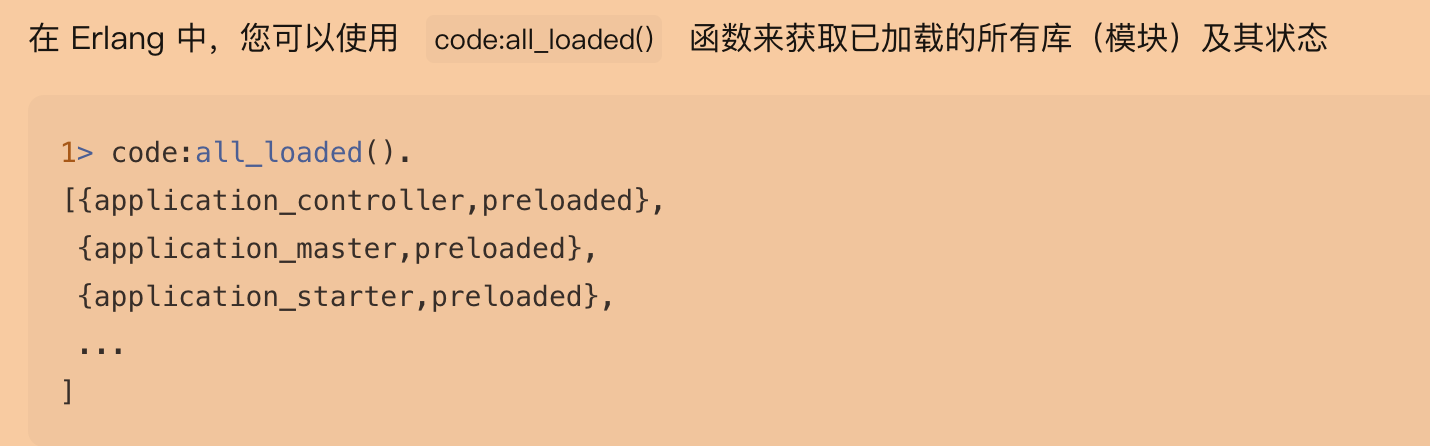
\includegraphics[width=0.85\textwidth]{image27}
\caption{已加载模块列表}
\end{figure}

\begin{itemize}[leftmargin=1.5em]
    \item 加载模块：\lstinline|l(ping).|
    \item 显示模块：\lstinline|{ping, "/home/ericksun/.../ping.beam"}|
\end{itemize}

\subsection{查看所有的路径}

使用 \lstinline|filename| 模块。

\subsection{唤起 xterm}

\begin{lstlisting}[style=shellstyle]
sudo yum install xterm.x86_64
\end{lstlisting}

\begin{figure}[H]
\centering
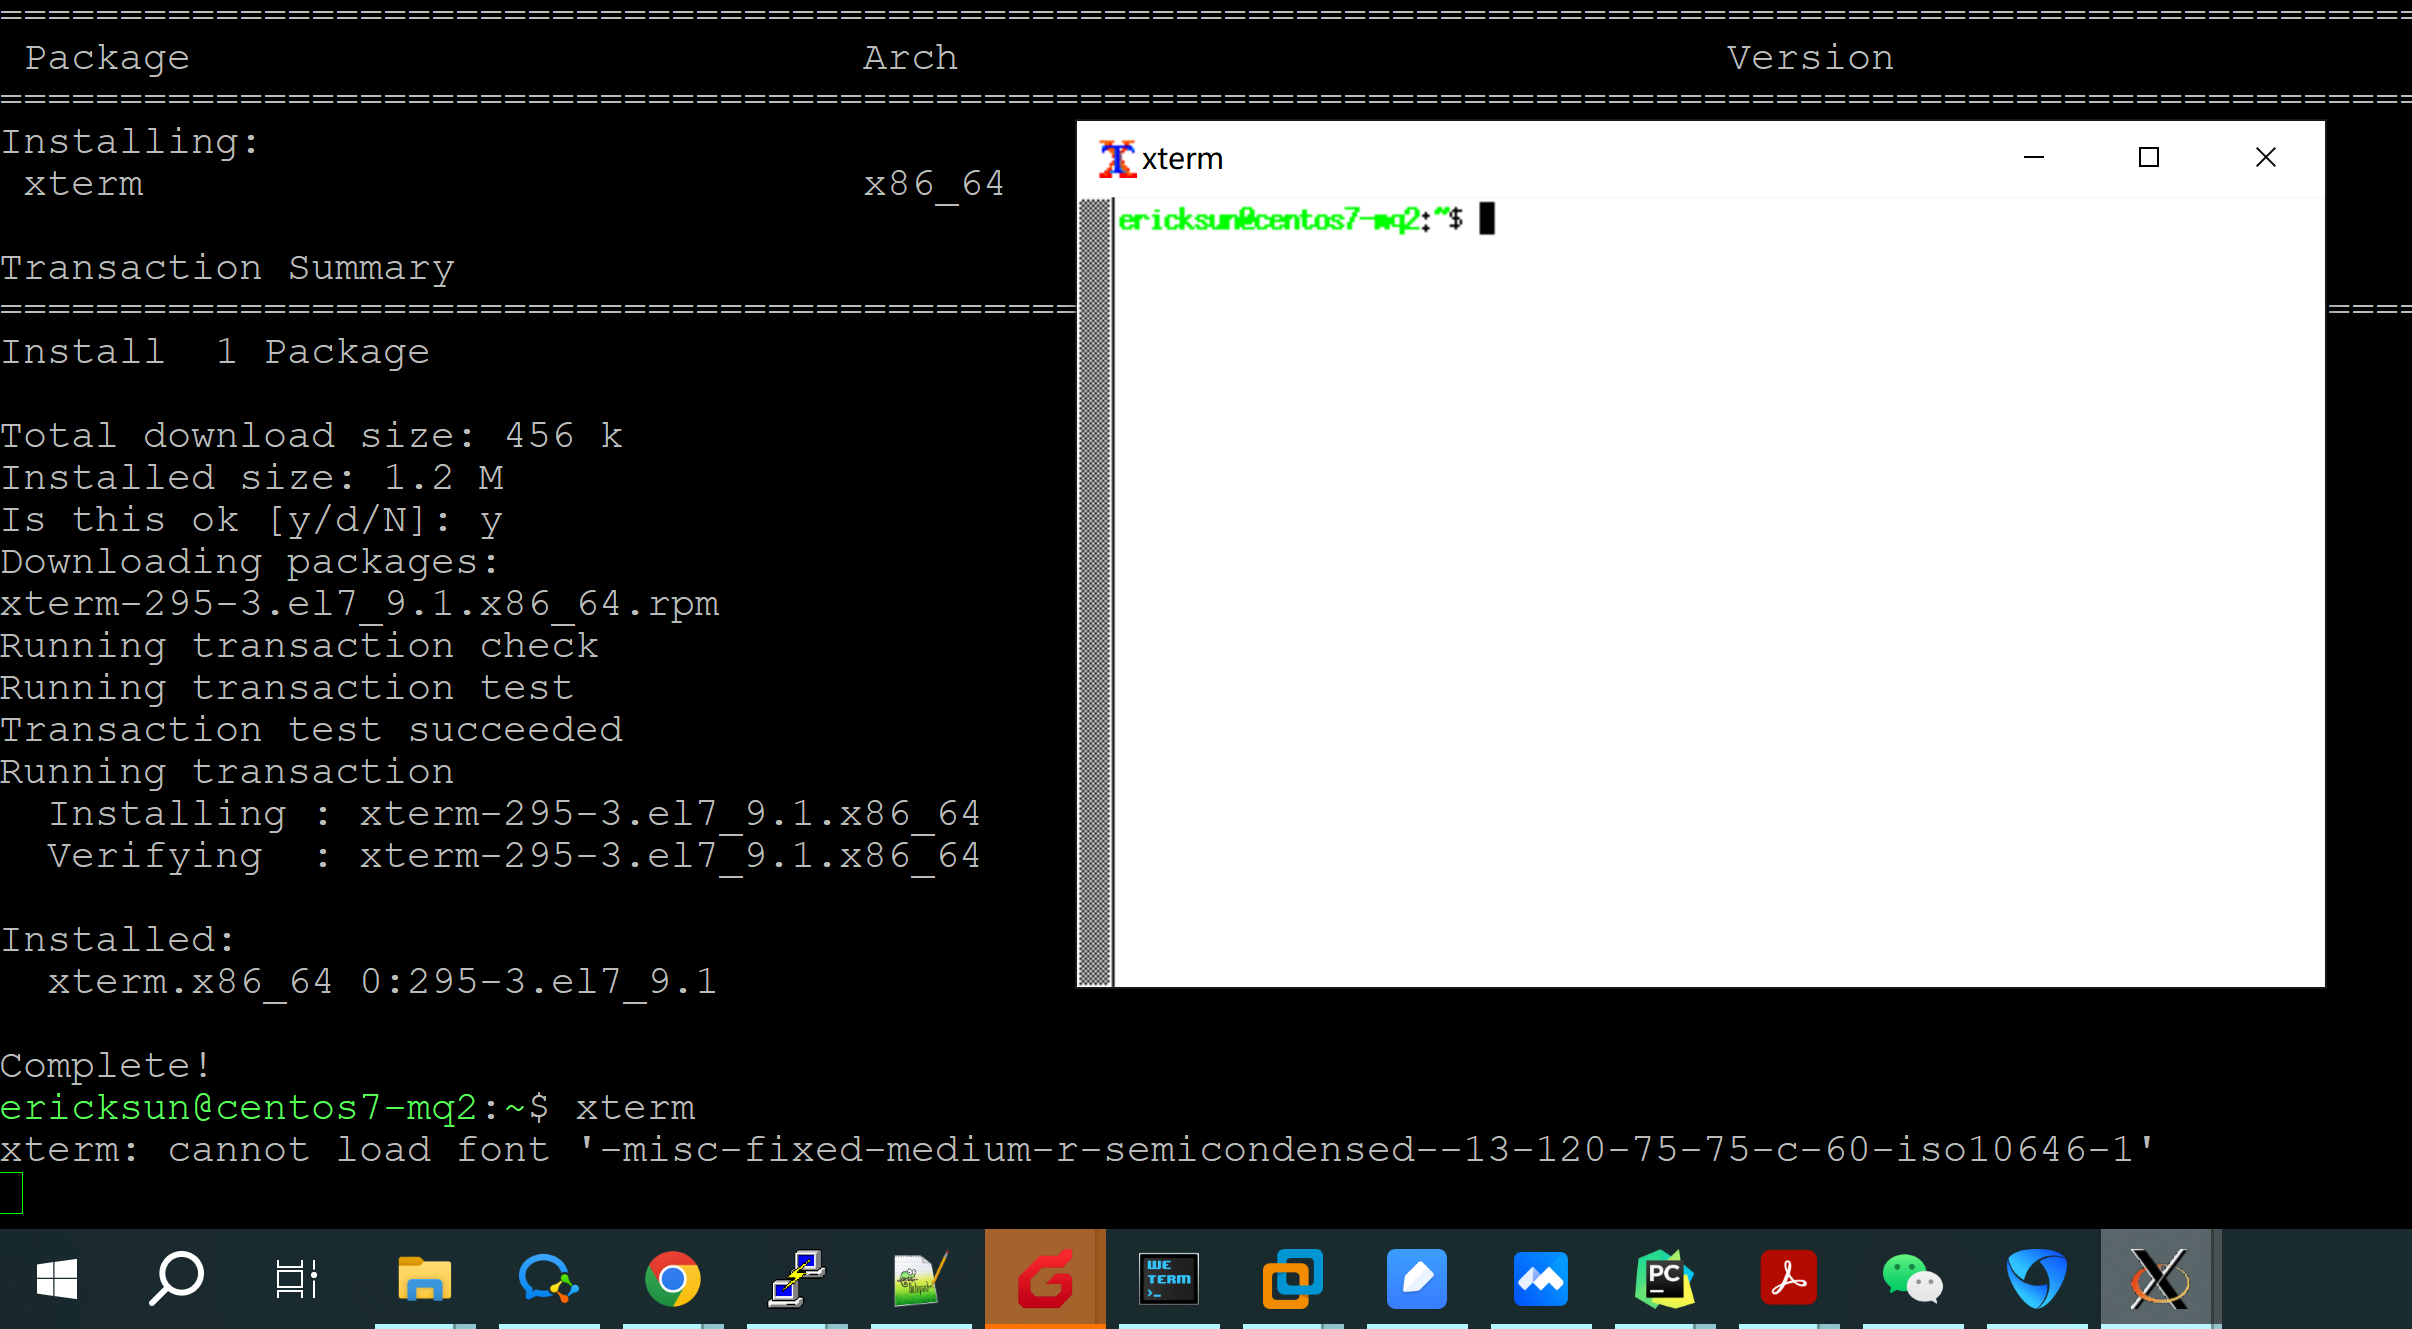
\includegraphics[width=0.85\textwidth]{image29}
\caption{xterm 界面}
\end{figure}

\subsection{查看 Monitor/Link 进程}

\begin{itemize}[leftmargin=1.5em]
    \item 查看 monitor 或 link 进程的情况
    \item 获取没有被 link 和 monitor 的进程
    \item 查看占用内存最大的进程
\end{itemize}

\subsection{日志}

\begin{itemize}[leftmargin=1.5em]
    \item \href{https://www.erlang.org/doc/man/logger.html#macros}{Erlang -- logger}
    \item \href{https://www.erlang.org/doc/man/erlang#type-reference}{Erlang -- erlang reference}
\end{itemize}

\subsection{再查清楚：日志 handler 是怎么注册的}

\subsubsection{旧版 error\_logger}

在较旧的 Erlang 版本里，\lstinline|error_logger| 是主要的日志和事件管理模块。可以借助 \lstinline|gen_event:which_handlers/1| 函数来查看 \lstinline|error_logger| 事件管理器里的所有处理程序。

\subsubsection{新版 logger 模块}

从 Erlang/OTP 21.0 版本开始，引入了新的 \lstinline|logger| 模块来替代 \lstinline|error_logger|。可以通过 \lstinline|logger:get_handler_config/0| 函数查看所有已配置的处理程序。

\subsection{查看 event 中所有的 handler}

\begin{lstlisting}
% Old version
gen_event:which_handlers(error_logger).

% New version (OTP 21+)
logger:get_handler_config().
\end{lstlisting}

% ============================================================
% Section 5: Code Management
% ============================================================
\section{代码管理}

\subsection{如何找出包依赖}

\begin{itemize}[leftmargin=1.5em]
    \item 直接启动试试：\lstinline|application:ensure_all_started(systemd).|
    \item 从 \lstinline|rebar.config| 中查看：\lstinline|{deps, [enough]}.|
    \item 使用命令：\lstinline|rebar3 deps|
    \item 使用命令：\lstinline|rebar3 tree|
    \item 使用命令：\lstinline|make list-deps|
\end{itemize}

\begin{figure}[H]
\centering
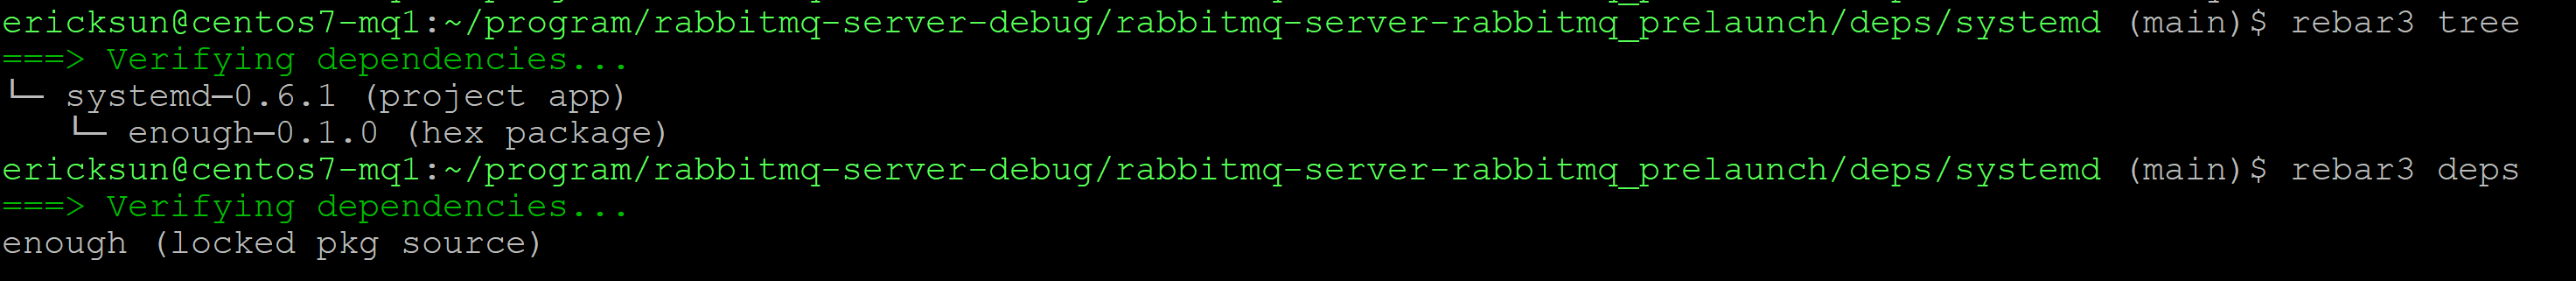
\includegraphics[width=0.85\textwidth]{image28}
\caption{rebar3 tree 输出}
\end{figure}

\subsection{如何在 rebar3 工程下设置 application 参数}

使用 \lstinline|config/sys.config| 文件设置 \lstinline|kernel| 等应用的参数。

\subsection{RabbitMQ 工程中修改代码重新编译}

需要删掉整个 \lstinline|ebin| 目录，删掉里面的内容，以及删掉 \lstinline|_build| 都没有用。

\subsection{ez Erlang --- RabbitMQ 的编译方式}

\begin{lstlisting}[style=shellstyle]
make dist DIST_AS_EZS=true
\end{lstlisting}

\subsection{Erlang 批量载入 beam 文件}

\subsection{带有头文件的编译}

参考：\href{https://stackoverflow.com/questions/74700492/erl-make-using-header-file}{Stack Overflow - erl make using header file}

\subsection{Erlang 升级（热代码加载）}

参考：\href{https://medium.com/@kansi/hot-code-loading-with-erlang-and-rebar3-8252af16605b}{Hot Code Loading with Erlang and Rebar3}

\subsection{Loading of Code From Archive Files}

\begin{itemize}[leftmargin=1.5em]
    \item \href{https://www.erlang.org/doc/man/code.html#loading-of-code-from-archive-files}{Erlang -- code}
    \item \href{https://learnyousomeerlang.com/release-is-the-word}{Learn You Some Erlang - Release is the Word}
    \item \href{https://www.erlang.org/doc/man/reltool.html}{Erlang -- reltool}
\end{itemize}

% ============================================================
% Section 6: Exception Handling
% ============================================================
\section{异常处理}

\begin{figure}[H]
\centering
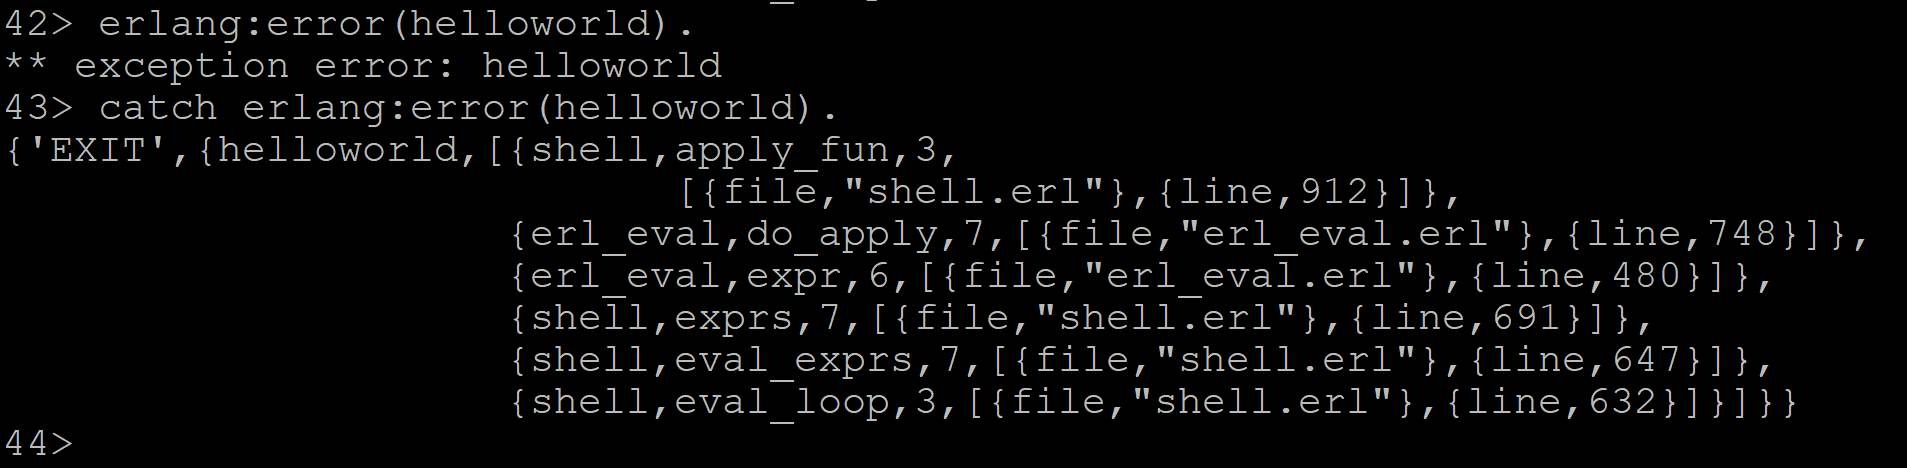
\includegraphics[width=0.85\textwidth]{image37}
\caption{异常处理机制}
\end{figure}

\begin{notebox}[catch 之后不会结束当前进程]
\end{notebox}

\begin{figure}[H]
\centering
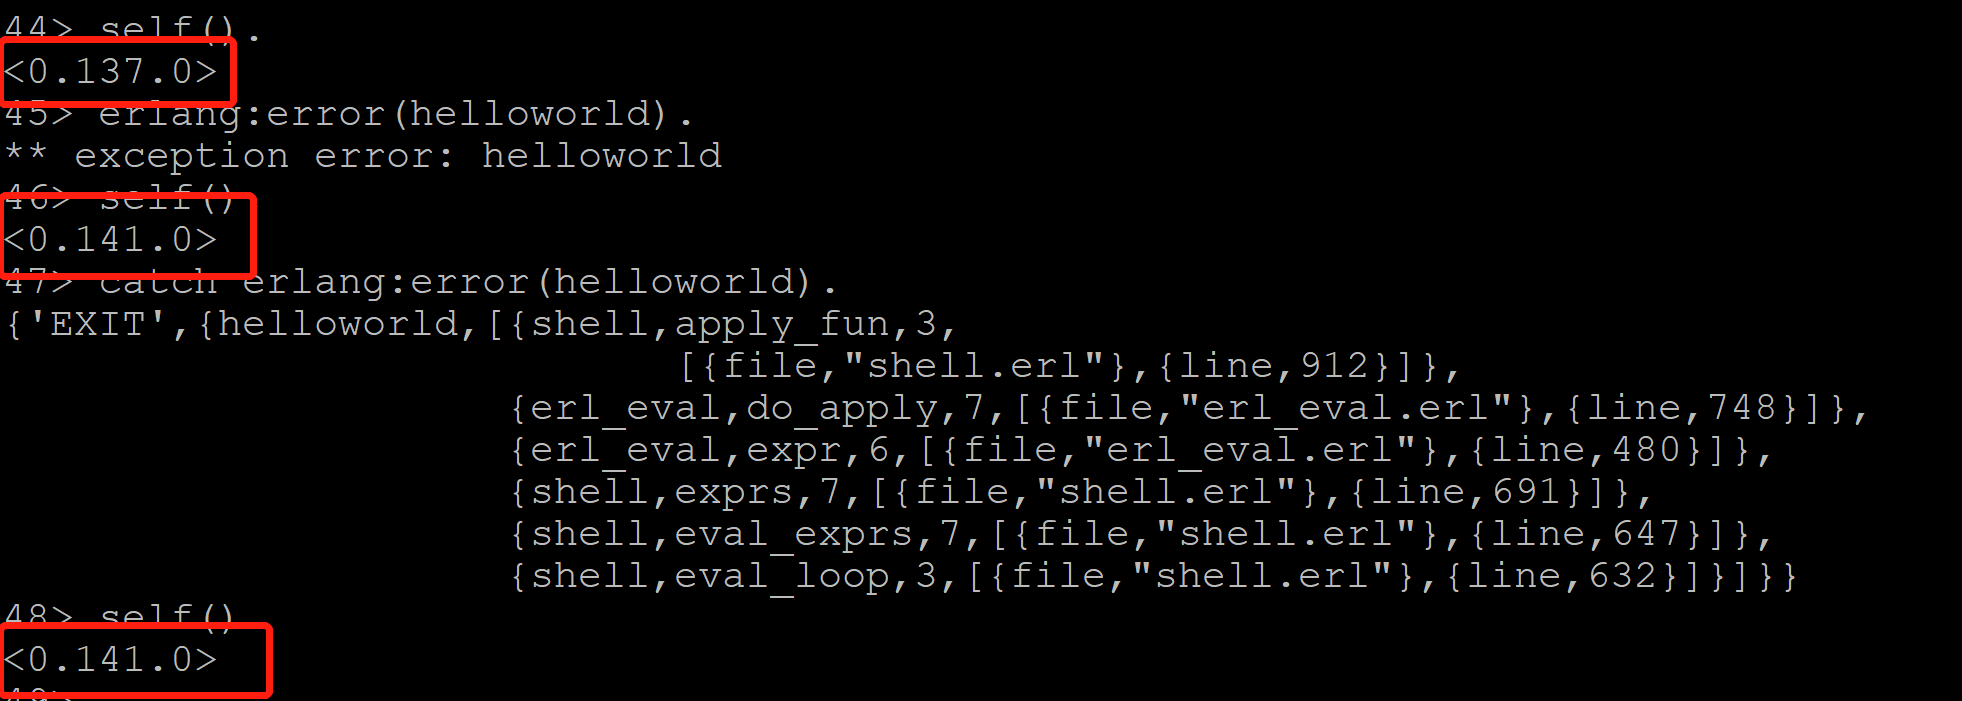
\includegraphics[width=0.85\textwidth]{image38}
\caption{catch 示例}
\end{figure}

\begin{figure}[H]
\centering
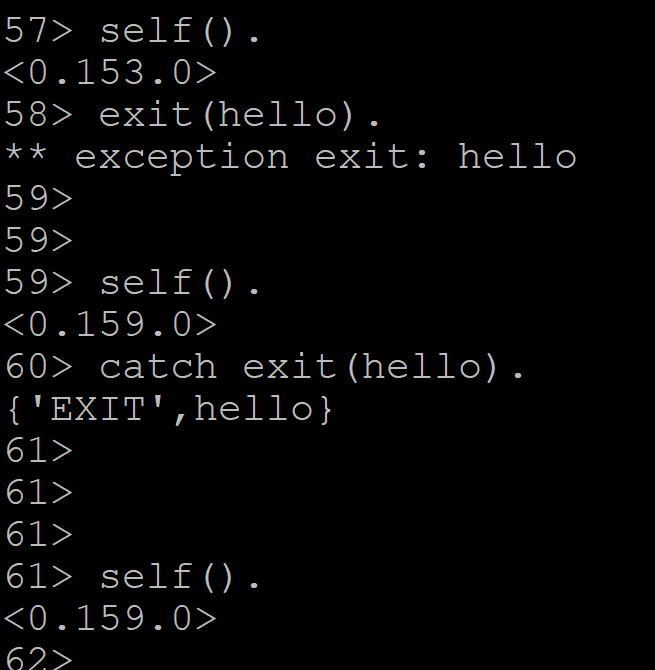
\includegraphics[width=0.35\textwidth]{image39}
\caption{异常处理示例 (1)}
\end{figure}

\begin{figure}[H]
\centering
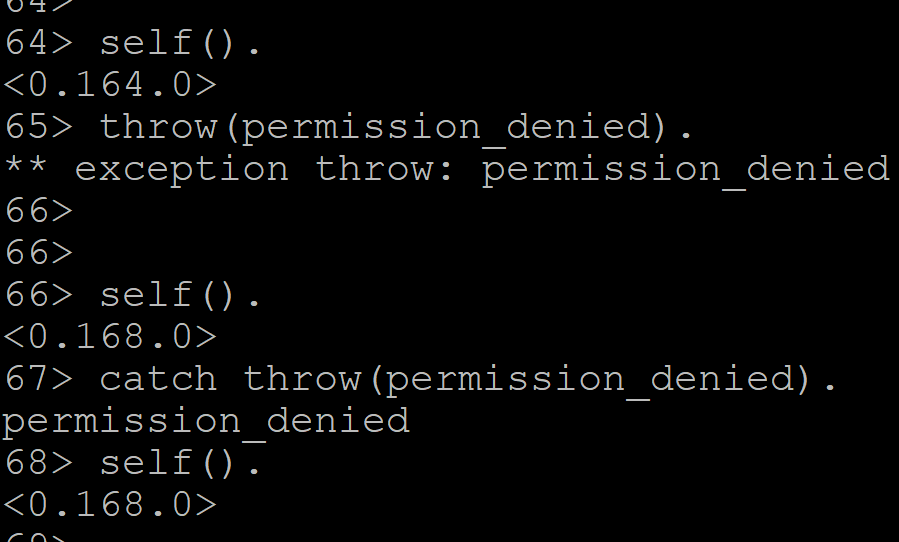
\includegraphics[width=0.6\textwidth]{image40}
\caption{异常处理示例 (2)}
\end{figure}

% ============================================================
% Section 7: Mnesia
% ============================================================
\section{Mnesia 数据库}

\subsection{定义 Record}

\begin{lstlisting}
rd(factorial, {nodeName, comment, createdOn}).
\end{lstlisting}

\subsection{加载 Record}

\begin{lstlisting}
7> rr(amqp_connection).
\end{lstlisting}

参考：\href{https://www.erlang.org/doc/man/shell}{Erlang -- shell}

\subsection{创建 Mnesia 表}

\begin{lstlisting}
rd(factorial, {nodeName, comment, createdOn}).

Result = mnesia:create_table(factorial,
    [{attributes, record_info(fields, factorial)},
     {type, bag},
     {ram_copies, [node()]}]).

Result2 = mnesia:create_table(factorial1,
    [{attributes, record_info(fields, factorial)},
     {type, bag},
     {disc_copies, [node()]}]).
\end{lstlisting}

\subsection{查看 Mnesia 表信息}

\begin{figure}[H]
\centering
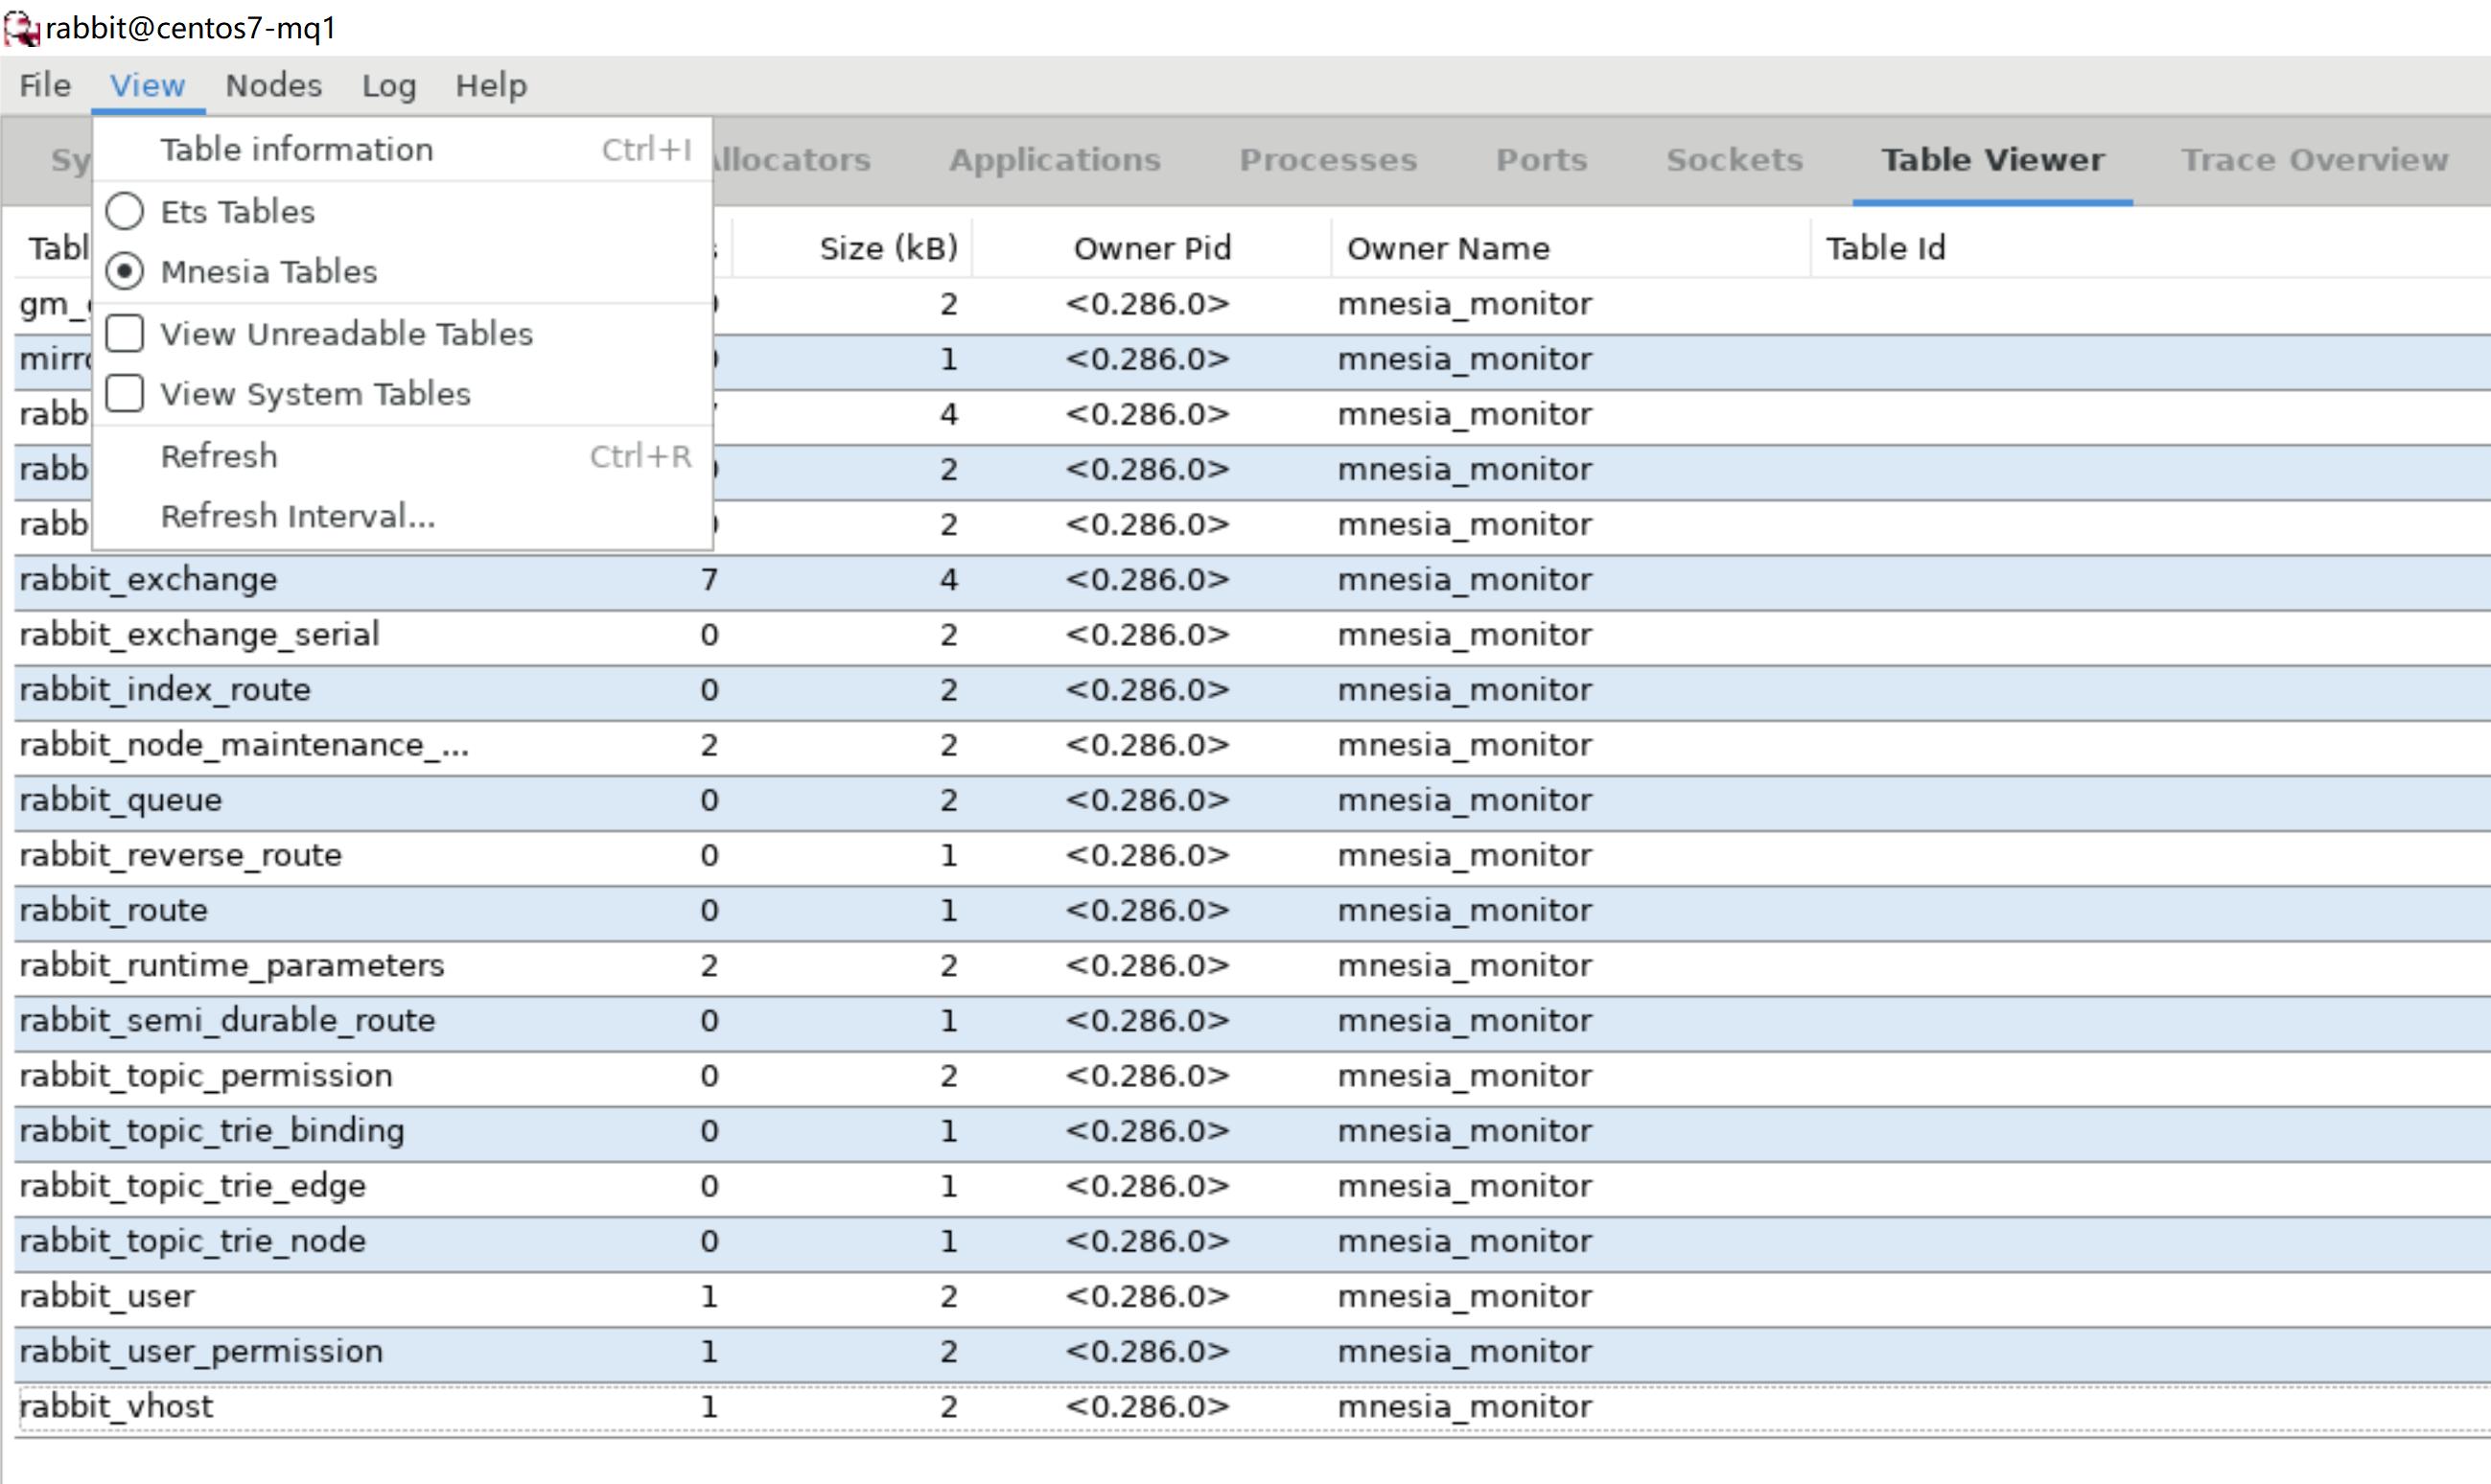
\includegraphics[width=0.85\textwidth]{image2}
\caption{Mnesia 表信息}
\end{figure}

% ============================================================
% Section 8: Process and Messaging
% ============================================================
\section{进程与消息}

\subsection{进程的注册和获取}

\begin{figure}[H]
\centering
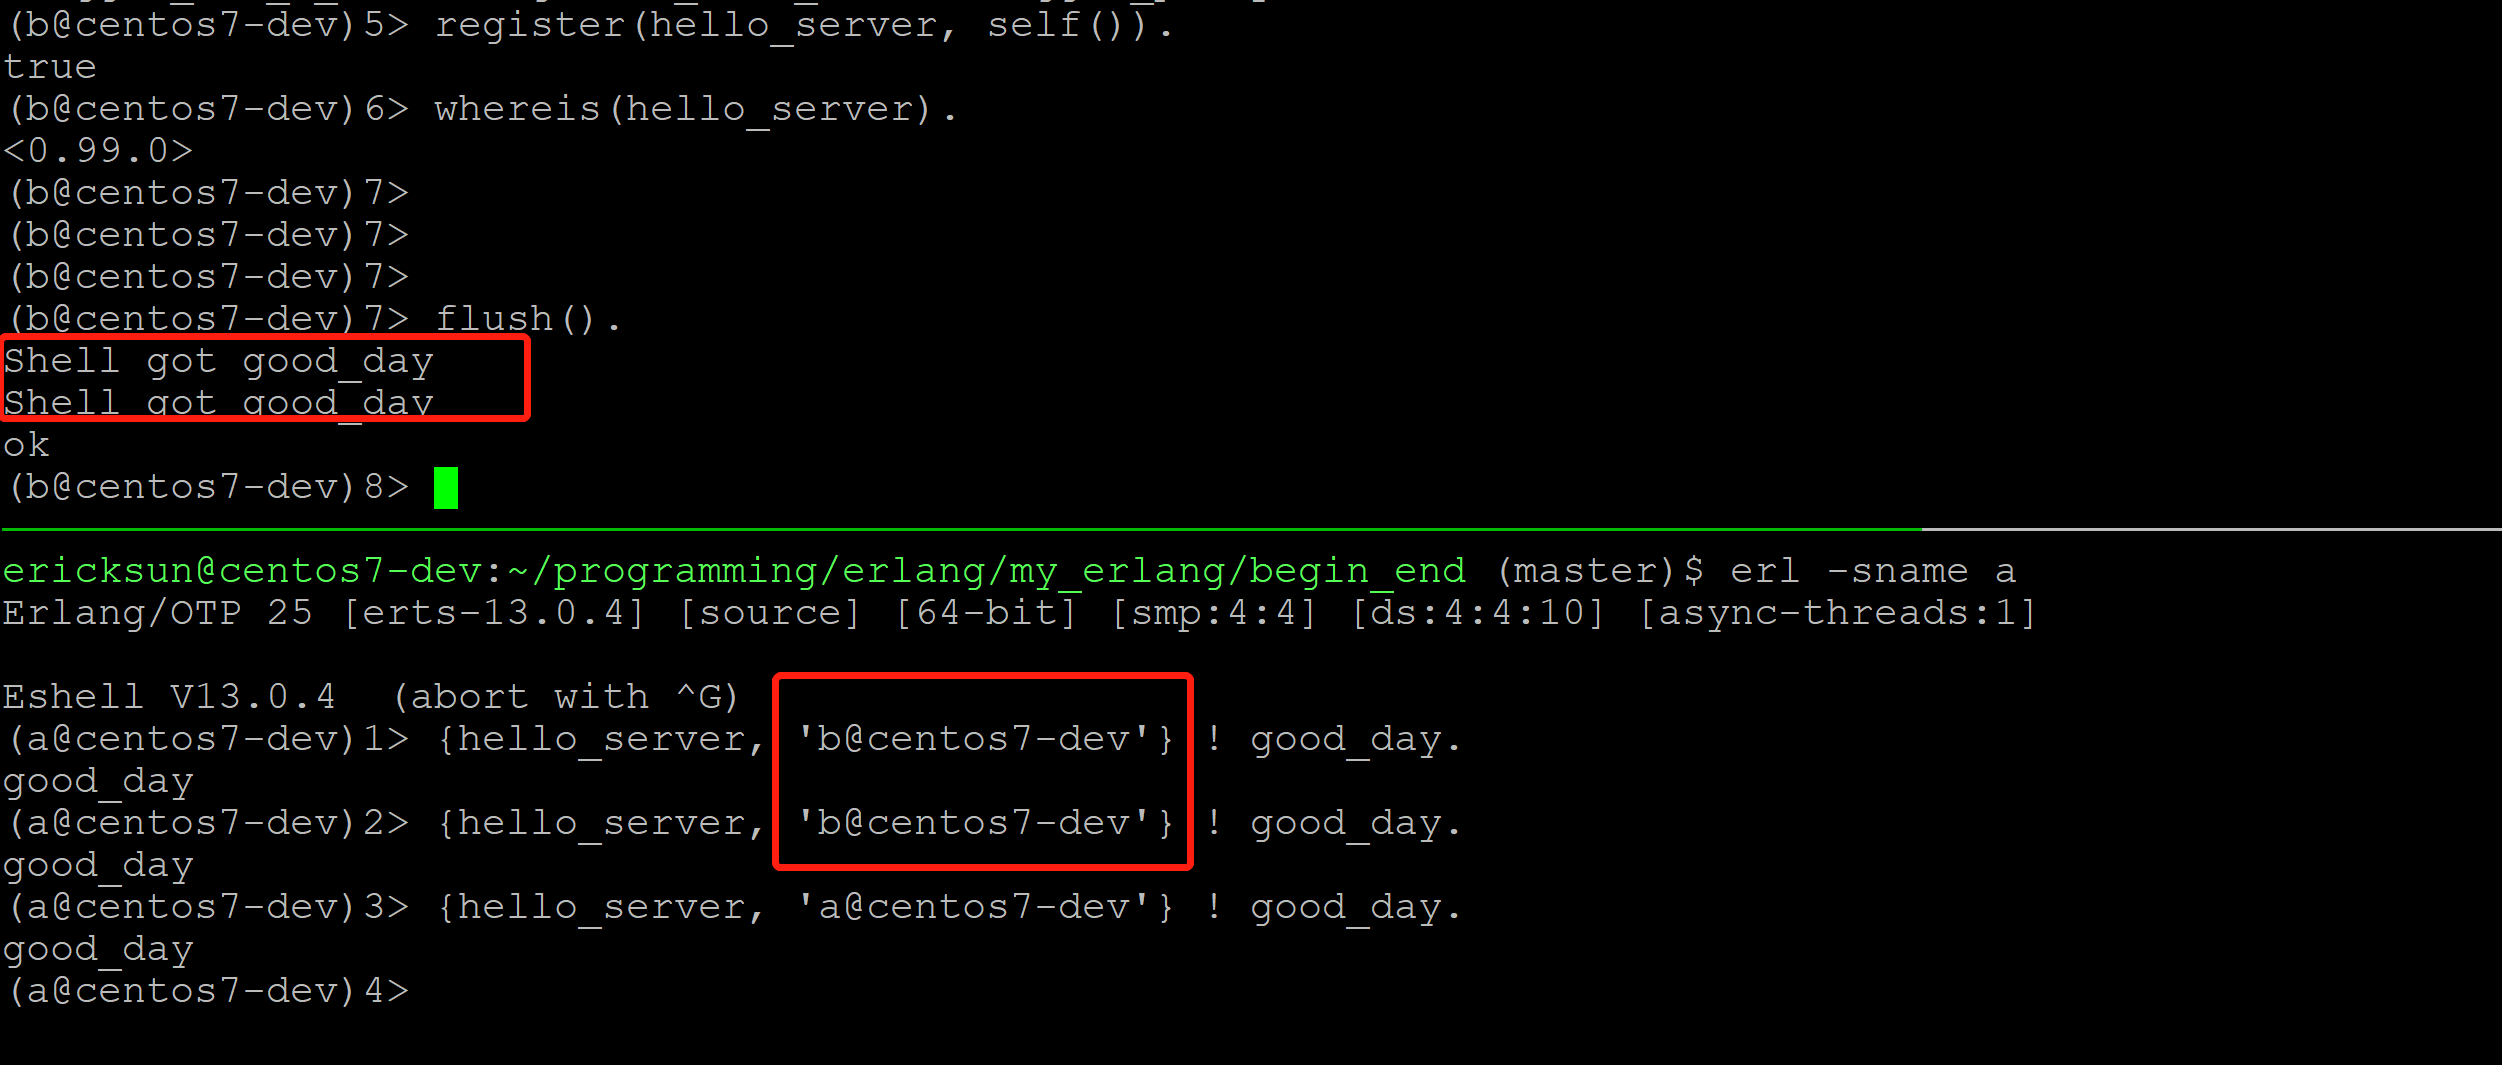
\includegraphics[width=0.85\textwidth]{image48}
\caption{进程注册与获取}
\end{figure}

\subsection{发送信息到远程节点}

向另一节点上的注册进程发送消息的格式：

\begin{lstlisting}
{pong, Pong_Node} ! {ping, self()},
\end{lstlisting}

使用 \lstinline|{registered_name, node_name}| 元组代替单独的 \lstinline|registered_name|。

\begin{figure}[H]
\centering
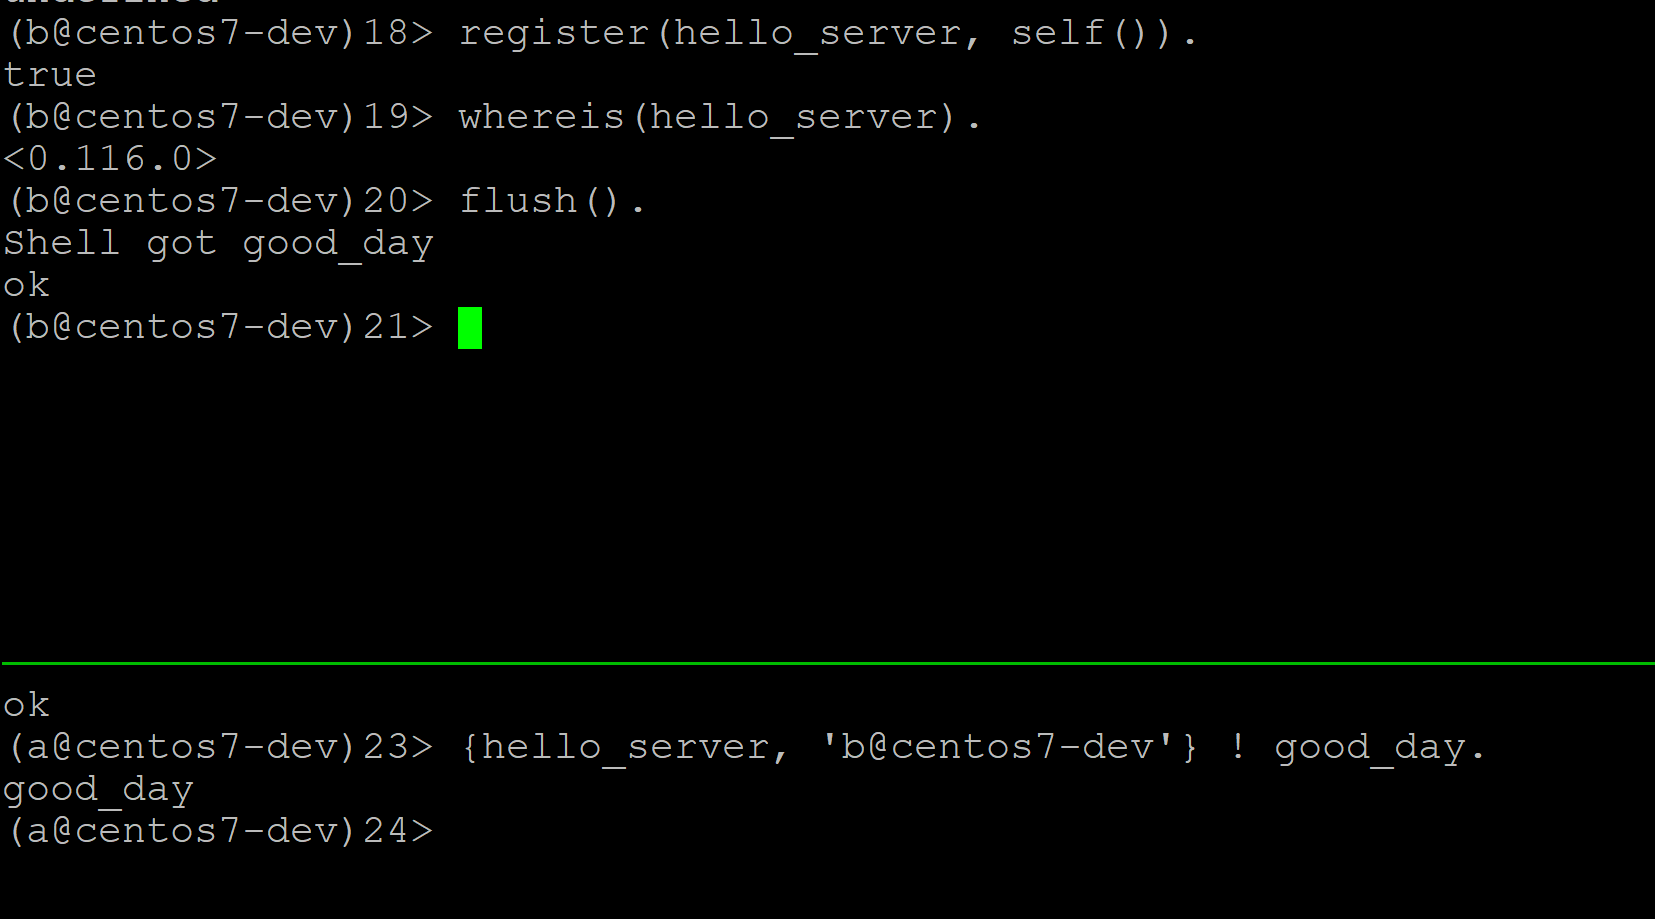
\includegraphics[width=0.85\textwidth]{image47}
\caption{远程消息发送}
\end{figure}

参考：\href{https://www.erlang.org/doc/getting_started/conc_prog.html#message-passing}{Erlang -- Concurrent Programming}

\subsection{获取远程进程 PID：通过 register}

\begin{figure}[H]
\centering
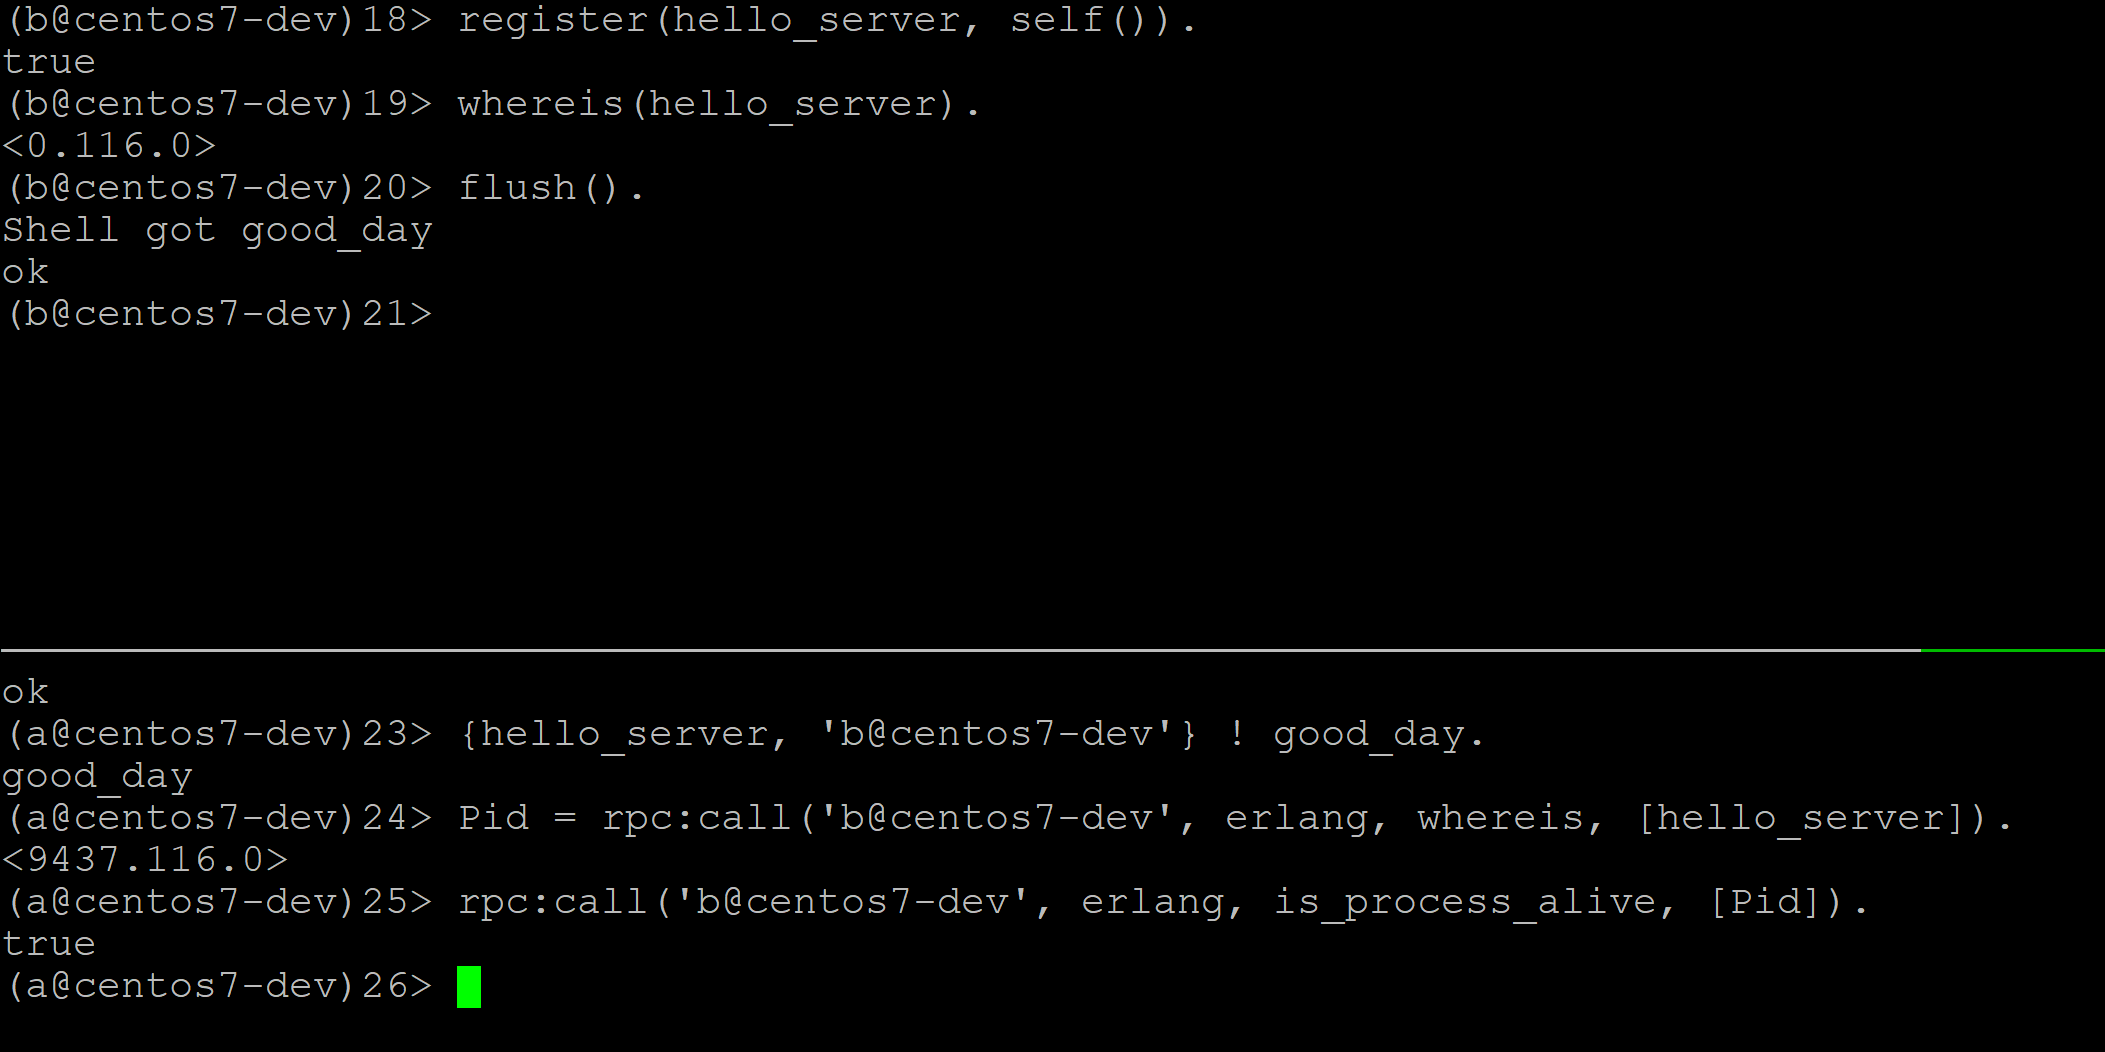
\includegraphics[width=0.85\textwidth]{image49}
\caption{通过 register 获取远程 PID (1)}
\end{figure}

\begin{figure}[H]
\centering
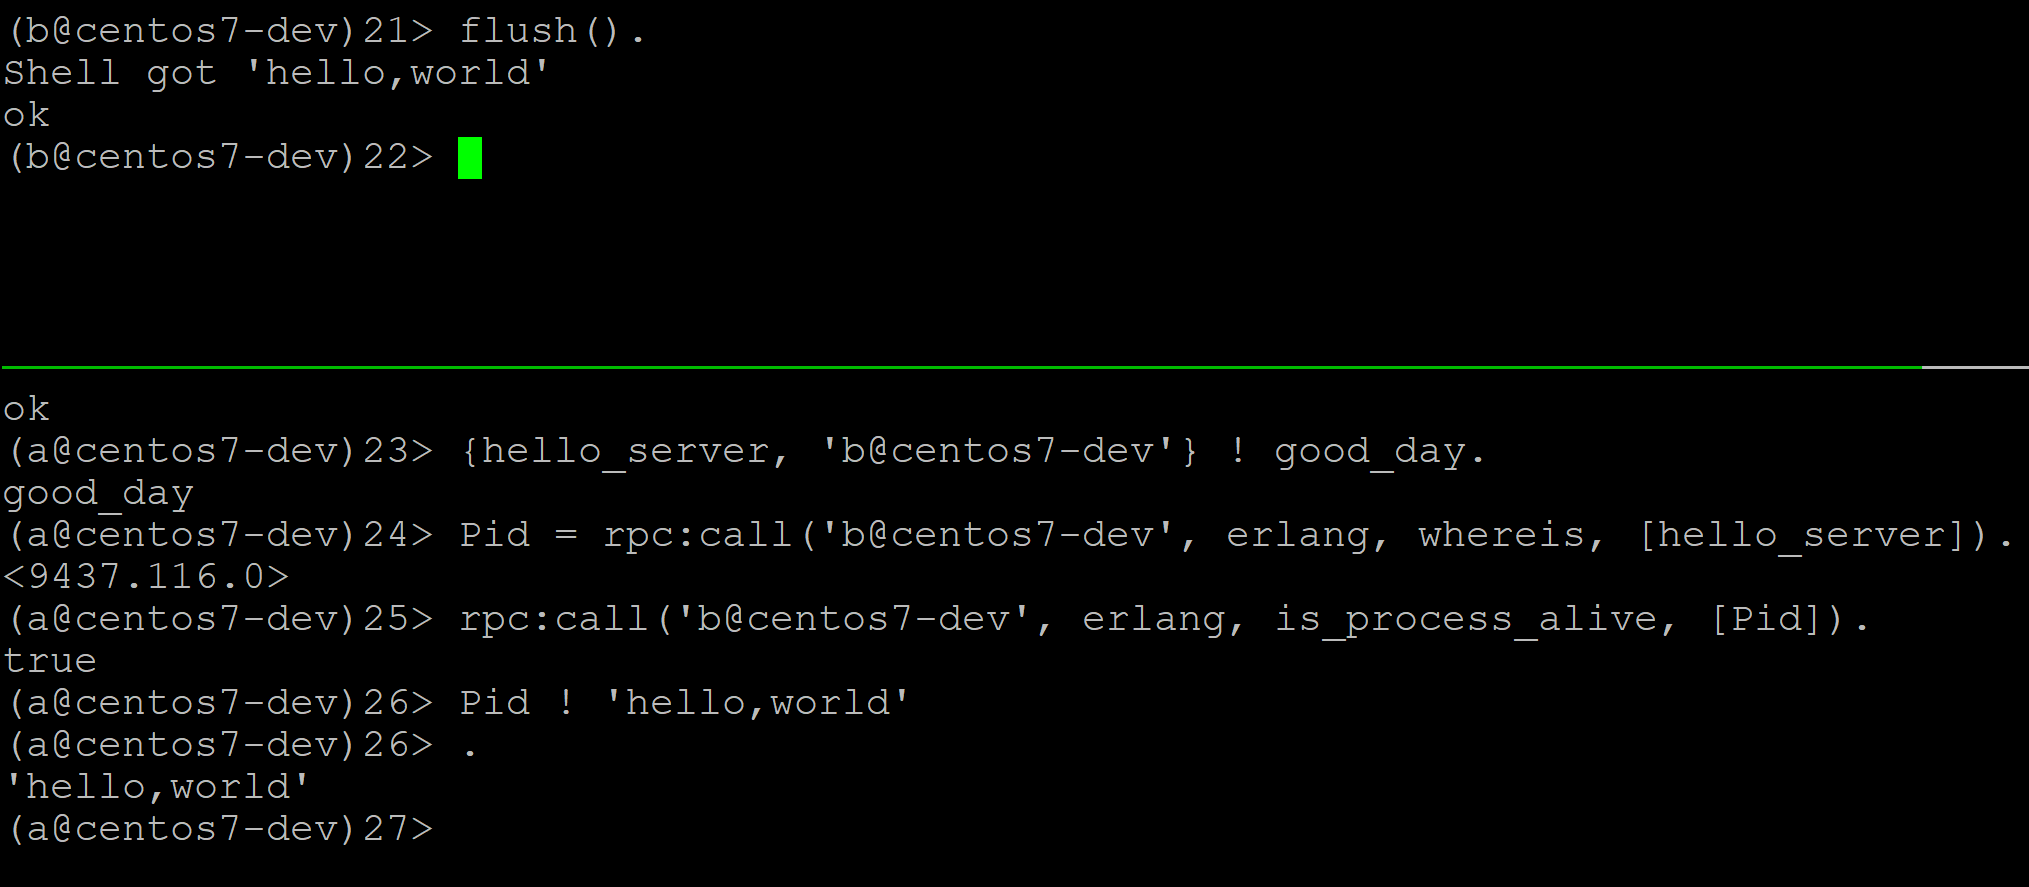
\includegraphics[width=0.85\textwidth]{image50}
\caption{通过 register 获取远程 PID (2)}
\end{figure}

\begin{figure}[H]
\centering
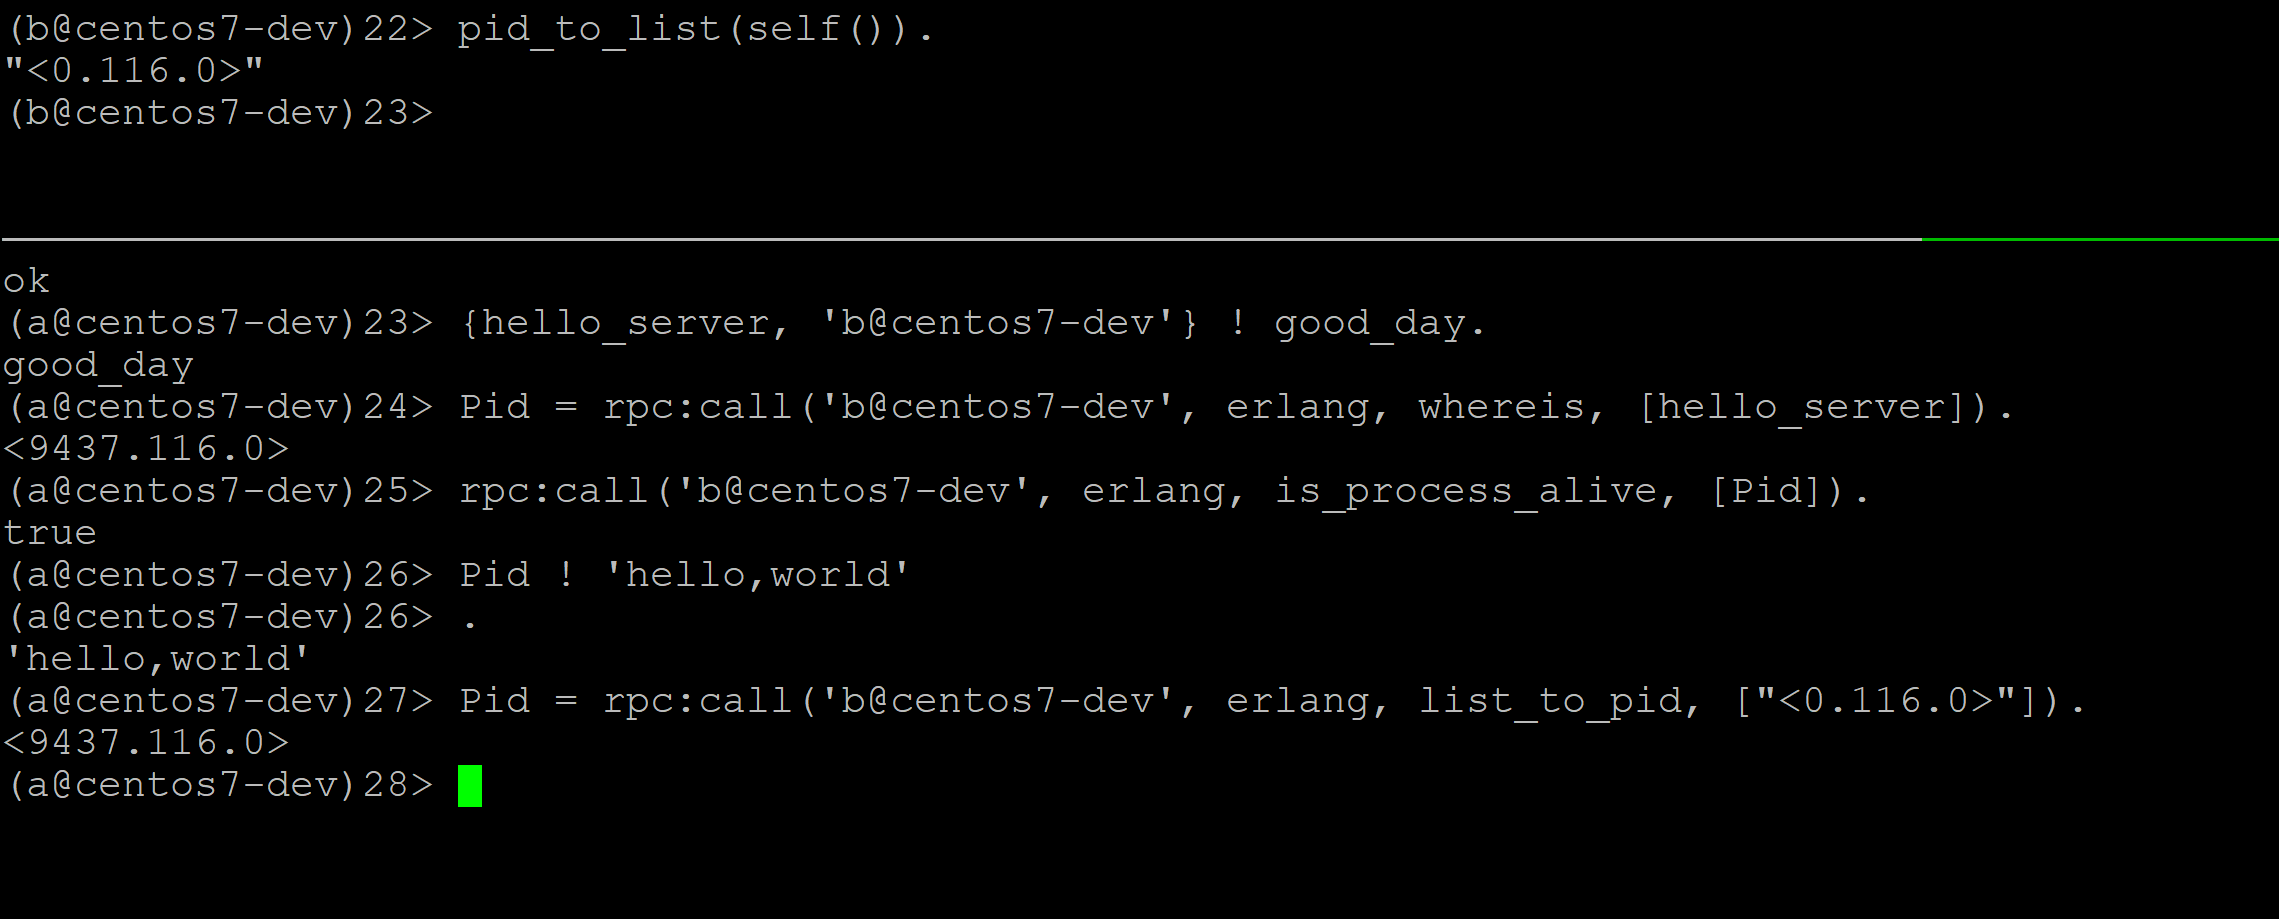
\includegraphics[width=0.85\textwidth]{image51}
\caption{通过 register 获取远程 PID (3)}
\end{figure}

\subsection{直接用远程 PID 发送消息}

\subsection{io\_request 与 group\_leader}

\begin{figure}[H]
\centering
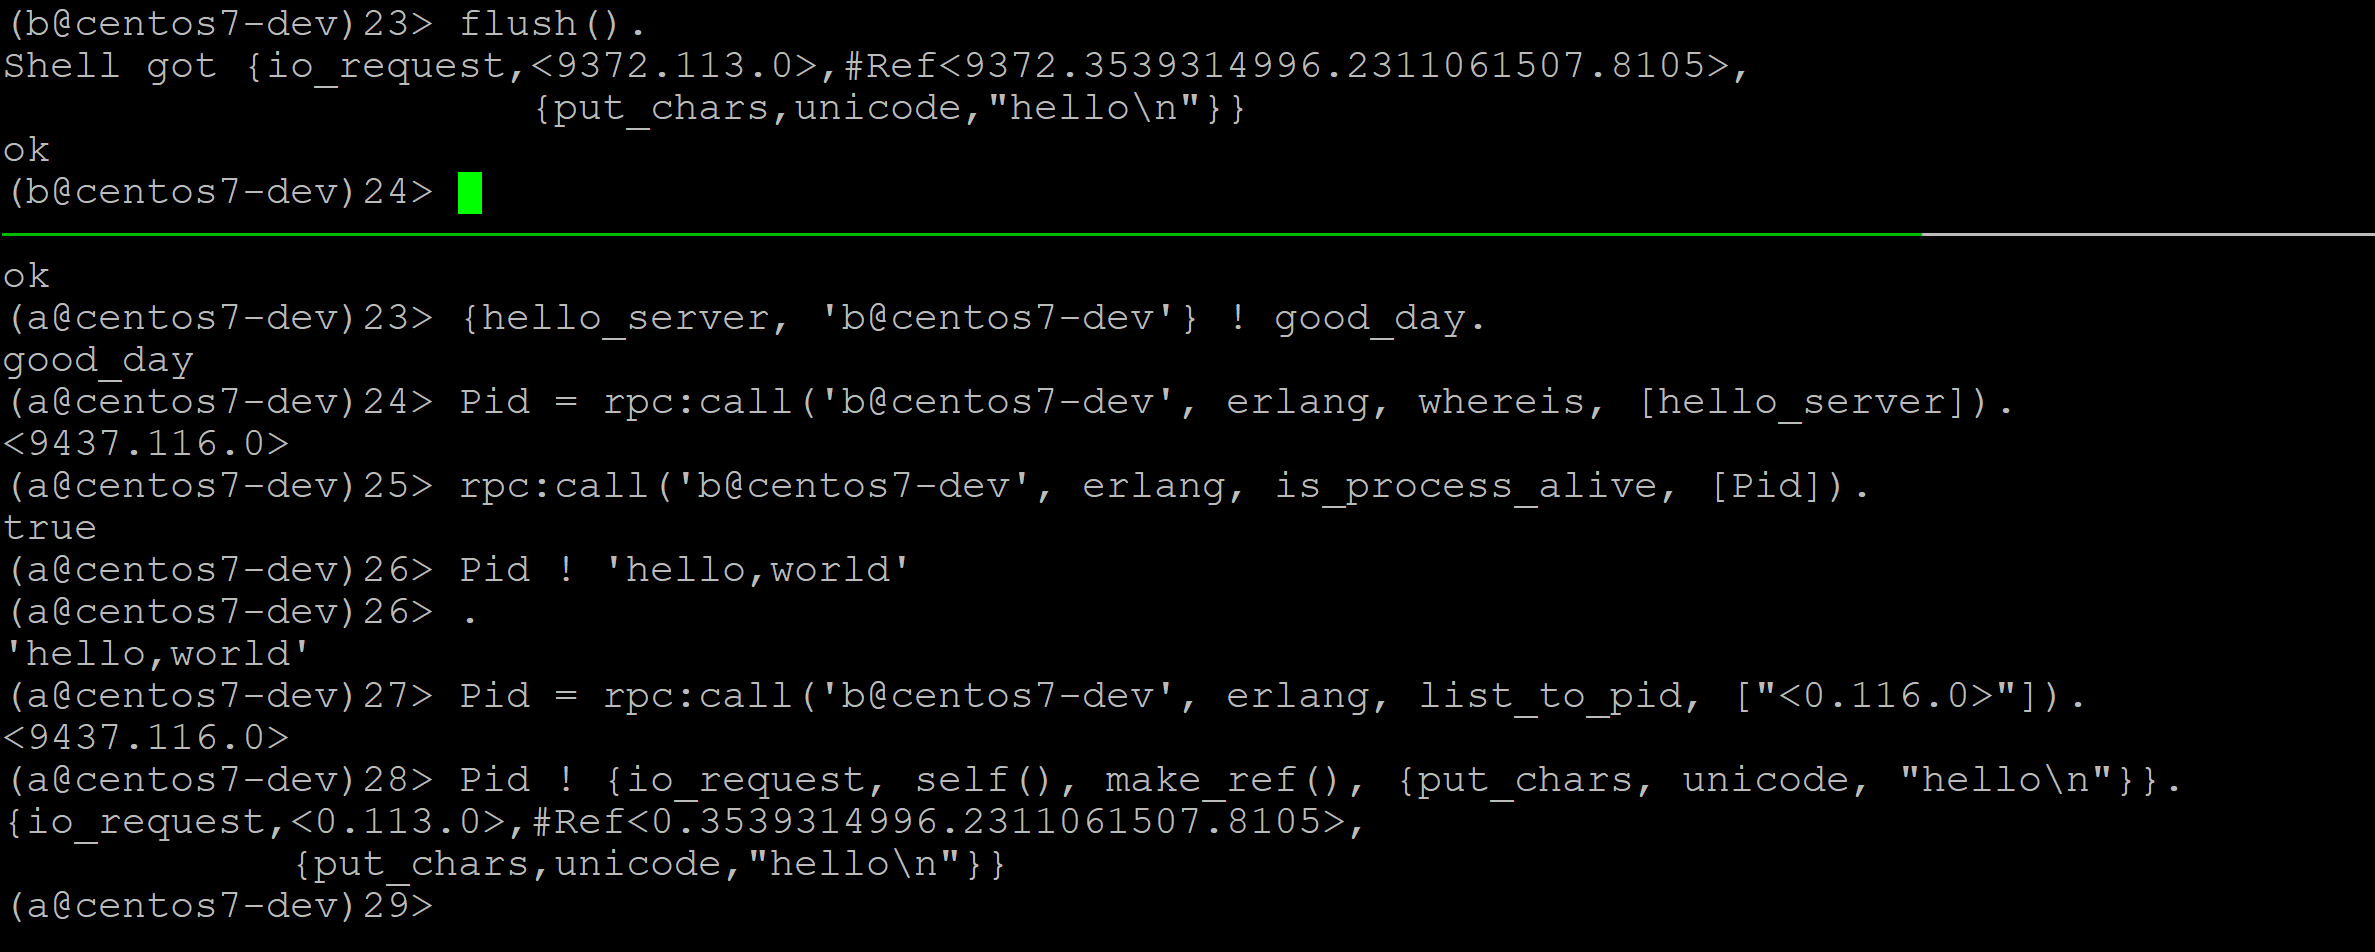
\includegraphics[width=0.85\textwidth]{image52}
\caption{io\_request 发送到远程}
\end{figure}

\lstinline|io_request| 发送到远程，无法直接执行打印的时候，放到消息队列。

\begin{figure}[H]
\centering
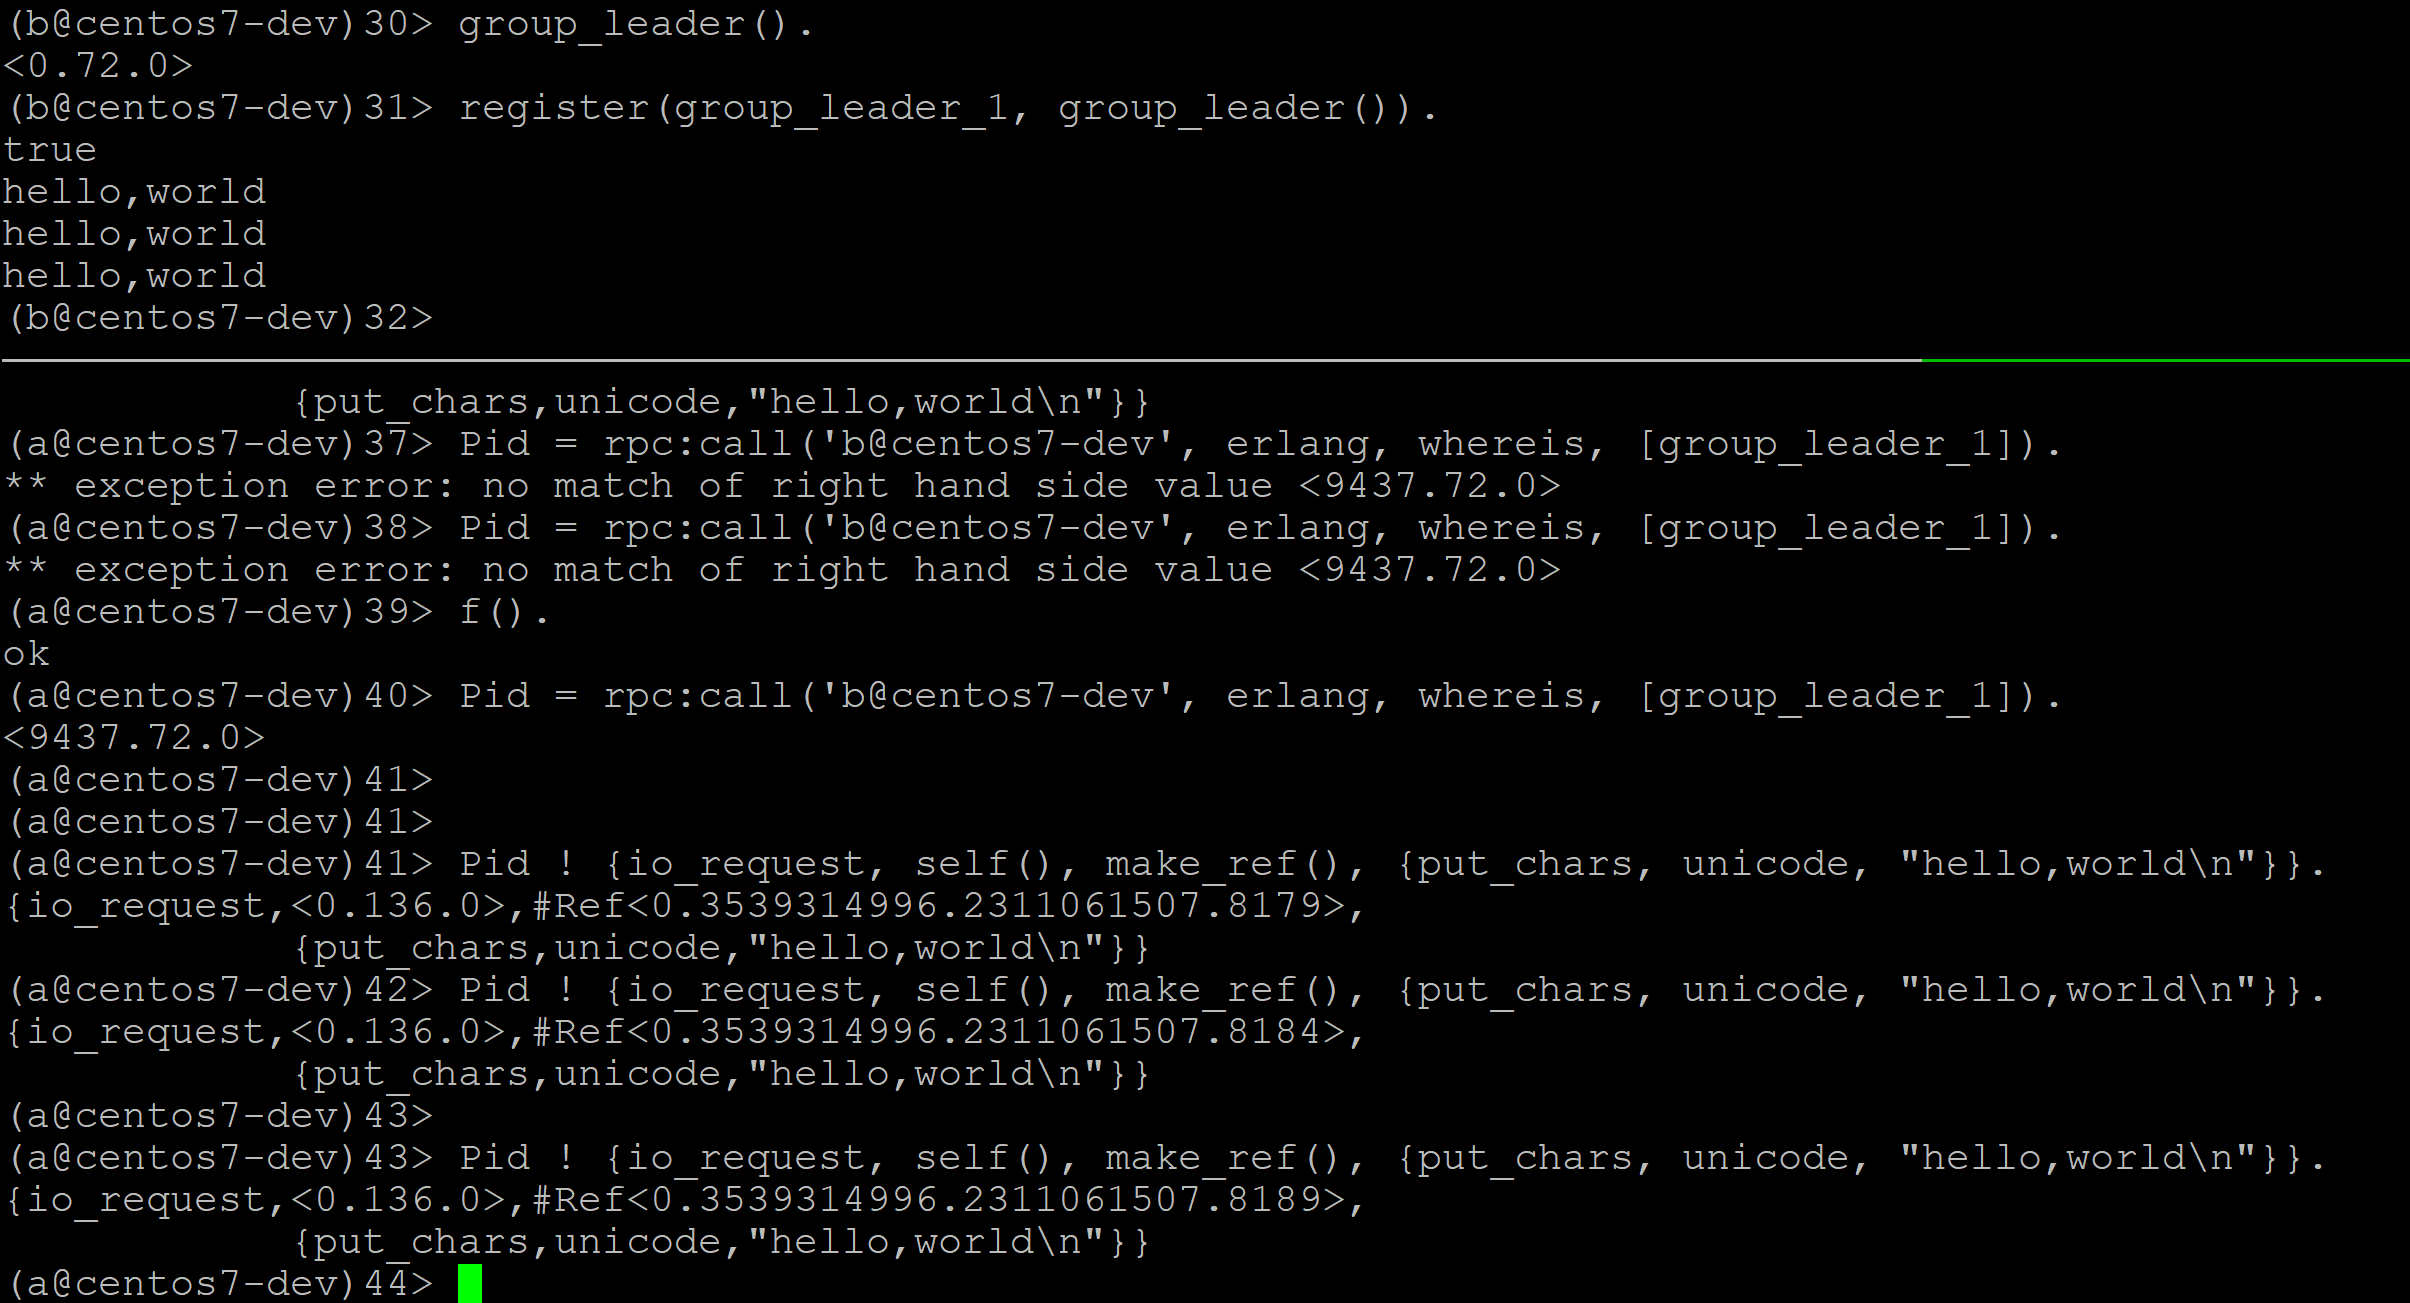
\includegraphics[width=0.85\textwidth]{image53}
\caption{发给 group\_leader 直接执行}
\end{figure}

发给 \lstinline|group_leader| 直接执行，不会放到进程的消息队列中。

\subsection{Observer 观察消息队列}

\begin{figure}[H]
\centering
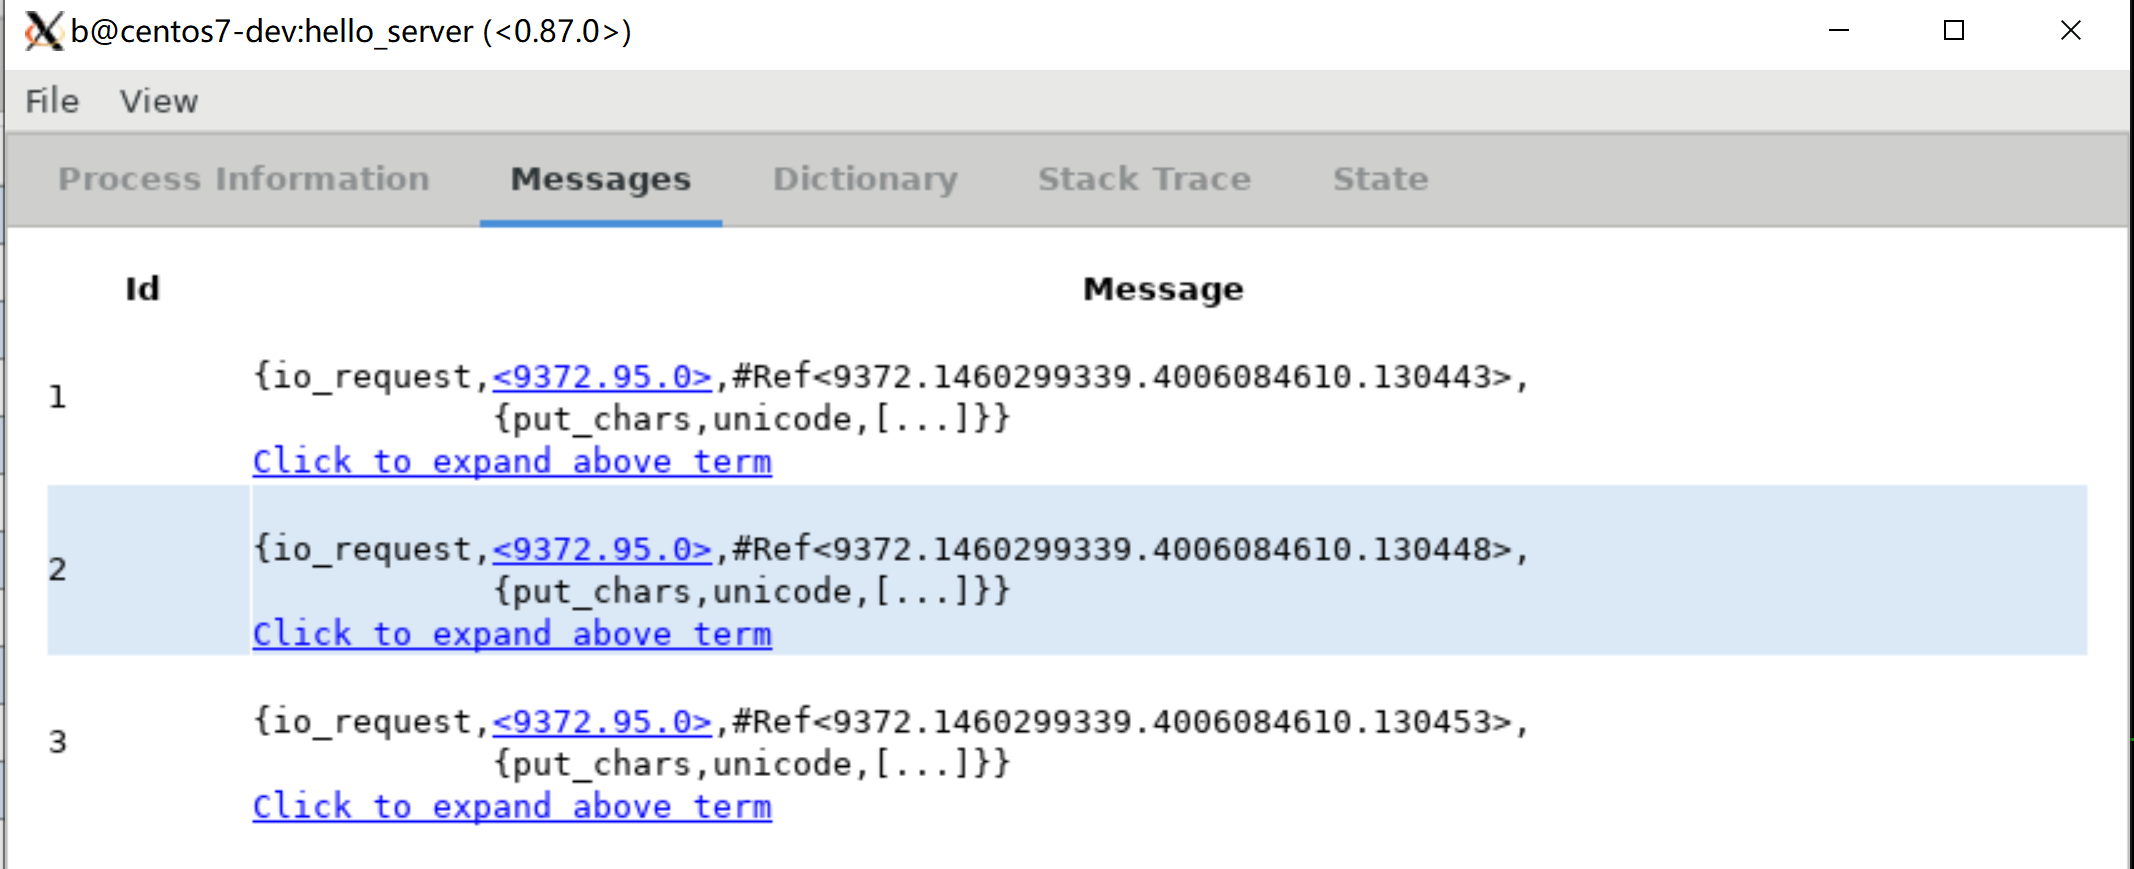
\includegraphics[width=0.85\textwidth]{image54}
\caption{Observer 消息队列 (1)}
\end{figure}

\begin{figure}[H]
\centering
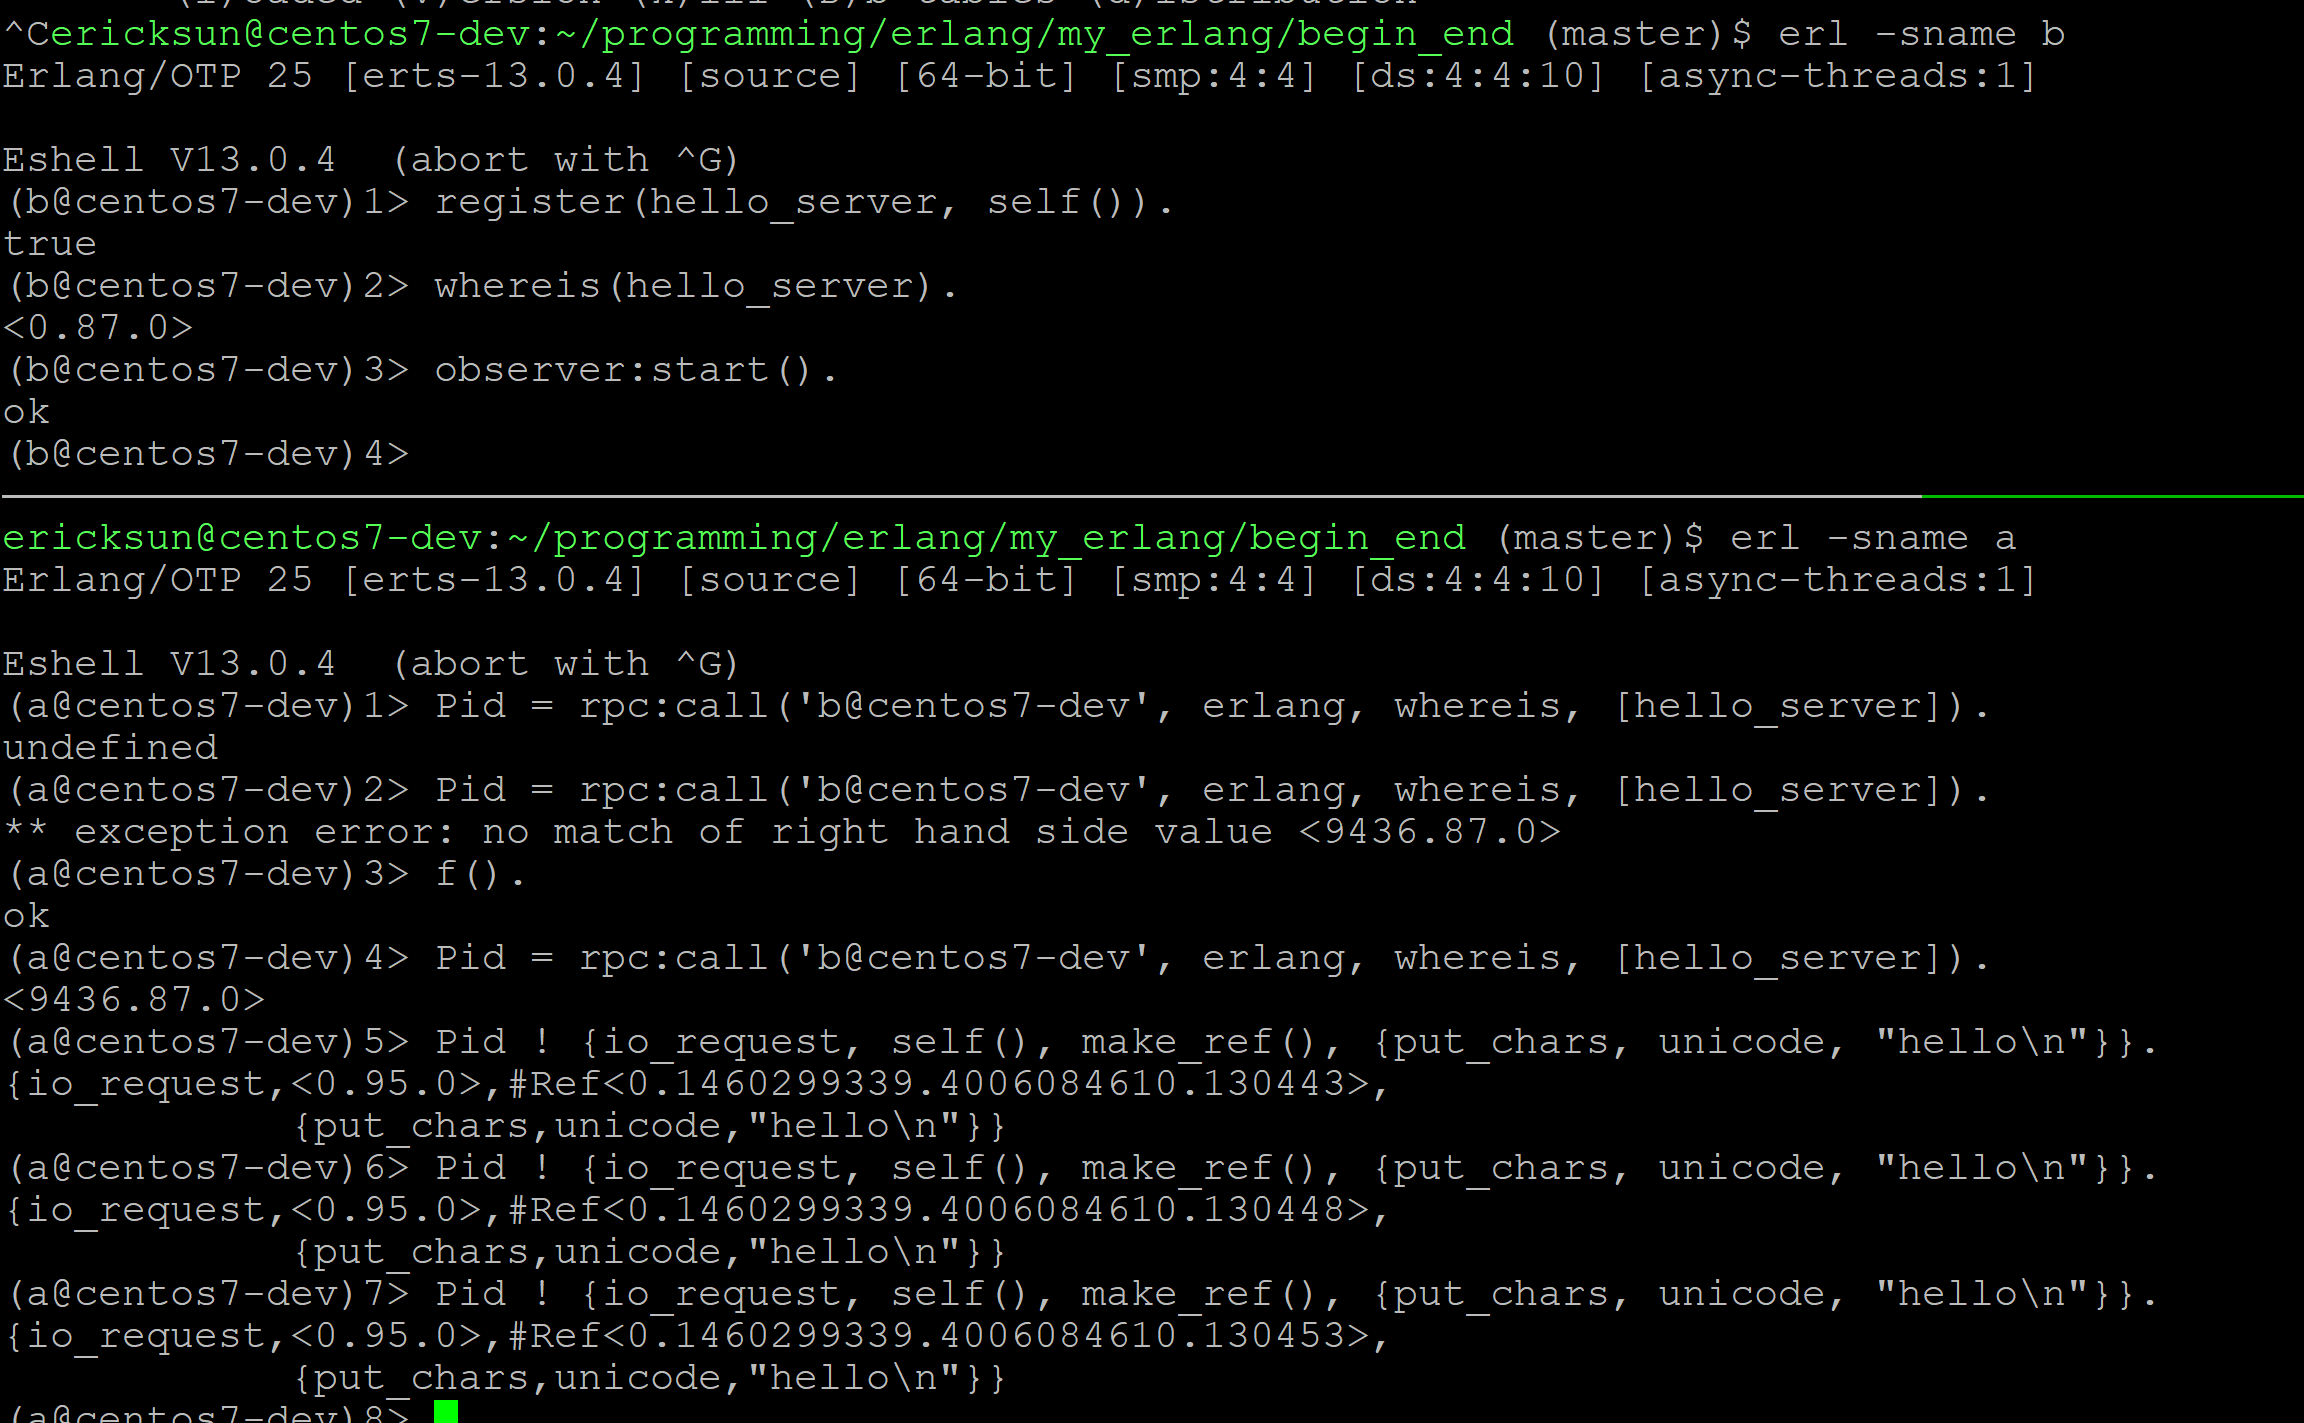
\includegraphics[width=0.85\textwidth]{image55}
\caption{Observer 消息队列 (2)}
\end{figure}

\subsection{获取进程列表与进程信息}

\begin{itemize}[leftmargin=1.5em]
    \item 获取进程列表
    \item 获取进程信息
\end{itemize}

\subsection{Erlang/OTP 并发编程实践}

\begin{figure}[H]
\centering
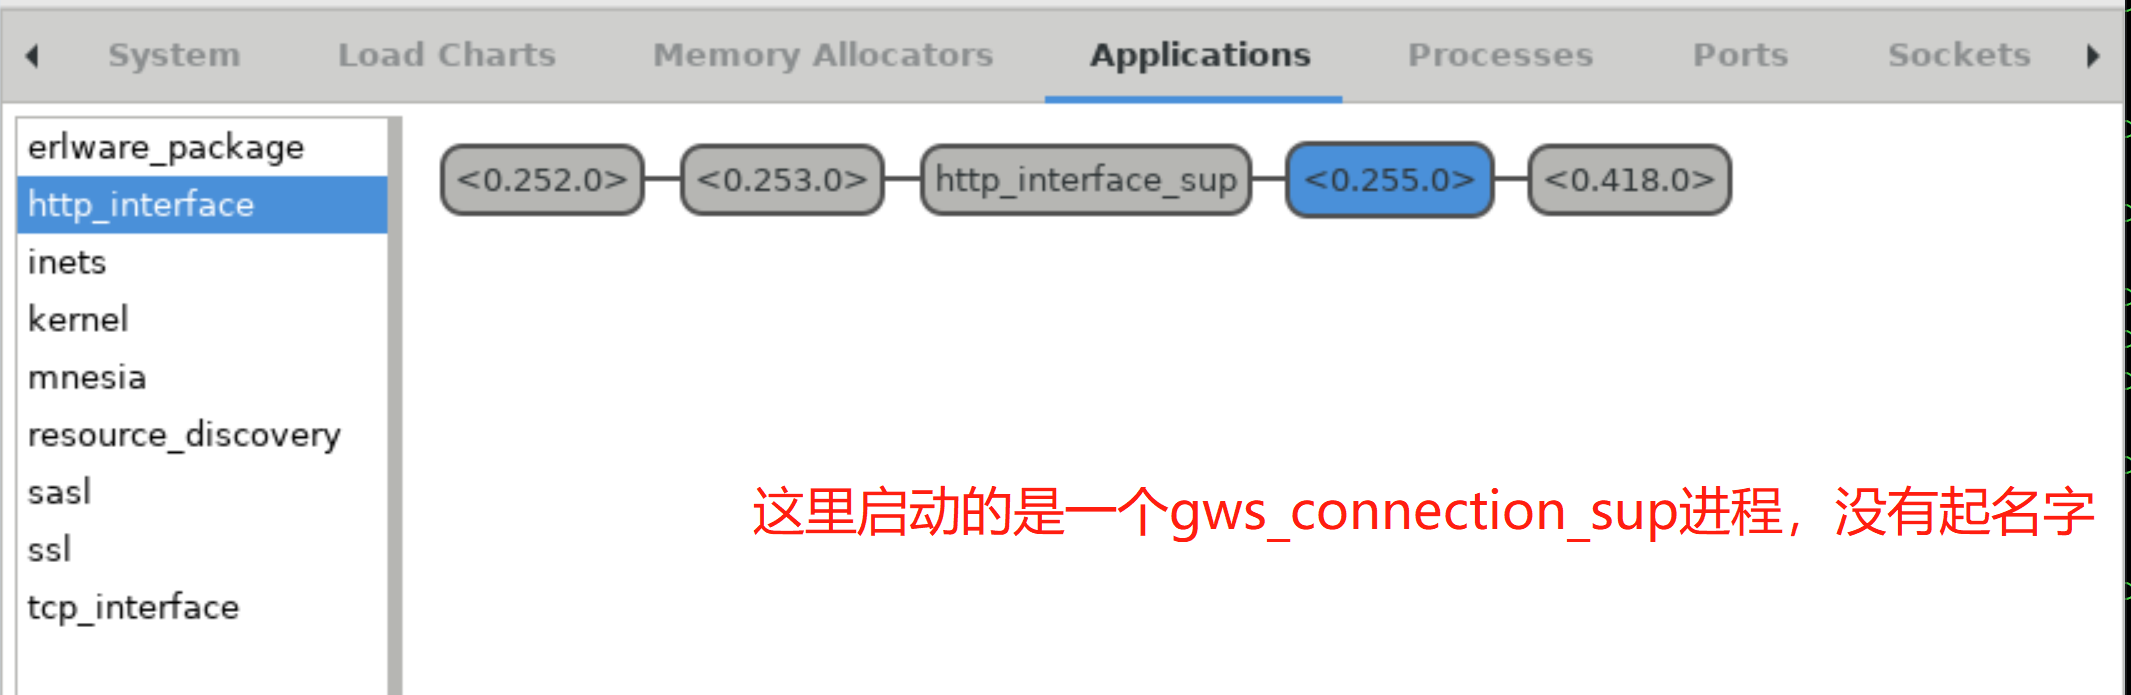
\includegraphics[width=0.85\textwidth]{image58}
\caption{并发编程实践}
\end{figure}

修改了一下，只允许一个实例存在：

\begin{figure}[H]
\centering
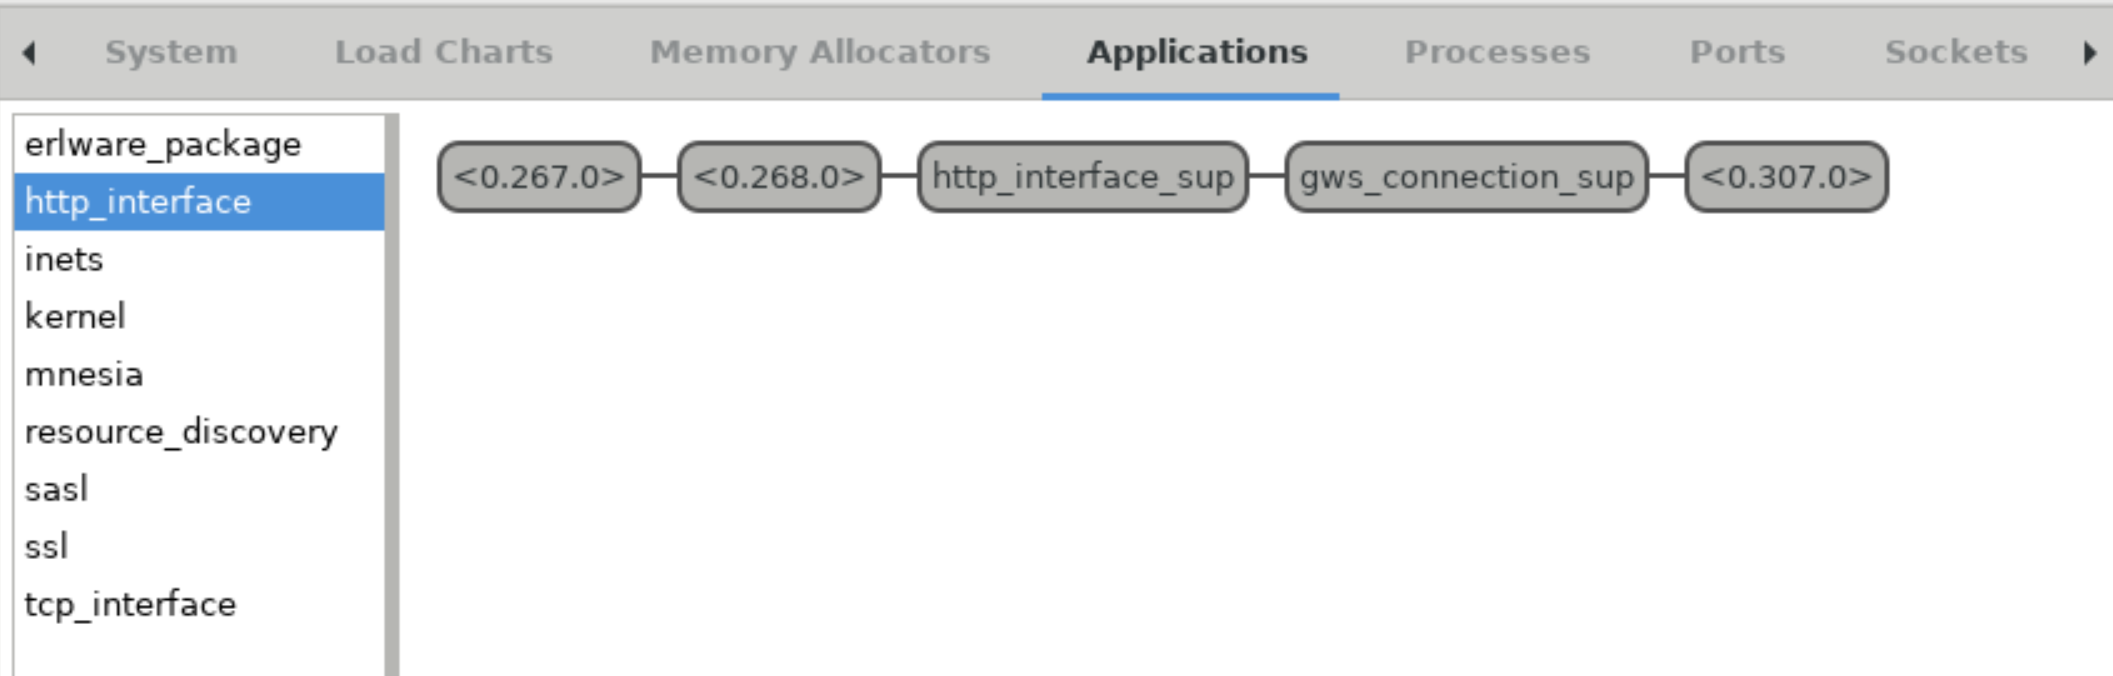
\includegraphics[width=0.85\textwidth]{image59}
\caption{单实例修改}
\end{figure}

% ============================================================
% Section 9: Miscellaneous
% ============================================================
\section{其他知识点}

\subsection{获取系统信息}

\subsection{net\_adm:localhost/0}

\begin{lstlisting}
1> net_adm:localhost().
"centos7-mq1"
\end{lstlisting}

\subsection{监控垃圾回收}

\subsection{清屏}

参考：\href{https://stackoverflow.com/questions/37829916/how-do-i-reset-clear-erlang-terminal}{Stack Overflow - How do I reset/clear erlang terminal}

\subsection{列表打印完全：rp(Term)}

\lstinline|rp(Term)| 使用 shell 已知的 record 定义来打印 term。所有内容都会完整打印，不会像返回值那样限制深度。

\begin{lstlisting}
rp(code:all_loaded()).
\end{lstlisting}

参考：\href{https://www.erlang.org/doc/man/shell.html}{Erlang -- shell}、\href{https://stackoverflow.com/questions/75566211/how-does-it-show-completely-on-erl-terminal-in-erlang}{Stack Overflow}

\subsection{Core Erlang}

\begin{itemize}[leftmargin=1.5em]
    \item \href{https://www.it.uu.se/research/group/hipe/cerl/doc/core_erlang-1.0.3.pdf}{Core Erlang 规范 (PDF)}
    \item \href{https://www.erlang.org/blog/core-erlang-by-example/}{Core Erlang by Example - Erlang/OTP}
    \item \href{https://baha.github.io/intro-core-erlang-2/}{A Gentle Introduction to Core Erlang: Part 2}
    \item \href{https://8thlight.com/insights/the-core-of-erlang}{The Core of Erlang}
\end{itemize}

\end{document}
